\pdftrailerid{}
\pdfinfoomitdate=1
\pdfsuppressptexinfo=-1
\documentclass[11pt]{article}
\usepackage[a4paper,margin=28mm]{geometry}
\usepackage[T1]{fontenc}
\usepackage{mathpazo,microtype}
\renewcommand{\ttdefault}{pcr}
\usepackage{amsmath,amssymb,amsthm,mathtools,bm}
\usepackage{booktabs,longtable,array,graphicx}
\usepackage{tikz}
\usetikzlibrary{arrows.meta,positioning,calc}
\usepackage{xcolor,enumitem}
\usepackage[numbers,sort&compress]{natbib}
\usepackage[colorlinks=true,linkcolor=blue!45!black,citecolor=blue!45!black,urlcolor=blue!45!black]{hyperref}
\usepackage[capitalise,noabbrev,nameinlink]{cleveref}
\usepackage{float}
\usepackage{caption}
\usepackage{listings,upquote}
\lstset{basicstyle=\ttfamily\small,breaklines=true,columns=fullflexible,keepspaces=true}
\setlength{\emergencystretch}{2em}
\setlist{topsep=5pt,itemsep=3pt}
\numberwithin{equation}{section}
\newtheorem{theorem}{Theorem}[section]
\newtheorem{lemma}[theorem]{Lemma}
\newtheorem{proposition}[theorem]{Proposition}
\newtheorem{corollary}[theorem]{Corollary}
\theoremstyle{definition}
\newtheorem{definition}[theorem]{Definition}
\newtheorem{example}[theorem]{Example}
\theoremstyle{remark}
\newtheorem{remark}[theorem]{Remark}
\newcommand{\C}{\mathbb C}
\newcommand{\R}{\mathbb R}
\newcommand{\N}{\mathbb N}
\newcommand{\Z}{\mathbb Z}
\newcommand{\E}{\mathbb E}
\newcommand{\Prob}{\mathbb P}
\DeclareMathOperator{\rank}{rank}
\DeclareMathOperator{\brank}{\underline R}
\DeclareMathOperator{\Vol}{Vol}
\DeclareMathOperator{\supp}{supp}
\DeclareMathOperator{\Tr}{Tr}
\DeclareMathOperator{\diag}{diag}
\DeclareMathOperator{\en}{en}
\newcommand{\HH}{\mathrm H}
\newcommand{\II}{\mathrm I}
\newcommand{\Prb}{\mathbb P}
\newcommand{\colA}{\mathsf A}
\newcommand{\colB}{\mathsf B}
\newcommand{\colC}{\mathsf C}
\newcommand{\ind}{\mathbf 1}
\newcommand{\calF}{\mathcal F}
\newcommand{\calH}{\mathcal H}
\newcommand{\wt}{\operatorname{wt}}
\DeclareMathOperator*{\argmax}{arg\,max}
\title{Complex Matrix Multiplication Below \(2.258\)\\and Rectangular Bounds}
\author{OpenAI}
\date{September 24, 2026}
\hypersetup{pdftitle={Complex Matrix Multiplication Below 2.258 and Rectangular Bounds},pdfauthor={OpenAI},pdfsubject={Arithmetic matrix multiplication exponent and a rigorous finite certificate}}
\begin{document}
\maketitle
\begin{abstract}
Over every field of characteristic zero, we prove that the square
matrix-multiplication exponent satisfies \(\omega<2.258\), the dual exponent
satisfies \(\alpha>0.465\), and \(\omega(1,0.709,1)<2.092\). The strict
square and \(k=0.709\) rectangular bounds also hold over every field except
possibly in one finite set of positive characteristics, in the
arithmetic-operation model.
\end{abstract}
\tableofcontents
\section{Introduction}\label{sec:introduction}

Matrix multiplication asks for the bilinear map \((A,B)\mapsto AB\),
where the two input matrices have compatible sizes.  Its arithmetic
complexity measures the number of field operations needed to compute
all entries of the product.  Except in the field-transfer results
of Section~\ref{sec:characteristic-transfer}, the field is \(\C\), and
the constants in an algorithm may belong to \(\C\).
For \(0\le k\le1\), let
\[
 w(k)=\omega(1,k,1)
\]
be the infimum of exponents for multiplying an
\(n\times\lceil n^k\rceil\) matrix by a
\(\lceil n^k\rceil\times n\) matrix.
The bound \(w(k)\le\tau\) means that for every \(\varepsilon>0\)
these products can be computed using \(O(n^{\tau+\varepsilon})\)
arithmetic operations.
The square exponent is \(\omega=w(1)\), and the dual exponent is
\[
 \alpha=\sup\{k\in[0,1]:w(k)=2\}.
\]
The output size gives \(w(k)\ge2\).  Thus \(\alpha\) measures how far
the inner dimension can grow while multiplication retains the exponent
of its output size.  Square and rectangular multiplication are basic
operations in algebraic algorithms; controlling the rectangular shape
can matter even when a square bound is already available.

\subsection{Context and main result}

Strassen's rank-seven algorithm for \(2\times2\) multiplication gave
\(\omega\le\log_2 7\), establishing subcubic arithmetic complexity
\cite{strassen}.  Approximate bilinear algorithms and their conversion
to exact algorithms \cite{bini}, Sch\"onhage's asymptotic sum inequality
\cite{schonhage}, and Strassen's laser method \cite{strassen-laser}
made tensor powers and degenerations central to subsequent advances.
Coppersmith and Winograd combined low-border-rank tensors with
arithmetic-progression constructions \cite{cw}.  Their extraction
method restricts powers of a small tensor to direct sums of matrix
products, whose dimensions enter the asymptotic sum inequality;
their tensor-square analysis gave \(\omega<2.375477\)
\cite[Section~8]{cw}.
Higher powers and more detailed analyses of these tensors
led to the improvements of Stothers, Vassilevska Williams, and Le Gall
\cite{stothers,williams-powers,legall-powers}.

Rectangular multiplication requires separate control of the three
matrix dimensions.  Early work of Coppersmith and of Lotti and Romani
developed this direction \cite{coppersmith1982,lottiromani1983}; later
constructions of Coppersmith, Le Gall, and Le Gall and Urrutia improved
the available rectangular and dual bounds
\cite{coppersmith-rect,legall-rect,legall-urrutia}.
Recent advances include the refined laser method of Alman and
Vassilevska Williams \cite{alman-williams}, the asymmetric hashing of
Duan, Wu, and Zhou \cite{duan-wu-zhou}, and the square and rectangular
analyses of Vassilevska Williams, Xu, Xu, and Zhou \cite{vxxz} and
Alman, Duan, Vassilevska Williams, Xu, Xu, and Zhou \cite{advxxz}.
The four-author work establishes \(\alpha\ge0.321334\); these two
papers also give detailed tables of rectangular estimates.
Dupont et al.\ subsequently optimized the asymmetric framework at
a larger scale to obtain \(\omega<2.371177\)
\cite{dupont}, a bound incorporated into the updated table of
\cite{advxxz}.

The common extraction problem is to separate many candidate products
that share variables, while accounting for the cost of every operation
used to separate them.  We adjoin auxiliary group tensors that both
resolve shared labels and supply useful matrix-product factors.  Their
full rank cost enters the resulting inequalities.  This construction
gives the following bounds.

\begin{theorem}\label{thm:main}\label{thm:square}\label{thm:rectangular}
Over \(\C\), the arithmetic matrix-multiplication exponents satisfy
\[
 \omega<\frac{1129}{500}=2.258,\qquad
 \alpha>0.465,\qquad w(0.709)<2.092.
\]
\end{theorem}

Corollary~\ref{cor:characteristic-transfer} transfers the strict square
and \(k=0.709\) inequalities to every field of characteristic zero or
outside one finite set of positive characteristics, in the same
arithmetic-operation model.  It selects two fixed exact rank schemes,
realizes their coefficients over one number field, and specializes
their polynomial identities.  The exceptional primes are not computed.
Corollary~\ref{cor:characteristic-zero-dual} also gives the same
dual-exponent bound over every field of characteristic zero.
No dual-exponent transfer in positive characteristic is asserted.

The square bound also lowers the arithmetic exponent of basic
linear-algebra tasks.  Given \(A\in\C^{n\times n}\) and
\(b\in\C^n\), one can compute \(\det A\) and, when \(A\) is
nonsingular, \(A^{-1}\) and the solution of \(Ax=b\), using
\(O(n^c)\) field operations for some fixed \(c<2.258\), with exact
zero tests for pivot selection.  Choose \(\omega<c<2.258\) and apply
the fast elimination reductions of Strassen \cite{strassen} and
Ibarra, Moran, and Hui
\cite[Theorem~2.1 and Corollary~2.1]{ibarra-moran-hui}.

Two applications of the same separation lemma prove the theorem.
The square bound uses finite tensor constructions, a differential
comparison for their attainable values, and an exact numerical
certificate.  The dual and rectangular bounds come from explicit
conditional-label trees and rational entropy certificates.
We also optimize all leaf probability laws in a specified finite
family of such trees, obtaining a bound for every aspect ratio in
\([0,1]\).  The square and rectangular construction families, and
the precise way a square estimate augments the latter, are described
below.

\subsection{Separating labels with an auxiliary tensor}

A trilinear tensor is a sum of monomials \(xyz\), with variables
drawn from three finite coordinate sets \(X,Y,Z\).  Its rank is the
least number of products of three linear forms needed to express it.
A restriction substitutes linear forms separately on the three
sides.  A degeneration allows parameter-dependent substitutions and
takes a leading coefficient.  Border rank is the least rank of
tensors approaching the given tensor.  These operations are local: a
coordinate substitution cannot depend on information visible only
on another side.

Suppose that the supported monomials carry \(K\) labels, and that
each of two sides can independently determine the label from its own
coordinate.  The third side may still share variables between labels.
The pairwise separation lemma, \cref{lem:group}, tensors the input
with a finite abelian group-addition tensor of rank \(K^{1+o(1)}\).
Local projections then give a direct sum over the labels, with a
size-\(K\) dot-product factor on the two original readers in every
summand.  The label is now visible on all three sides.  Dot-product
factors on the three possible reader pairs combine into a matrix
multiplication tensor.

The construction combines Fourier diagonalization of the group tensor
with tags of equal Euclidean norm and a separate constant-inner-product
slice for each tag.  Its geometry adapts Behrend's construction
\cite{behrend}, following the progression-free constructions of Salem
and Spencer \cite{salem-spencer}.  The use of group algebras also has
an established place in the approach of Cohn and Umans
\cite{cohn-umans}; the local separation identity needed here is proved
in full.  It preserves every original coordinate and coefficient,
including additional tensor indices correlated across occurrences.
Consequently the same identity can be applied inside a previously
restricted tensor.  A separate support argument ensures that every
summand counted in an application is nonzero.

Successive separations are organized by exact conditional counts.
Once a preceding label is direct on all three sides, each side can
locate the positions on which the next operation acts.  Fixing the
number of each possible continuation makes the next auxiliary tensor
and the output dimensions common to all branches.  The multinomial
counts and entropy chain rule are the standard method-of-types
tools \cite{shannon1948,csiszar1998}; locality and the uniform tensor
accounting are proved alongside them here.

\subsection{The square bound: finite constructions and comparison}

The square argument starts from the six-term Coppersmith--Winograd
tensor
\[
 T=\sum_{\substack{i+j+k=2\\0\le i,j,k\le2}}x_i y_j z_k,
\]
which has border rank three \cite[Section~7, equation~(10)]{cw}.
A five-term degeneration of \(T\) has three groups, each detectable
on one designated side.  A local degeneration of three copies retains
\(75\) scalar components.  Separating their successive labels gives
the elementary estimate
\(\omega\le9\log3/\log75<2.290108\)
in \cref{thm:elementary}.  This example displays the auxiliary-rank
accounting before the larger construction is introduced.

For a proposed exponent \(\beta\), suppose a finite construction
from \(n\) copies of \(T\) and an auxiliary tensor of border rank
at most \(R\) produces \(L\) independent matrix products of common
dimensions \(a\times b\) by \(b\times c\).  Its normalized score is
\[
 \frac{\log L-\log R+(\beta/3)\log(abc)}{n}.
\]
Sch\"onhage's asymptotic sum inequality implies that a score strictly
greater than \(\log3\) proves \(\omega<\beta\).
Thus the square argument must produce a strict score gain while
retaining the entire auxiliary charge.

We organize the finite constructions by their source distribution.
There are six collections of original tensor occurrences, called
\emph{orientation banks}, one for each permutation of the three
sides.  The distribution records the same exact frequencies in the
original coordinates of each bank.  This keeps a physical permutation
of a tensor distinct from a change of its recorded law.  The square
sections use \(\alpha\) for this vector-valued source law; the dual
exponent in \cref{thm:main} is a scalar.  A construction
preserves arbitrary unresolved tensors attached to its original words,
and its output labels identify distinct surviving words.
Taking the closure of the finite law--score pairs gives a continuous
concave attainable-value function.  Conditional pooling and a new
application of the group separator to each longer pool provide the
composition properties needed in the comparison.

The key analytic step uses restrictions on sums of the local grades
\(i,j,k\).  Each side can read its own sum.  Windows placed at
progression-free target indices force the three locally read targets
to agree, creating another direct label.  The progression-free
construction and the matching argument have the ancestry of Behrend
and Coppersmith--Winograd \cite{behrend,cw}.
To exploit the new labels, a finite-horizon control steers every word
allowed by its controls into the assigned terminal window.  This
every-word guarantee is what permits all the resulting tensor
summands to be counted.  Exact rational prefix populations then
translate the finite control tree into local tensor maps with common
auxiliary supplies.

This construction forces a differential inequality on any smooth
function touching the attainable value from below.  The covariance
of the local grades determines the weighted combination of second
derivatives in this inequality.  Smooth touching
tests and strict comparison follow the viscosity-solution methodology
of Crandall and Lions and of Crandall, Ishii, and Lions
\cite{crandalllions1983,crandallishiilions1992}; the required
inequality and comparison are proved directly from the finite tensor
constructions.  A rational polynomial chart and a polynomial barrier
then give the strict score gain at an interior source distribution.
Boundary constructions supply the initial lower estimates, while
explicit residual, interpolation, and rounding bounds turn the finite
integer checks into inequalities on the entire comparison domain.

Finally, a strict gain in the closed attainable set selects one
actual finite construction with score greater than \(\log3\).
Its law may be close to the chart's central law.  All control horizons,
rational approximations, group sizes, and bank sizes are fixed before
the asymptotic sum inequality is applied.

\subsection{Rectangular bounds and finite-family optimization}

The rectangular argument tracks the three matrix dimensions separately.
A readable label tree partitions a tensor's support until each leaf
is one monomial; at every node, conditional on the preceding labels,
the next child is independently readable on two specified sides.
Fix a rational probability law on its leaves and apply the tree to
an admissible number of copies with those exact leaf frequencies;
arbitrary leaf laws follow by approximation.  The number of child words
at a node is a multinomial coefficient.  The product of these
coefficients is exactly the number of final direct summands, so the
leading auxiliary rank charge is canceled by this multiplicity in
the equal-summand inequality.  The three remaining logarithmic
dimensions are the conditional entropies accumulated on the three
reader pairs.  This is \cref{thm:entropy}.

Explicit polynomial degenerations giving border-rank bounds two and
three supply the initial trees.  Their supports have three colors, with a
designated side able to detect its own color.  A \emph{completion}
takes several copies, chooses a center color, and retains color words
containing at most one distinct noncenter color.  Local color tests
implement this leading-term degeneration and preserve the conditional trees.
Deleting one color at the end gives a fully readable tree.
The family \(\calF_7\) consists of both bases, at most seven
completions of sizes two or three, all center choices, all pairs of
retained colors, and all choices of a distinguished side.

For each member of this finite family, a three-state recurrence
maximizes every nonnegative weighted sum of its incident and
nonincident conditional entropies over all leaf laws.  Its support
function therefore describes the closed downward convex hull of the
normalized rate pairs exactly.  \Cref{thm:shape-optimization} turns
this description into a maximization over one real parameter for
each aspect ratio.  An available square estimate contributes one
additional rate point.  In particular, the square part of
\cref{thm:main} supplies the point for \(p=2.258\).
This finite-family optimization is distinct from the square
attainable-value construction with orientation banks and count windows.

Two explicit laws give the dual and rectangular conclusions.
For the dual exponent, an exact conditional-independence identity
preserves all the entropy of a uniform coordinate word on its incident
reader pairs.  This equality certifies exponent two, and the remaining
entropy certifies the inner dimension.  A small fiber histogram gives
the rectangular point.  Rational enclosures establish their strict
numerical margins.  The same finite family also gives an independent
square bound below \(2.267\) by an integer leaf count.

\Cref{sec:comparison} compares the resulting bounds with the
specified numerical tables of \cite{vxxz,advxxz}, augmented by the
same square point \(p=2.258\) and closed under the ordinary
combination operations stated there.  The new bounds strictly improve
this table baseline for \(0.321334<k<1\).  This comparison concerns
recorded upper estimates.  Extensions to additional estimates retain
their stated separator or envelope hypotheses, and strict improvement
is asserted only where the enlarged baseline itself exceeds two.

\subsection{Organization}

\Cref{sec:preliminaries} establishes the tensor and arithmetic-exponent
conventions.  \Cref{alg:section} proves the shared separation lemma
and the finite tensor constructions.  The square argument begins in
\cref{val:section,ap:section}, which define the attainable values and
prove the count-window comparison.
\Cref{cert:w-seed-section} establishes the three-state boundary
estimate used by the numerical certificate in \cref{cert:section}.
\Cref{sec:conclusion} extracts the finite
witness proving the square part of \cref{thm:main}.
\Cref{sec:trees,sec:completion,sec:optimization} develop conditional
entropy, completion trees, and exact finite-family optimization.
\Cref{sec:certificates} proves the remaining parts of
\cref{thm:main}, and \cref{sec:comparison} gives the baseline
comparisons.  Section~\ref{sec:characteristic-transfer} proves the
finite-exception field corollary from two exact rank witnesses and
the characteristic-zero dual corollary using accuracy-dependent witnesses.
The appendices give barrier coefficients and reproduction details.

\section{Tensors and arithmetic exponents}\label{sec:preliminaries}

We first fix the tensor conventions shared by the square and rectangular
constructions, then relate rank and explicit polynomial degenerations to
arithmetic exponents.  The equal-summand inequality at the end of the
section will convert separated tensors into rectangular bounds.

All vector spaces and tensors are over \(\C\).  A tensor on three finite
coordinate sets \(X,Y,Z\) is identified with a trilinear form
\[
 T=\sum_{x,y,z}T_{xyz}\,x y z.
\]
A restriction is obtained by a linear map on each of the three sides.
In particular, a local zeroing-out sets selected variables on each side
to zero.  A degeneration \(U\unrhd V\) permits these maps to depend
polynomially or Laurent polynomially on a parameter and extracts the
transformed tensor's first nonzero coefficient, after an overall rescaling.
The maps may be composed finitely many times.
Finitely many parameters can be replaced by sufficiently separated powers
of a single parameter.

The rank \(\rank(T)\) is the minimum number of products of three linear
forms whose sum is \(T\).  Its border rank \(\brank(T)\) is the least
integer \(r\) such that tensors of rank at most \(r\) can approach
\(T\).  Border rank is submultiplicative under tensor product and cannot
increase under degeneration.  The direct sum \(U\oplus V\) uses
disjoint variable spaces on all three sides.  A claimed direct sum must
therefore have both disjoint pieces and no additional terms joining their
variables.

Our matrix-multiplication convention is
\[
 \langle a,b,c\rangle
 =\sum_{i=1}^{a}\sum_{j=1}^{b}\sum_{k=1}^{c}x_{ij}y_{jk}z_{ki},
 \qquad \Vol\langle a,b,c\rangle=abc.
\]
For positive integers \(l_1,l_2,l_3\), write
\(\mathcal R(l_1,l_2,l_3)=\rank\langle l_1,l_2,l_3\rangle\).

For \(a_1,a_2,a_3\ge0\), let \(W(a_1,a_2,a_3)\) denote the arithmetic
exponent for the three dimensions \(\lceil n^{a_i}\rceil\).
The trilinear interpretation makes \(W\) invariant under permutations,
including those implemented by transposition.
In particular \(w(k)=W(1,k,1)\).

\begin{lemma}\label{lem:rank-exponent}
For \(a_i\ge0\),
\begin{equation}\label{eq:rank-exponent}
 W(a_1,a_2,a_3)=
 \lim_{s\to\infty}\frac{\log\mathcal R
   (\lceil e^{sa_1}\rceil,\lceil e^{sa_2}\rceil,
          \lceil e^{sa_3}\rceil)}{s}.
\end{equation}
Moreover, \(W\) is coordinatewise nondecreasing, homogeneous,
subadditive, permutation invariant, and continuous.  It satisfies
\[
 W(a_1,a_2,a_3)\ge\max_{i\ne j}(a_i+a_j).
\]
\end{lemma}

\begin{proof}
Fix \(s>0\), put \(l_i=\lceil e^{sa_i}\rceil\), and take a rank-\(r\)
scheme for this triple.  Each of the three flattenings has rank
\(l_i l_j\), so \(r\ge\max_{i\ne j}l_i l_j\).
The scheme applied recursively to blocks of dimensions \(l_i^{h-1}\)
uses \(r\) smaller products and at most a fixed constant times
\((\max_{i\ne j}l_i l_j)^{h-1}\) linear operations at each level.
Its total cost is \(O((h+1)r^h)\).
All products keep a left-input block before a right-input block, so
rectangular block multiplication is legitimate.
Padding with \(h=\lceil t/s\rceil\) proves the corresponding arithmetic
upper bound for arbitrary large dimensions.
The same padding and tensor-power argument shows that the limsup in
\eqref{eq:rank-exponent} is at most the infimum over fixed \(s>0\).
Hence the rank limit exists.

Conversely, a straight-line arithmetic computation of the bilinear
matrix product gives rank at most a constant times its operation count.
Introduce separate formal variables for the two operands and retain
bidegrees at most \((1,1)\).
Each gate introduces only a bounded number of new products of a linear
form in the first operand and one in the second; the remaining mixed
coefficients are linear combinations of earlier ones.
For divisions we use Strassen's division-elimination method
\cite{strassen-division}, in the following bilinear adaptation.
If divisions are allowed, first translate to a generic constant input
at which every denominator is nonzero and use the same truncated-series
argument.  The mixed coefficient of the output is still the desired
bilinear map.
This proves the converse inequality in \eqref{eq:rank-exponent}.

Restriction and padding give monotonicity; tensor products give
subadditivity; rescaling \(s\) gives homogeneity.
These statements include coordinates equal to zero.
For continuity, compare two triples through their coordinatewise
maximum and use the naive bound on the nonnegative increment:
the change in \(W\) is at most the sum of absolute coordinate changes.
Finally the flattening bounds give the displayed lower bound.
\end{proof}

All logarithms in this paper are natural.
The properties in \cref{lem:rank-exponent} imply that \(w\) is convex.
For instance, subadditivity and homogeneity applied to
\(\lambda(1,k_1,1)+(1-\lambda)(1,k_2,1)\) give its usual convexity
inequality.

The approximate bilinear algorithms of \citet{bini} and the
asymptotic-sum method of \citet{schonhage} motivate the following
explicit form of a rank budget.  We use polynomial border-rank witnesses.
Saying that \(T\) has \emph{cost} \(R\) means that \(T\), up to a nonzero
scalar, is the first nonzero coefficient of a polynomial or Laurent
polynomial tensor family with a rank-\(R\) decomposition.
This is a supplied witness and a certified upper bound, which need not
be minimal.  It implies \(\brank(T)\le R\); it is not our definition of
border rank.  All uses of cost below have an explicit witness, so no
converse assertion about arbitrary border-rank limits is needed.
Coordinate restrictions and monomial leading-term degenerations preserve
such witnesses and their budgets.  Finitely many parameters can be
combined into one by assigning sufficiently separated powers, so a
composition of the operations used below again has a univariate witness.

The following interpolation argument is the border-to-exact transfer
for polynomial approximate bilinear algorithms \cite{bini}.

\begin{lemma}\label{lem:border-overhead}
For a fixed tensor of cost \(R\), its \(N\)-th tensor power has exact
rank at most \(O(N+1)R^N\), where the implicit constant may depend on
the fixed witness.
\end{lemma}

\begin{proof}
Clear negative parameter powers.
The degree of the \(N\)-th power of the witness is \(O(N)\), and its
desired coefficient is the \(N\)-th tensor power of the first
coefficient.  Univariate interpolation expresses that coefficient using
\(O(N+1)\) evaluations, each of rank at most \(R^N\).
\end{proof}

A dot tensor on the pair \(Y,Z\) of size \(D\) is
\(x_0\sum_{j=1}^D y_jz_j\).
The product of dot tensors on the three pairs is a matrix-multiplication
tensor.  More precisely, if their lengths on \(XY,XZ,YZ\) are
\(d_{XY},d_{XZ},d_{YZ}\), respectively, their product is
\[
 \langle d_{XZ},d_{XY},d_{YZ}\rangle.
\]
Thus the edge \(XZ\) supplies the index \(i\), the edge \(XY\)
supplies \(j\), and the edge \(YZ\) supplies \(k\) in our convention.
Dot sizes on the same pair multiply.  A tuple of logarithmic edge rates
listed in the order \((XY,XZ,YZ)\) therefore gives matrix-dimension
rates in the order \((XZ,XY,YZ)\).  By the permutation invariance in
Lemma~\ref{lem:rank-exponent}, either order gives the same value of
\(W\).  This accounts for the edge-rate order used in the later
conditional-label entropy bound.

\begin{lemma}[Equal rectangular summands]\label{lem:rectangular-sum}
Suppose a tensor of cost \(R\) restricts or degenerates to a direct sum
of \(M\) copies of the matrix-multiplication tensor with dimensions
\(l_1,l_2,l_3\).  Then
\begin{equation}\label{eq:rectangular-sum}
 W(\log l_1,\log l_2,\log l_3)\le \log R-\log M.
\end{equation}
\end{lemma}

\begin{proof}
Write the left side as \(u\).
If \(u=0\), a flattening of the \(N\)-th power of the direct sum,
together with \cref{lem:border-overhead}, gives
\(M^N\le O(N+1)R^N\); thus \(R\ge M\).

Otherwise choose an integer \(c\) with \(cu>\log M\).
A rank scheme for dimensions \(l_i^{cN}\) can be interpreted as requests
for products of blocks with dimensions \(l_i^N\).
The \(N\)-th power of the direct sum supplies \(M^N\) such requests in
one batch, at cost \(O(N+1)R^N\).
The requests may depend on common inputs: substituting those linear
forms into the independent batch inputs is a restriction.
Pad the last batch if necessary.  Consequently
\[
 \mathcal R(l_1^{(1+c)N},l_2^{(1+c)N},l_3^{(1+c)N})
 \le O(N+1)R^N
 \left\lceil
 \frac{\mathcal R(l_1^{cN},l_2^{cN},l_3^{cN})}{M^N}
 \right\rceil .
\]
By \cref{lem:rank-exponent}, the expression inside the ceiling grows
exponentially because \(cu>\log M\).
Take logarithms, divide by \(N\), and pass to the limit to obtain
\((1+c)u\le \log R+cu-\log M\), proving the claim.
\end{proof}

This is the equal-summand rectangular form of the asymptotic-sum
principle \cite{schonhage}.
The proof applies it to each fixed instance before varying that
instance.  Later auxiliary tensors may therefore grow with a type
parameter without any uniformity assumption on the interpolation
constant in \cref{lem:border-overhead}.

\section{Finite tensor constructions}
\label{alg:section}

The elementary construction in this section already gives
\(\omega\leq 9\log 3/\log 75=2.290107196\ldots\).
Its main ingredient separates a label that two parties can read independently.
The operation supplies the missing label to the third party and leaves a
large dot product.  We pay for the auxiliary tensor that performs this
operation.  At the exponential scale, the new direct labels compensate for
that payment, while the dot product remains available for matrix
multiplication.  We first prove the operation, including its action on
unresolved tensor factors, and then give the finite constructions used later
for the boundary estimates.

\subsection{Pairing conventions and the input rank}
\label{alg:conventions}

We use the tensor and matrix-dimension conventions of
Section~\ref{sec:preliminaries}.
A pairing on \(X,Y\) of length \(m\), with a scalar third side, is
\(\langle1,m,1\rangle\); the other orientations are
\(\langle m,1,1\rangle\) on \(X,Z\) and
\(\langle1,1,m\rangle\) on \(Y,Z\).
Their tensor products satisfy
\begin{equation}
 \langle a,1,1\rangle\otimes\langle1,b,1\rangle
 \otimes\langle1,1,c\rangle\cong\langle a,b,c\rangle.
 \label{alg:pairing-product}
\end{equation}
The logarithmic volumes of such factors therefore add.

The input is the six-term specialization of the Coppersmith--Winograd
tensor \citep[Section~7, equation~(10)]{cw},
\begin{equation}
 T=CW_1=x_2y_0z_0+x_0y_2z_0+x_0y_0z_2
        +x_0y_1z_1+x_1y_0z_1+x_1y_1z_0.
 \label{alg:cw}
\end{equation}
Write
\(\mathcal S=\{200,020,002,011,101,110\}\) for its support, abbreviating
\((i,j,k)\) by \(ijk\).  At every position the three indices sum to two.
The maps in our square construction for this input have algebraic
coefficients.  The general preservation identities below also allow
arbitrary complex coefficients in the unresolved tensors.

\begin{lemma}
\label{alg:cw-rank}
The tensor \(T\) has border rank three.  Consequently
\(\brank(T^{\otimes n})\leq3^n\) for every integer \(n\geq1\).
\end{lemma}
\begin{proof}
Let \(\zeta=e^{2\pi i/3}\), and put
\[
 X_r(t)=x_0+\zeta^r t x_1+\zeta^{2r}t^2x_2
 \quad (r=0,1,2),
\]
with analogous definitions for \(Y_r,Z_r\).  Filtering the degree modulo
three gives the exact identity
\[
 \frac{1}{3t^2}\sum_{r=0}^2\zeta^r X_r(t)Y_r(t)Z_r(t)
 =T+t^3(x_2y_2z_1+x_2y_1z_2+x_1y_2z_2).
\]
For every nonzero \(t\), the left side has rank at most three.  Taking
\(t\to0\) proves the upper bound.  In the flattening with the \(X\) side
as rows, the three coefficients of \(x_0,x_1,x_2\) are linearly independent:
the monomials \(y_0z_2,y_0z_1,y_0z_0\), respectively, distinguish them.
The flattening rank is therefore three, giving the reverse bound.  Tensoring
the upper-bound construction proves the last assertion.
The displayed identity also supplies an explicit polynomial witness of
cost three in the terminology of Section~\ref{sec:preliminaries}.
\end{proof}

We use the following established theorem in exactly its border-rank form;
see also the explicit statement in
\citet[Theorem~3.1]{afl}.

\begin{theorem}[Asymptotic sum inequality, \citet{schonhage}]
\label{thm:asi}
If a tensor \(U\) degenerates to
\(\bigoplus_{\ell=1}^{L}\langle a_\ell,b_\ell,c_\ell\rangle\), with all
dimensions positive integers, then
\[
 \sum_{\ell=1}^{L}(a_\ell b_\ell c_\ell)^{\omega/3}
 \leq\brank(U).
\]
In particular, if
\(T^{\otimes n}\otimes\mathcal A\unrhd
\bigoplus_{\ell=1}^{L}\langle a,b,c\rangle\)
and \(\brank(\mathcal A)\leq R\), then
\begin{equation}
 L(abc)^{\omega/3}\leq3^nR.
 \label{alg:asi-account}
\end{equation}
\end{theorem}

The auxiliary rank \(R\) in \eqref{alg:asi-account} is part of the input
cost.  Thus, for a proposed exponent \(\beta\), a finite realization with
\begin{equation}
 \log L-\log R+\frac{\beta}{3}\log(abc)>n\log3
 \label{alg:strict-score}
\end{equation}
proves \(\omega<\beta\).  We never cancel an auxiliary tensor as a tensor
identity; only its explicitly charged logarithmic rank will be offset by
output multiplicity.

\subsection{Supplying a label to its missing party}
\label{alg:group-section}
\label{sec:separation}

Suppose a tensor is partitioned into pieces whose \(X\)-variables are
disjoint and whose \(Y\)-variables are disjoint.  Each of these two parties
can then determine the same piece label from its own variable.  The
\(Z\)-variables may still be shared.  The next lemma resolves this last
sharing without resolving the terms inside a piece.  We call this operation
GROUP.

The construction uses equal-norm shells, following the geometry of
\citet{behrend}, together with affine slices that constrain two independently
chosen auxiliary indices.  Its auxiliary tensor is the multiplication
tensor of a finite abelian group, linking the construction to the
group-theoretic tensor approach of \citet{cohn-umans}.  The identity and its
full rank charge are proved below.

\begin{lemma}[Pairwise label separation]
\label{lem:group}
\label{lem:separator}
Let \(U=\sum_{s=1}^{K}U_s\), where \(U_s\) uses \(X\)-variables in
\(X_s\) and \(Y\)-variables in \(Y_s\), and the families
\((X_s)_{s=1}^K\) and \((Y_s)_{s=1}^K\) are each disjoint.  The
\(Z\)-variables may overlap.  There are a finite abelian group \(G\), its
group multiplication tensor \(\mathcal A_G\), and a positive integer
\(m\) such that
\begin{equation}
 U\otimes\mathcal A_G\unrhd
 \bigoplus_{s=1}^{K}\bigl(U_s\otimes\langle1,m,1\rangle\bigr).
 \label{alg:group-identity}
\end{equation}
The degeneration is a zeroing-out on auxiliary coordinates controlled by
the original local variables.  It preserves all original coordinates and
coefficients.  For \(K\to\infty\), the parameters can be chosen with
\begin{equation}
 \rank(\mathcal A_G)=\brank(\mathcal A_G)=|G|,
 \qquad
 \log|G|=\log K+O(\sqrt{\log K}),
 \qquad
 m=K.
 \label{alg:group-rates}
\end{equation}
The same statement holds for any other pair of knowing sides.
\end{lemma}
\begin{proof}
The case \(K=1\) uses the trivial group and \(m=1\), so no
nontrivial auxiliary tensor is needed.
For \(K\geq2\), set
\[
 d=\lceil\sqrt{\log K}\rceil+3,
 \qquad
 Q=\left\lceil((d+1)K)^{1/(d-2)}\right\rceil,
 \qquad m=K.
\]
Since \(dQ^2+1\leq(d+1)Q^2\), these choices give
\(Q^d/(dQ^2+1)\geq K\).
The grid \(\{0,\ldots,Q-1\}^d\) has \(Q^d\) points and at most
\(d(Q-1)^2+1\) possible squared norms.  Pigeonholing supplies at least
\(K\) distinct points \(t_1,\ldots,t_K\) on one Euclidean sphere.
Assign \(t_s\) to label \(s\).

For each \(s\), the integer inner product \(t_s\cdot u\), as \(u\)
ranges over this grid, has at most \(d(Q-1)^2+1\) values.  A further
pigeonhole argument supplies a set \(V_s\) of at least \(m\) grid points
on one affine slice
\[
 t_s\cdot u=h_s.
\]
Trim each \(V_s\) to exactly \(m\) points.  Only the common inner product
within a slice is needed; the points of a slice need not have equal norm.

Take
\[
 G=(\Z/(4Q)\Z)^d,
 \qquad
 \mathcal A_G=\sum_{a+b=c}\mathsf{x}_a\mathsf{y}_b\mathsf{z}_c,
\]
using separate auxiliary variables on the three sides.  For completeness,
character orthogonality gives a rank decomposition
\[
 \mathcal A_G=\frac1{|G|}\sum_{\chi\in\widehat G}
 \left(\sum_{a\in G}\chi(a)\mathsf{x}_a\right)
 \left(\sum_{b\in G}\chi(b)\mathsf{y}_b\right)
 \left(\sum_{c\in G}\chi(-c)\mathsf{z}_c\right).
\]
It has \(|G|\) summands.  The \(X\)-flattening has \(|G|\) linearly
independent rows, since the coefficient of
\(\mathsf{y}_0\mathsf{z}_a\) distinguishes row
\(a\).  This proves both rank equalities.

For an original \(X\)-variable in \(X_s\), retain auxiliary coordinates
\(a=u\in V_s\).  For an original \(Y\)-variable in \(Y_s\), retain
\(b=t_s-u'\) with \(u'\in V_s\).  On the \(Z\) side retain only
\(c\in\{t_1,\ldots,t_K\}\).  Negative coordinates of \(t_s-u'\)
are interpreted modulo \(4Q\).  These are three local variable
projections: each knowing side uses the label determined by its original
variable, and the third side uses only the prescribed tag set.

A surviving term satisfies
\(c\equiv t_s+u-u'\pmod{4Q}\).
Each coordinate of \(c-t_s-u+u'\) has absolute value at most
\(2(Q-1)<4Q\), so the congruence is an equality of integer vectors.
The tag norms are equal and
\(t_s\cdot(u-u')=0\), whence
\[
 0=\|c\|^2-\|t_s\|^2=\|u-u'\|^2.
\]
Thus \(u=u'\) and \(c=t_s\).  Conversely, every \(u\in V_s\) gives
one surviving triple \((u,t_s-u,t_s)\).
The auxiliary factor in piece \(s\) is precisely
\[
 \sum_{u\in V_s}\mathsf{x}_u\mathsf{y}_{t_s-u}\mathsf{z}_{t_s},
\]
a length-\(m\) pairing on the knowing sides.  The pieces were already
disjoint on those sides and now have distinct auxiliary tags on the third.
The calculation also excludes every cross term, proving
\eqref{alg:group-identity}.

Finally, with \(L=\log K\), the displayed choice of \(d,Q\) satisfies
\[
 d\log Q
 \leq\frac{d}{d-2}\bigl(L+\log(d+1)\bigr)+o(1)
 =L+O(\sqrt L).
\]
The rounding error in \(\log Q\) is exponentially small in
\(\sqrt L\).  Since \(K\leq Q^d\) and
\(|G|=(4Q)^d\), these inequalities and \(m=K\) prove
\eqref{alg:group-rates}.
\end{proof}

For repeated uses at different label counts, fix one such group \(G_K\)
for each \(K\), and write \(A_K=\mathcal A_{G_K}\).  This is the
auxiliary-tensor notation used in the conditional-label entropy bound.

The geometry rules out a stronger collision than the usual
three-term-progression condition: the two slice points \(u,u'\) are chosen
independently.  Their difference is perpendicular to \(t_s\); any nonzero
such displacement from \(t_s\) lies outside its sphere.  Requiring the
endpoint to be another tag therefore forces that difference to vanish.
Figure~\ref{fig:group-geometry} shows this displacement argument.

\begin{figure}[H]
\centering
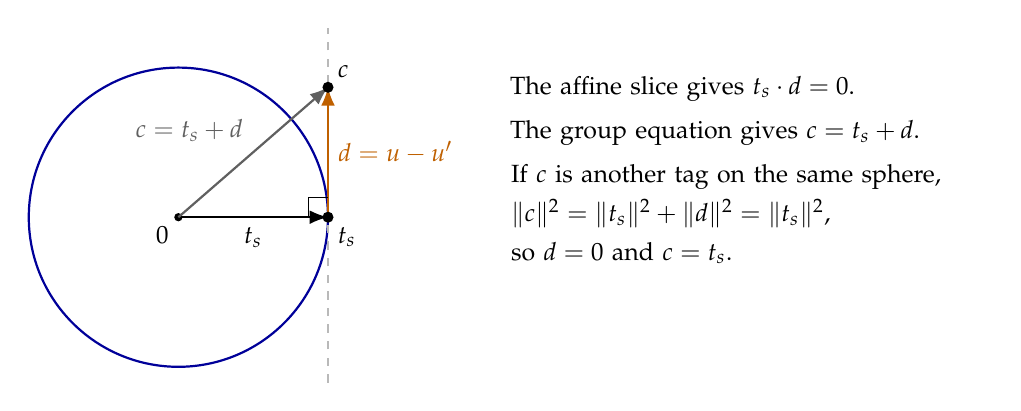
\begin{tikzpicture}[>=Latex,scale=1.0,font=\small]
\draw[blue!60!black,thick] (0,0) circle (1.9);
\draw[gray!55,dashed] (1.9,-2.1)--(1.9,2.4);
\fill (0,0) circle(1.5pt) node[below left] {\(0\)};
\coordinate (tag) at (1.9,0);
\coordinate (candidate) at (1.9,1.65);
\draw[->,thick] (0,0)--(tag) node[midway,below] {\(t_s\)};
\draw[->,thick,orange!75!black] (tag)--(candidate) node[midway,right] {\(d=u-u'\)};
\draw[->,thick,gray!75!black] (0,0)--(candidate) node[midway,above left] {\(c=t_s+d\)};
\fill (tag) circle(2pt) node[below right] {\(t_s\)};
\fill (candidate) circle(2pt) node[above right] {\(c\)};
\draw (1.65,0)--(1.65,.25)--(1.9,.25);
\node[align=left,anchor=west,text width=6cm] at (4.1,0.6) {
The affine slice gives \(t_s\cdot d=0\).\\[5pt]
The group equation gives \(c=t_s+d\).\\[5pt]
If \(c\) is another tag on the same sphere,\\[3pt]
\(\|c\|^2=\|t_s\|^2+\|d\|^2=\|t_s\|^2\),\\[3pt]
so \(d=0\) and \(c=t_s\).
};
\end{tikzpicture}
\caption{The separation identity in a two-dimensional slice.
The dashed line represents the displacement hyperplane
\(t_s+t_s^\perp\), rather than the slice containing \(u,u'\).
A nonzero displacement along it leaves the tag sphere, so no other tag
can survive. The argument applies in every dimension.}
\label{fig:group-geometry}
\end{figure}


\begin{lemma}[Preservation of unresolved fibers]
\label{alg:payload}
The identity in Lemma~\ref{lem:group} holds with arbitrary coefficients
and arbitrary unresolved local indices inside the tensors \(U_s\),
including indices correlated between different original occurrences.
Local support projections and monomial leading-term restrictions have the
same property.  Finite compositions of these operations may leave all
previously produced matrix multiplication factors untouched.
\end{lemma}
\begin{proof}
Retain an original basis coordinate on every side throughout the
construction.  In Lemma~\ref{lem:group}, a surviving auxiliary triple is
characterized solely by the piece label and the equation just proved.
The original coefficient is neither changed nor combined with another
coefficient.  Appending additional local indices to any original variable
therefore gives the same identity for every coefficient separately.  The
extra indices may be arbitrary; no product distribution or independence
between occurrences is used.

A local support projection has the same coefficientwise description.
For a monomial restriction, the degree of each term is the sum of three
local degrees, and its leading coefficient is either its original
coefficient or zero.  This too commutes with adjoining unresolved
coordinates or earlier local count predicates.  The claim for a finite
composition follows by induction.  At each subsequent stage, tensor the
new maps with the identity on all previously produced pairings.
\end{proof}

This preservation statement is a locality statement, not a nonvanishing
statement.  If an earlier support restriction makes a designated source
word absent, its fiber is zero and cannot be counted as an output.  Our
finite constructions below explicitly retain every counted word.  The
later count construction will require a separate guarantee for every
complete controlled path.

\subsection{Exact types and a finite hierarchy of labels}
\label{alg:hierarchy-section}

For a probability vector \(p\) on a finite alphabet, write
\(H(p)=-\sum_i p_i\log p_i\), with \(0\log0=0\).
Exact types provide the finite counting form of entropy used here;
see \citet{csiszar1998} for the method of types.
For rational \(p\) and admissible integers \(N\), the number of words
having exactly \(Np_i\) occurrences of symbol \(i\) is
\begin{equation}
 \binom{N}{(Np_i)_i}
 =\exp\bigl(NH(p)+O(\log(N+1))\bigr).
 \label{alg:type-count}
\end{equation}
The implicit constant depends only on the fixed alphabet.  We use exact
types so that the number of positions assigned to every later conditional
operation is independent of the previously selected direct output.

The following lemma makes precise how multiple separation steps share
auxiliary tensors and count each label once.  Its accounting is the
conditional-entropy chain rule \citep{shannon1948}, applied to labels
that the tensor maps can actually read.

\begin{lemma}[Accounting for a finite label hierarchy]
\label{lem:hierarchy}
Let \(b\geq1\), and let \(\mathcal B\subseteq\mathcal S^b\) be
nonempty.  Suppose local restrictions and degenerations of
\(T^{\otimes b}\) retain exactly these original scalar components, with
their original coordinates and coefficients.  Suppose there are finitely many
labels \(S_1,\ldots,S_t\), each a function of a component in
\(\mathcal B\), with these properties:
\begin{enumerate}[label=\textup{(\roman*)}]
 \item the complete record \((S_1,\ldots,S_t)\) determines the original
       component;
 \item after the earlier labels are fixed, the next label is independently
       readable by two fixed sides within that conditional pool;
 \item every component designated by a retained complete record survives
       all the local restrictions.
\end{enumerate}
Let \(\alpha\) be a rational probability distribution on \(\mathcal B\).
For admissible \(N\to\infty\), there are auxiliary tensors
\(\mathcal A_N\) and degenerations of
\(T^{\otimes bN}\otimes\mathcal A_N\) into \(L_N\) independent matrix
multiplication tensors of common volume \(v_N\), with
\(\brank(\mathcal A_N)\leq R_N\), such that
\begin{equation}
 \log L_N=NH(\alpha)+o(N),\qquad
 \log R_N=NH(\alpha)+o(N),\qquad
 \log v_N=NH(\alpha)+o(N).
 \label{alg:hierarchy-rates}
\end{equation}
When \(H(\alpha)>0\), this gives
\(\omega\leq3b\log3/H(\alpha)\).
\end{lemma}
\begin{proof}
Apply the stipulated local restrictions in each of the \(N\) blocks.
At layer \(j\), write \(h=(S_1,\ldots,S_{j-1})\) for a preceding
record, let \(p_h\) be its probability under \(\alpha\), and let
\(p_{s\mid h}\) be the conditional law of \(S_j\).
The earlier layers have made the full preceding-label word direct on all
three sides.  In every branch there are exactly \(Np_h\) block positions
in conditional pool \(h\).  Each knowing side can read the next-label
word in those positions.  It can therefore zero variables whose next-label
word does not have counts \(Np_hp_{s\mid h}\).  This is a genuine local
type projection, not a presumed projection onto an unavailable joint type.

There remain
\[
 K_{j,h}=\binom{Np_h}{(Np_hp_{s\mid h})_s}
\]
possible next-label words in this pool.  Use Lemma~\ref{lem:group} to
separate them.  A zero-probability pool is omitted, and a deterministic
next label needs no auxiliary tensor.  For a positive-entropy pool,
\eqref{alg:type-count} and \eqref{alg:group-rates} give identical leading
logarithmic contributions
\[
 Np_h H(S_j\mid h)+o(N)
\]
to its direct count, auxiliary rank, and pairing volume.

The auxiliary tensor for pool \((j,h)\) is appended once.  It is reused
in every preceding direct branch through a block-diagonal map: on a direct
sum, each of the three parties knows the branch, so it may address the
appropriate positions using that branch's label.  Equivalently,
\((\bigoplus_\ell V_\ell)\otimes\mathcal A\) is the direct sum of the
\(V_\ell\otimes\mathcal A\), and separate maps may act in its blocks.
This does not charge \(\rank(\mathcal A)\) once per \(\ell\).
The size and physical orientation of every conditional supply depend only
on \((j,h)\), whose population is fixed, not on the selected output word.

There are only finitely many layers and conditional pools.  Multiplying
their counts, ranks, and pairing volumes, and using the entropy chain rule,
gives in each case the leading logarithm
\[
 N\sum_{j=1}^t H(S_j\mid S_1,\ldots,S_{j-1})=NH(\alpha).
\]
All error terms sum to \(o(N)\).  The complete record determines one
original scalar component in each block, and every such designated
component is nonzero by assumption.  Exact conditional counts fix the
number of pairings in each physical orientation.  Formula
\eqref{alg:pairing-product} therefore gives a common matrix multiplication
tensor in all final branches.  This proves \eqref{alg:hierarchy-rates}.
Substituting them in \eqref{alg:asi-account}, dividing by \(N\), and taking
the limit proves the exponent bound.
\end{proof}

Nothing in this lemma permits arbitrary support deletion.  The locally
obtainable support and the two-sided readability must be established for
each hierarchy.  Once they are established, exact conditional types select
its desired joint frequencies through accessible labels.

\subsection{An explicit four-component construction}
\label{alg:four}

First remove the term \(101\) from \(T\).  Scale each of
\(x_1,z_1,y_0,y_2\) by \(t\).  The five other terms have degree one in
\(t\), whereas \(101\) has degree three.  Dividing by \(t\) and taking
the limit gives
\begin{equation}
 T\unrhd T'=A+B+C,
 \quad
 A=x_0(y_0z_2+y_1z_1),\quad
 B=(x_2y_0+x_1y_1)z_0,\quad
 C=x_0y_2z_0.
 \label{alg:five}
\end{equation}
A local predicate on each side identifies exactly one group:
\(Z>0\) identifies \(A\), \(X>0\) identifies \(B\), and \(Y=2\)
identifies \(C\).  Exactly one of these predicates holds on every retained
term.  We call any such three-group partition a \emph{W-partition}; the
three predicates, rather than the original numerical indices, are its
one-hot flags.

Delete \(C\) by setting \(y_2=0\), and take \((A+B)^{\otimes N}\),
with \(4\mid N\).  Retain coarse words with \(N/2\) copies of \(A\)
and \(N/2\) copies of \(B\).  This is local on \(X\), since a zero
\(X\) index means \(A\) and a positive one means \(B\).
The \(Z\) side also identifies the word, with the roles reversed.
There are \(\binom{N}{N/2}\) coarse words.  Lemma~\ref{lem:group}
separates them by supplying their label to \(Y\), and gives each word a
pairing on \(X,Z\) of logarithmic length \(N\log2+o(N)\).

Inside a fixed coarse word, \(A\)'s two terms \(002,011\) are each
identified by \(Y\) and by \(Z\).  Retain \(N/4\) occurrences of each
among the \(N/2\) \(A\) positions and separate their words.  This adds a
pairing on \(Y,Z\) of logarithmic length \((N/2)\log2+o(N)\).
Similarly, \(B\)'s two terms \(200,110\) are each identified by
\(X,Y\); resolving their equal-frequency words adds a pairing on
\(X,Y\) of the same logarithmic length.  These restrictions are
conditional on the already-direct coarse word and therefore are local.

The three pairings combine by \eqref{alg:pairing-product}.  The total
logarithmic output count, auxiliary rank, and volume are each
\(N\log4+o(N)\).  Theorem~\ref{thm:asi} consequently gives
\begin{equation}
 \omega\leq\frac{3\log3}{\log4}=2.377443751\ldots.
 \label{alg:four-bound}
\end{equation}
The scalar original terms alone would not supply any volume to which
\(\omega\) could be applied.  Here the three pairing orientations supply
that volume, while all three auxiliary rank costs have been included.

\subsection{Completion and the 75-component bound}
\label{alg:completion-section}

A W-partition has a useful local description even when its three groups
contain unresolved tensors: side \(i\) knows precisely the positions at
which its own group occurs.  This permits a degeneration of a block of
several occurrences before any group has been made direct.  We call the
following operation COMPLETE.

\begin{lemma}[Completion]
\label{alg:completion}
Let a tensor have a W-partition with labels \(0,1,2\).  For an integer
\(b\geq1\), a local monomial degeneration of its \(b\)-th power retains
exactly the coarse words
\begin{equation}
 \{0,1\}^b\ \cup\ \{0,2\}^b.
 \label{alg:complete-support}
\end{equation}
This support has a new W-partition: the constant word \(0^b\), the words
containing \(1\), and the words containing \(2\).  Conditional on either
nonzero new label, the original binary word is independently readable by
two sides.  The construction preserves arbitrary unresolved fibers.
\end{lemma}
\begin{proof}
The three local predicates are
\[
 \text{every position has label }0,\qquad
 \text{some position has label }1,\qquad
 \text{some position has label }2.
\]
Each is readable on the correspondingly active side of the original
W-partition.  Their sum is one on \eqref{alg:complete-support} and two
when both \(1\) and \(2\) occur.  Multiply a variable by \(t\) when its
predicate holds, divide the tensor by \(t\), and take the limit.  The
surviving predicates form a new one-hot partition.  In the nonzero group
\(i\in\{1,2\}\), the word uses only \(0,i\), so either of those two
active sides determines the entire word from the positions of its own
label.  The degeneration is coefficientwise and hence preserves the fibers
by Lemma~\ref{alg:payload}.
\end{proof}

For the groups \(A,B,C\) in \eqref{alg:five}, assign labels \(0,1,2\)
in that order.  The group sizes are \(2,2,1\).  A completed block has
three group sizes
\[
 2^b,\qquad4^b-2^b,\qquad3^b-2^b.
\]
Delete its all-\(A\) group: its active \(Z\) predicate is that every
original index is positive.  The remaining groups will be denoted
\(P_B\) and \(P_C\).  The \(X\) side recognizes \(P_B\) by the
occurrence of a positive index, and the \(Y\) side recognizes \(P_C\)
by the occurrence of index two.  Since only these two groups remain,
either side independently determines which group occurs.

\begin{theorem}[Elementary completion bound]
\label{thm:elementary}
For every integer \(b\geq2\),
\begin{equation}
 \omega\leq
 \frac{3b\log3}{\log(4^b+3^b-2^{b+1})}.
 \label{alg:complete-bound}
\end{equation}
In particular,
\[
 \omega\leq\frac{9\log3}{\log75}=2.290107196\ldots.
\]
\end{theorem}
\begin{proof}
Apply \eqref{alg:five} to each occurrence, perform the completion of
Lemma~\ref{alg:completion} in blocks of size \(b\), and delete the
all-\(A\) group as just described.  This locally retains
\(s_b=4^b+3^b-2^{b+1}\) original scalar components per block.
Here is a complete hierarchy that separates them.

First resolve the binary group label \(P_B,P_C\), known on \(X,Y\).
After it is direct, resolve the original word inside each group: the
\(A,B\) word in \(P_B\) is known on \(Z,X\), and the \(A,C\) word
in \(P_C\) is known on \(Z,Y\).  After that word is direct, resolve
\(002\) versus \(011\) in every \(A\) position using \(Y,Z\), and
\(200\) versus \(110\) in every \(B\) position using \(X,Y\).
There is no internal choice in \(C\).  The complete record identifies
one original scalar component.  Every such component survives the stated
monomial restriction and deletion.  The pair of knowing sides at each
stage is fixed by the preceding direct labels.

Give the \(s_b\) components equal frequency and apply
Lemma~\ref{lem:hierarchy}.  Their entropy is \(\log s_b\), while the
original rank cost per block is at most \(3^b\).  This proves
\eqref{alg:complete-bound}.

For \(b=3\), the sizes of \(P_B,P_C\) are \(56,19\).  The prescribed
outer frequencies are \(56/75,19/75\); the internal component law in
each group is uniform.  The entropy identity
\[
 H(56/75,19/75)+\frac{56}{75}\log56+\frac{19}{75}\log19=\log75
\]
shows explicitly how the successive choices count each of the 75 terms
once.  Over \(N\) such blocks the three leading logarithms are
\(\log L_N=\log R_N=\log v_N=N\log75+o(N)\).
Using the input cost \(3^{3N}R_N\) in
\eqref{alg:asi-account} and canceling the \emph{logarithmic} multiplicity
and auxiliary costs leaves
\((\omega/3)\log75\leq3\log3\), as claimed.
\end{proof}

The neighboring block lengths illustrate that this particular completion
is not monotone in \(b\):
\begin{center}
\begin{tabular}{@{}ccc@{}}
\toprule
Block length & Retained scalar components & Exponent bound \\
\midrule
2 & 17 & \(2.326571610\ldots\) \\
3 & 75 & \(2.290107196\ldots\) \\
4 & 305 & \(2.304655406\ldots\) \\
\bottomrule
\end{tabular}
\end{center}
No optimization claim over all restrictions of the corresponding power is
needed.  The length-three construction already gives the stated bound.

\subsection{Parity and conditional W constructions}
\label{alg:parity-section}

Completion gives one way of making a new W-partition.  A different local
restriction on three occurrences supplies two useful W labels, which can
be resolved in either order.  We call this operation PARITY.

\begin{lemma}[Parity restriction]
\label{alg:parity}
In three W-partitioned occurrences, a local monomial degeneration removes
exactly the six words in which all three labels occur and retains the
other 21 coarse words.  On the retained support, the majority label and
the odd-count label each define a W-partition.  Once both labels are direct,
the remaining choice is either deterministic or independently readable by
two sides.  All statements remain true with arbitrary unresolved fibers.
\end{lemma}
\begin{proof}
Let \(n_i\) be the count of label \(i\) among the three positions.
Side \(i\) knows its occurrence set and hence \(n_i\).
Scale a variable by \(t^{n_i\bmod2}\) on that side.
The sum of the three parity exponents is one for count patterns
\((3,0,0)\) and \((2,1,0)\), up to permutation, and three for
\((1,1,1)\).  Division by \(t\) and passage to the limit gives the
claimed support.

On this support exactly one label has count at least two, and exactly one
has odd count.  Both are local unary tests, giving the two W-partitions.
Write these labels as \(c,h\).  If \(c=h\), the word is \(ccc\).
Otherwise, it consists of two \(c\)'s and one \(h\).  The \(c\) side
knows the two majority positions and the \(h\) side knows the singleton
position.  Either determines which of the three placements occurs, so
Lemma~\ref{lem:group} applies after \(c,h\) have been made direct.
All restrictions and the final separation preserve fibers by
Lemma~\ref{alg:payload}.
\end{proof}

If the three occurrences have internal scalar counts
\((a_i)_i,(b_i)_i,(c_i)_i\), the fiber with majority \(i\) and odd-count
label \(j\) has size
\begin{equation}
 M_{ij}=
 \begin{cases}
  a_ib_ic_i,&i=j,\\
  a_ib_ic_j+a_ib_jc_i+a_jb_ic_i,&i\ne j.
 \end{cases}
 \label{alg:parity-weights}
\end{equation}
Each term for \(i\ne j\) describes one singleton placement.
For the boundary weights \((2,2,1)\) on all three occurrences, this is
\[
 (M_{ij})=\begin{pmatrix}8&24&12\\24&8&12\\6&6&1\end{pmatrix}.
\]
For example, delete the third majority row and resolve the remaining
binary majority label.  Within the first direct row delete its first
odd-count column; within the second direct row delete its second column.
These are permitted conditional local deletions because the majority is
already direct.  Each row then has size 36, giving 72 original scalar
components.  Lemma~\ref{lem:hierarchy} yields
\(\omega\leq9\log3/\log72=2.311966920\ldots\).
This illustrative restriction is weaker than Theorem~\ref{thm:elementary}.
Parity is useful because its two conditional groupings enlarge the finite
construction family at nonuniform distributions.

\subsection{Finite recipes and weighted laws}
\label{alg:recipes}

We now track the source law and score of a finite tree of W constructions.
Fix labels \(0,1,2\) on each original W-partitioned occurrence before
applying the tree.  These are its \emph{canonical labels}: later physical
permutations may change which side reads a flag, but the original labels
are still counted in this fixed ordering.

For the score calculations below, fix a finite operation tree and its
rational conditional laws.  Admissible exact-type populations, together
with the efficient GROUP tensors of \eqref{alg:group-rates}, give a family
of finite realizations.  The \emph{limiting score} of this fixed tree and
law data is the limit along increasing populations; each member remains
one finite recipe with fixed tensor supplies and maps.
A later operation may depend on a label only once that label is direct on
all three sides.  At every stage, previously produced pairings are separate
tensor factors; their internal indices are never used to choose subsequent
controls.

For a realization on \(n\) original occurrences, let \(L\) be its direct
multiplicity, \(R\) its auxiliary rank bound, and \(v\) its additional
matrix multiplication volume.  The rates are
\[
 D=\frac{\log L}{n},\qquad A=\frac{\log R}{n},\qquad
 M=\frac{\log v}{n}.
\]
Here \(M\) excludes any tensor initially present inside a coarse group.
For the W recipes the convenient formal score is
\(u_\gamma=\gamma(D-A)+M\), where \(\gamma\geq1\).
For \(0<\beta\leq3\),
\[
 u_{3/\beta}=\frac3\beta\left(D-A+\frac\beta3M\right).
\]
Thus \(u_\gamma\) rescales the normalized score expression in
\eqref{alg:strict-score} so that the coefficient of the added volume is one.
Its definition assumes no bound on \(\omega\).
Definitions~\ref{def:strong} and~\ref{val:def-value} will specify the
banked realizations and the closure of their law--score pairs.
For a fixed tree consisting only of
pairwise separation, completion, parity, and conditional exact types,
its total \(D-A\) tends to zero when the group/type supplies grow.
Consequently its limiting score is independent of \(\gamma\).

A binary leaf deletes one W label locally and resolves the remaining
binary word by Lemma~\ref{lem:group}.  At law \(q\) on that pair, its
limiting score is \(H(q)\).  If positive numbers \(d_i\) are assigned as
weights for choosing a law, the weighted score is
\(H(q)+\sum_iq_i\log d_i\).  Maximizing on the retained pair \(i,j\)
gives \(\log(d_i+d_j)\).  These weights may guide selection of a finite
rational law; they do not change the coefficients of a tensor.

For completion of \(b\) occurrences with weights \(d_{r,i}\), the three
fiber weights are
\begin{equation}
 w_0=\prod_{r=1}^b d_{r,0},\qquad
 w_i=\prod_{r=1}^b(d_{r,0}+d_{r,i})-\prod_{r=1}^b d_{r,0}
 \quad(i=1,2).
 \label{alg:complete-weights}
\end{equation}
When the weights are scalar term counts, this is literal counting of the
supports in Lemma~\ref{alg:completion}.  For arbitrary positive weights
it is the corresponding generating polynomial.  For parity the analogous
matrix is \eqref{alg:parity-weights}.

\subsection{Physical orientations and canonical laws}

A physical permutation acts on the full tensor factors of an occurrence or
completed block.  Each original occurrence keeps both its canonical label
and its net physical side permutation.  For
\(\sigma\in\mathfrak S_3\), the \emph{orientation bank} \(\sigma\)
is the collection of original occurrences with that net permutation
relative to their canonical coordinates.  We will arrange that all six
banks have the same exact canonical label histogram.  Their common
normalized histogram is the source law; it is not the aggregate law of the
physical flags after the bank orientations are forgotten.

The exact types used below fix canonical histograms within each relative
orientation.  The next lemma shows how the six global physical permutations
then distribute these counts equally among the original banks, while
keeping one common auxiliary supply.

\begin{lemma}[Equal physical orientation supplies]
\label{alg:orientation-banks}
Fix a finite oriented schedule of operations with prescribed exact
conditional populations.  Suppose its exact types fix, for each relative
physical permutation \(\tau\in\mathfrak S_3\), the canonical input
histogram \(H_\tau\) of all original occurrences with that permutation,
independently of the direct history.  Include all six global physical side
permutations of this schedule, with the same prescribed populations and
histograms in corresponding replicas.
Then every original orientation bank has the same exact canonical input
histogram.  Auxiliary supplies and pairing dimensions are independent of
the direct history.  All regroupings controlled by preceding direct labels
are implementable by local block-diagonal maps.
\end{lemma}
\begin{proof}
In the replica with global permutation \(\sigma\), an original occurrence
of relative orientation \(\tau\) has absolute orientation
\(\sigma\tau\).  Thus an absolute bank \(\rho\) receives the histogram
\(H_\tau\) from the unique replica
\(\sigma=\rho\tau^{-1}\).  Its total histogram is
\[
 \sum_{\tau\in\mathfrak S_3}H_\tau,
\]
independently of \(\rho\) and of the direct history.  The occurrence
positions contributing to a histogram may vary with the history, but its
counts are fixed by hypothesis.  Each original occurrence is counted once,
in its relative-orientation class.

All parties know a preceding direct label, so each can reorder or address
the same specified positions using its own local coordinate map.
Corresponding relative permutations address corresponding physical banks;
no party is required to read another party's local flag.  Each fixed pool
uses a fixed auxiliary tensor and fixed pairing lengths.  Tensoring all
those supplies once and acting block-diagonally therefore gives uniform
rank bounds and dimensions.  Previously produced pairings remain untouched.
\end{proof}

In particular, rotating the flags of an intermediate completed block
changes its grouping and its readers, but does not recode the labels of
the original occurrences inside it.  To recover a canonical label from a
physically permuted occurrence, undo that occurrence's permutation.

\subsection{Resolving and composing nested recipes}

An operation in the finite library may complete two occurrences, physically
transpose that completed block, and then complete it with a third
occurrence.  Resolving its original word calls for a hierarchy inside the
final fiber.  The following statement supplies that hierarchy for any
fixed finite composition of completion gates.

\begin{lemma}[Resolving a tree of completion gates]
\label{alg:completion-hierarchy}
Consider a finite rooted tree whose leaves are W-partitioned occurrences
and whose internal nodes apply Lemma~\ref{alg:completion} to their children.
Before a child is used at a parent, allow a fixed physical permutation of
that whole child block.  The retained support has a W-partition at its
root.  Once the root label is direct, the original leaf-label word admits
a finite hierarchy of pairwise-readable refinements.  All refinements
preserve arbitrary unresolved leaf fibers.

In a fixed root fiber, let \(P\) be any rational law on the retained
original leaf-label words.  Across \(N\) copies of that fiber, exact
conditional types and Lemma~\ref{lem:group} give direct multiplicity,
auxiliary rank bound, and added pairing volume whose logarithms are each
\(NH(P)+o(N)\).  The auxiliary product and pairing dimensions are common
to every direct output.  Canonical original labels are unchanged by the
intermediate physical permutations.
\end{lemma}
\begin{proof}
Process the nodes from the root toward the leaves.  Suppose a node's label
is already direct, and express its children's W labels in that node's
current physical coordinates.  If the node label is zero, completion
forces all those child labels to be zero.  Otherwise, if its label is
\(i\in\{1,2\}\), its child-label word lies in \(\{0,i\}^b\), where
\(b\) is the number of children.  Side zero knows the positions with label
zero and side \(i\) knows the positions with label \(i\); either side
determines the word.  Apply Lemma~\ref{lem:group} to separate that word.
Every child label is now direct on all three sides.  Undo the known
physical permutation on its label to identify the child's own root label,
and recurse into that child.  Recursion is required even when the parent
label was zero: a known child root may still contain unresolved choices.

There are finitely many nodes.  Each successive refinement is a function
of the original leaf word, and the complete record recovers that word.
For the law \(P\), prescribe the induced rational conditional type of
each refinement in each preceding direct pool.  These types are locally
readable by the two sides just identified.  They fix all pool populations,
so a single prescribed auxiliary product can be used by block-diagonal
maps in every branch.  They also fix the counts of pairings in every
physical orientation.  As in the proof of Lemma~\ref{lem:hierarchy}, each
pool contributes its conditional entropy to all three leading logarithms.
The chain rule sums these contributions to \(H(P)\), since the complete
record and the original leaf word determine one another.  The output
pairing dimensions are therefore common to all branches.

The retained support is exactly the intersection of the primitive
completion conditions, each implemented by its local monomial
degeneration.  Every word in \(P\)'s support satisfies those conditions.
Lemma~\ref{alg:payload} preserves any unresolved leaf fibers through every
step.  A physical permutation changes the sides reading a node's flags;
the final histogram still counts each leaf in its original canonical
coordinates.  To apply Lemma~\ref{alg:orientation-banks}, let \(\tau_r\)
be the relative physical permutation of original leaf \(r\).  The exact
full-word law \(P\) fixes the count of canonical label \(i\) in relative
orientation \(\tau\) to be
\[
 H_{\tau,i}
 =N\sum_w P(w)\,
       \#\{r:\tau_r=\tau,\ w_r=i\}.
\]
These counts are independent of the direct output.  The lemma therefore
supplies equal original orientation banks when this schedule is taken in
all six global orientations.  No individual occurrence is required to carry
a fixed letter.
\end{proof}

To spell out the three-position case used in the library, let \(c(i,j)\)
be the two-child completion label: it is zero for \((i,j)=(0,0)\), and
is \(a\in\{1,2\}\) if both entries belong to \(\{0,a\}\) and at
least one equals \(a\).  It is undefined on \((1,2),(2,1)\).  Write
\[
 a=c(i,j),\qquad z=a-k\pmod3,\qquad s=c(z,r),
 \quad k\in\{0,1,2\}.
\]
The subtraction by \(k\) represents the physical rotation of the whole
first completed block.  In a fixed final fiber \(s\), first resolve the
top-level operand labels \((z,r)\).  This fixes \(a=z+k\pmod3\),
after which the inner word \((i,j)\) can be resolved using the pair of
sides belonging to that inner completion, with its physical rotation
included.  If \(C_s\) is an arbitrary rational law on the retained
triples, the two levels supply
\begin{equation}
 H(C_s)=H(Z,R\mid S=s)
       +\sum_{z,r}\Prob(Z=z,R=r\mid S=s)
                      H(I,J\mid Z=z,R=r,S=s).
 \label{alg:nested-completion-entropy}
\end{equation}
Here \(Z\) is a deterministic function of \(I,J\), so no intermediate
label adds a second entropy count.  The intermediate rotation changes
the grouping flag and its physical reader; it does not recode \(I,J,R\)
when the original canonical word histogram is calculated.

\begin{proposition}[Composition of finite recipe laws]
\label{alg:recipe-composition}
Consider a primitive completion, a finite tree of completion gates as in
Lemma~\ref{alg:completion-hierarchy}, or a parity operation on \(b\)
original occurrences.
Let \(s\) be its outer W label, with a rational law \(a_s\), separated
by a fixed recipe tree with limiting score \(u_0\).  In the outer group \(s\),
let \(t\) be a further W label, with conditional rational law \(r_{st}\),
separated by a fixed recipe tree with limiting score \(u_s\).
For completion this label is deterministic and \(u_s=0\).
For parity it is the other of the majority and odd-count labels.
For each permitted \((s,t)\), choose a rational distribution \(P_{st}\)
on its remaining original coarse words.  If \(n_i(w)\) counts canonical
input label \(i\) in the word \(w\), then the resulting original law and
limiting score are
\begin{align}
 q_i&=\frac1b\sum_{s,t}a_s r_{st}\,
                   \mathbb E_{w\sim P_{st}}n_i(w),
       \label{alg:recipe-law}\\
 u&=\frac1b\left(u_0+\sum_s a_su_s
                     +\sum_{s,t}a_s r_{st}H(P_{st})\right).
       \label{alg:recipe-score}
\end{align}
The formula is feasible for every stipulated finite collection of child
recipes and rational distributions; no optimality assertion is required.
\end{proposition}
\begin{proof}
Use the outer child recipe while the internal choices remain unresolved
fibers.  Its coordinate-preserving identity is valid by
Lemma~\ref{alg:payload}.  Once its label is direct, apply the corresponding
conditional child in each group.  The group populations are fixed by exact
types, so the prescribed auxiliary product is appended once and shared by
all branches.  After these labels are direct, resolve the remaining words
by the hierarchy in Lemma~\ref{alg:completion-hierarchy} for completion,
or by the single remaining pairwise-readable placement in
Lemma~\ref{alg:parity}.  Prescribe the conditional types induced by
\(P_{st}\) at every refinement.  Their conditional entropies sum to
\(H(P_{st})\), and Lemma~\ref{lem:group} supplies exactly this limiting
score across the hierarchy.  The relative population of that pool is
\(a_sr_{st}\).

The same types provide the histograms required for banking.  The outer and
conditional child recipes fix the number of macro occurrences assigned to
each \((s,t)\) pool in each of their original banks.  Within every such
pool, impose the full-word law \(P_{st}\) through its readable refinements.
For each original leaf position, this law fixes its marginal counts across
the pool, just as in the preceding proof.  Grouping those contributions by
the leaf's relative physical permutation fixes the total histograms
\(H_\tau\).  This uses each child's whole-bank histogram and the new
full-word types, not a fixed letter at an individual position of a child
recipe.  Lemma~\ref{alg:orientation-banks} now makes the final canonical
law common to all six original banks.

Logarithms of counts, auxiliary rank bounds, and pairing volumes add.
Dividing their sum by the number \(b\) of original occurrences per new
block proves \eqref{alg:recipe-score}.  Counting the original labels in
the same conditional pools proves \eqref{alg:recipe-law}.  A finite common
multiple of the rational denominators and the fixed child bank sizes
makes all pool sizes integral.  Increasing these supplies makes the finitely
many group and type errors vanish.  Every counted original coarse word
survives the stipulated support restrictions, so the outputs on the scalar
W input are nonzero.  Arbitrary unresolved fibers are preserved
coefficientwise; a zero attached fiber remains zero.
\end{proof}

The words in \eqref{alg:recipe-law} are counted in their original canonical
coordinates.  The resulting \(q\) is the exact common law of the original
orientation banks, providing the finite input to the banked-value
construction of the next section.

\section{Banked constructions and attainable values}
\label{val:section}

A local separation identity must remain valid when the positions on which it
acts are correlated with positions to be processed later.  It is also necessary
to distinguish a distribution in the coordinates of a tensor from the
aggregate distribution after physically permuting its sides.  We make both
requirements explicit.  This gives the finite objects whose attainable values
will enter the differential comparison.

\subsection{Canonical banks and preservation of unresolved tensors}
\label{val:banks}

Let $\mathcal S=\{200,020,002,011,101,110\}$ and
$\mathcal W=\{100,010,001\}$.  The latter is the support of the ordinary
three-state tensor
\[
 \mathsf W=x_1y_0z_0+x_0y_1z_0+x_0y_0z_1.
\]
An element of either alphabet is a triple of local grades.
We use $\mathcal B$ to denote either alphabet in definitions
that apply to both.  Write $\mathfrak S_3$ for the group of permutations of the
three tensor sides.  A \emph{banked input of size $N$} has $N$ occurrences in
each orientation $\sigma\in\mathfrak S_3$, for a total of $n=6N$
occurrences.  Its original component words are
\[
 w=(w_{\sigma,t})_{\sigma\in\mathfrak S_3,\ 1\le t\le N},
 \qquad w_{\sigma,t}\in\mathcal B.
\]
The triple $w_{\sigma,t}$ is expressed in canonical coordinates: its physical
grade triple is $\sigma w_{\sigma,t}$.  Thus physical side $j$ observes the
canonical coordinate $\sigma^{-1}(j)$.  Both $T$ and the ordinary $\mathsf W$ tensor
are symmetric under these physical permutations, so this banking does not
change the underlying input tensor.  Its purpose is to record types and
permitted transposes accurately.

A banked word has exact law $\alpha\in\Delta(\mathcal B)$ if, separately for
each $\sigma$, every symbol $s$ occurs $N\alpha_s$ times.  In particular,
$\alpha$ is not the histogram obtained by forgetting the bank orientations.
All normalizations below divide by $6N$.

We allow additional, unresolved local indices.  To state the preservation
requirement precisely, for every original component word $w$ attach an
arbitrary three-tensor $P_w$ on these additional indices.  The tensors $P_w$
may share their variable spaces, may correlate all the positions, and may be
zero.  Denote the resulting input by $\mathcal T(P)$: its restriction to the
original word $w$ is the original scalar component at $w$ tensored with
$P_w$.  This description includes preceding local count restrictions by
setting the corresponding fibers to zero.  It does not assert that all such
families arise as independent products.

\begin{definition}[Strong banked realization]
\label{def:strong}
A strong realization consists of a finite auxiliary tensor $\mathcal A$, a
finite degeneration by three local maps, a set $\Lambda$ of direct labels,
and positive integers $a,b,c$, with the following properties.
\begin{enumerate}[label=\textup{(\roman*)}]
\item Every $\lambda\in\Lambda$ designates an original word $w(\lambda)$,
      and $\lambda\mapsto w(\lambda)$ is injective.  All these words have
      the same exact canonical law in each orientation bank.
\item For every family of unresolved tensors $P=(P_w)$ the same maps give
\begin{equation}
\mathcal T(P)\otimes\mathcal A
 \unrhd
 \bigoplus_{\lambda\in\Lambda}
 \bigl(P_{w(\lambda)}\otimes\langle a,b,c\rangle\bigr).
\label{val:strong-identity}
\end{equation}
      In this display the original local coordinates of $w(\lambda)$ are
      retained as well; only their fixed basis factors are suppressed.
      Original coefficients and unresolved local indices are unchanged.
\item The auxiliary input, its charged border-rank bound, and the output
      dimensions $a,b,c$ are independent of $\lambda$.
\end{enumerate}
The identity is required also for zero $P_w$.  Such an output is a formal
zero fiber and contributes no nonzero direct summand.  A realization used in
an attainable-value calculation must separately establish that all its
counted fibers are nonzero on its specified input.
\end{definition}

The maps in this paper retain each original local index and act on auxiliary
coordinates conditionally on that index and on already direct labels.
Consequently they commute with local projections depending only on the
original indices.  The same statement holds when the maps are expressed as
leading monomial degenerations.  This observation concerns locality; it does
not prove nonvanishing after an earlier projection.  Nonvanishing will be
checked by support identities for the algebraic primitives and by the
universal path condition in Lemma~\ref{lem:compile} for arithmetic-progression
(AP) count constructions.

Lemma~\ref{lem:group} supplies \eqref{val:strong-identity} term by term.
Indeed its sphere and slice argument decides the retained auxiliary terms
without referring to any coefficient of $P_w$.  Local singleton projections
and direct matchings have the same preservation property.  The conditional
composition rules of Section~\ref{val:recipes} use only these identities;
they never presume independence of unresolved fibers.

For the banking operation of Lemma~\ref{alg:orientation-banks}, group the
original input occurrences of a finite schedule by their relative physical
orientation $\tau$.  The lemma requires their total canonical histogram
$H_\tau$ to be fixed independently of the direct history and shared by all
six globally permuted replicas.  Exact types of complete original words
supply these grouped histograms in the completion and parity recipes.
When an already strong child is physically permuted as a whole, each of
its original input banks supplies a fixed histogram by
Definition~\ref{def:strong}.  The letter at an individual position may
still vary between direct outputs.

In outer replica $\sigma$, the group of relative orientation $\tau$ has
absolute orientation $\sigma\tau$.  Each absolute bank therefore receives
one copy of $H_\tau$ for every $\tau$, and has histogram
$\sum_\tau H_\tau$.  Equal conditional pool sizes alone would not imply
this histogram identity.  The pool sizes instead fix how many child calls
and auxiliary supplies are used; the grouped types or strong child banks
supply the required letter counts.  A physical permutation of an
intermediate macro acts on every original occurrence inside it.

\subsection{Finite recipes and the closure of their values}
\label{val:recipes}

A \emph{structural recipe} is a finite expression describing local
projections and leading degenerations, direct-label-controlled maps, locally
imposed exact joint and conditional types, auxiliary GROUP calls, and tensor
products on specified collections of positions.  Its bank sizes, rational types, and
integer group parameters are finite.  A conditional choice is permitted only
after its controlling label is direct on all three sides.  Each byproduct
matrix multiplication factor is kept as a separate factor: later decisions
use original-word labels and do not read, identify, or spend its indices.

We use the following two classes of such recipes.
\begin{enumerate}[label=\textup{(\alph*)}]
\item The $\mathsf W$ class starts with singleton projections, binary deletion
      followed by GROUP, and the finite COMPLETE and PARITY compositions
      of Proposition~\ref{alg:recipe-composition}.  It allows rational
      time-sharing on separate positions, physical permutation banking,
      and finite AP count compositions of previously constructed recipes.
\item The six-state class starts with singleton projections, the direct
      matching construction of Proposition~\ref{prop:matching}, and the
      five-state face substitutions of Proposition~\ref{prop:face} using
      finite $\mathsf W$ recipes.  It has the same time-sharing, banking, and finite
      AP closure.
\end{enumerate}
Both classes also allow two explicit finite rearrangements.  First, one
may reindex the orientation banks by $\sigma\mapsto\sigma\tau$ for a fixed
$\tau\in\mathfrak S_3$, with the corresponding canonical letter relabeling;
Lemma~\ref{val:canonical-symmetry} proves its precise effect.  Second, one
may \emph{conditionally recompile} an earlier finite recipe: expand its
finite direct-label refinement tree, take finitely many replicas, impose a
rational exact type of complete terminal transcripts through its induced
conditional types, and replace corresponding GROUP calls by GROUP on the
longer conditional pools.  All other original support predicates are retained
on their old macroblocks.  This is a finite construction rule using the same
local primitives, not an operation on scores.  Its instances must preserve
Definition~\ref{def:strong} and nonzero support like every other recipe;
Lemma~\ref{val:recompile} proves those requirements for the uniform terminal
type used below.  Neither rearrangement authorizes an infinite composition.

Here an AP composition is the finite count-window construction of
Lemma~\ref{lem:compile}.  Its children are finite recipes, not calls to an
attainable-value function.  The full expression can therefore be expanded to
a finite tree.  Equivalently, take the union of all finite levels of this
construction rule.  The $\mathsf W$ class is defined independently of the six-state
class.

A recipe belongs to these classes only when its local identities establish
Definition~\ref{def:strong}, its counted original words survive all of its
restrictions, and its auxiliary profile and output dimensions are fixed
across its direct histories.  These are algebraic conditions, not inequalities
for numerical scores.  The primitive support proofs, exact conditional-type
composition, and Lemma~\ref{lem:compile} establish these conditions for the
listed generators.  In particular, introducing the AP closure here does not
assume the differential inequality that it will later prove.

The auxiliary tensor in every recipe is a product of finite group tensors.
We charge the product of their ranks, which is also their tensor product's
rank by Fourier diagonalization and flattening.  It is harmless to charge a
larger certified bound.  No tensor already present in an unresolved fiber is
included in the byproduct volume.

For a realization with $n=6N$ original occurrences, $L=|\Lambda|$ counted
nonzero direct summands, auxiliary rank bound $R$, and common additional
volume $v=abc$, put
\begin{equation}
 D=\frac{\log L}{n},\qquad
 A=\frac{\log R}{n},\qquad
 M=\frac{\log v}{n}.
\label{val:rates}
\end{equation}
For $0<\beta\le3$ and $\gamma\ge1$, respectively, the two scores are
\begin{equation}
 f_\beta=D-A+\frac\beta3M,
 \qquad
 u_\gamma=\gamma(D-A)+M.
\label{val:scores}
\end{equation}
These are formal tensor rates.  Their definitions impose no assumption on
$\omega$.  In particular, on the same realization
$u_{3/\beta}=(3/\beta)f_\beta$.

\begin{definition}[Attainable-value functions]
\label{val:def-value}
For each finite realization let $\alpha$ be its canonical bank law.  Take all
pairs $(\alpha,t)$ with $t$ no greater than its score, and take their ordinary
Euclidean closure in $\Delta(\mathcal B)\times\R$.  The upper boundaries of
these closed sets are denoted by $F_\beta(\alpha)$ for the six-state class
and $U^W_\gamma(q)$ for the $\mathsf W$ class.
\end{definition}

Allowing smaller scores makes these sets downward closed.  The closure allows
irrational laws and limits of finite recipes of increasing size; it does not
introduce an infinite composition acting on a finite tensor.  In particular,
if $F_\beta(\alpha)>c$, then some actual finite realization has score greater
than $c$, possibly at a law arbitrarily close to $\alpha$.

\begin{proposition}[Bounds, concavity, and continuity]
\label{prop:values}
For $0<\beta\le3$ and $\gamma\ge1$,
\begin{equation}
 0\le F_\beta(\alpha)\le H(\alpha)\le\log6,
 \qquad
 0\le U^W_\gamma(q)\le\gamma H(q)\le\gamma\log3.
\label{val:entropy-cap}
\end{equation}
Both functions are concave and continuous on their closed probability
simplices.  They have supporting affine functionals at every relative
interior point.
\end{proposition}

\begin{proof}
Every additional pairing has size at most the rank charged for its group
tensor.  Because byproducts remain separate, their volumes multiply, and
$M\le A$.  Source-word injectivity and exact types give
\[
 L\le\left(\frac{N!}{\prod_s(N\alpha_s)!}\right)^6
 \le \exp(6NH(\alpha)),
 \qquad D\le H(\alpha).
\]
The same formula holds with the $\mathsf W$ alphabet.  Thus $f_\beta\le D$ and
$u_\gamma\le\gamma D$, proving the upper bounds also after closure.

A specified original word can be retained by singleton projections.  Taking
one such word of any prescribed rational type in each bank gives $L=R=v=1$
and score zero.  Density supplies the lower bound zero at every law.

To mix two finite constructions, repeat them enough times that a rational
fraction $\lambda$ of the positions in each orientation is allocated to the
first and the remaining fraction to the second.  Tensor their maps, auxiliary
inputs, and outputs.  The new law and score are
\[
 \lambda\alpha^{(1)}+(1-\lambda)\alpha^{(2)},\qquad
 \lambda f^{(1)}+(1-\lambda)f^{(2)}.
\]
Their direct transcripts inject into concatenated original words, all bank
histograms and dimensions remain uniform, and all support conditions are
preserved.  Rational approximation and closure give concavity for real
$\lambda$ and limiting laws.

For upper semicontinuity, suppose $\alpha_k\to\alpha$.  The upper bounds in
\eqref{val:entropy-cap} give a bounded subsequence of values approaching the
limsup.  Approximate each value by a pair in the defining closed set.  Closedness
then places the limiting pair in that set, so its value is at most the value
at $\alpha$.  This also shows that each finite upper boundary is attained in
the closed set.

For lower semicontinuity at any $\alpha$, including at a face, set
\[
 \varepsilon_k=
 \max_{s:\alpha_s>0}
       \left(1-\frac{\alpha_{k,s}}{\alpha_s}\right)_+.
\]
Then $\varepsilon_k\to0$.  If $\varepsilon_k>0$, the vector
\[
 r_k=\frac{\alpha_k-(1-\varepsilon_k)\alpha}{\varepsilon_k}
\]
is a probability vector.  Indeed its coordinates are nonnegative, including
those where $\alpha_s=0$, and its total is one.  Concavity and nonnegativity
give $F_\beta(\alpha_k)\ge(1-\varepsilon_k)F_\beta(\alpha)$.
If $\varepsilon_k=0$, conservation of total mass implies
$\alpha_k=\alpha$.  This proves lower semicontinuity; the proof for $U^W_\gamma$
is identical.  A finite continuous concave function has a supporting affine
functional at each relative interior point, by separation of its hypograph.
\end{proof}

\begin{lemma}[Symmetry of canonical laws]
\label{val:canonical-symmetry}
For $\tau\in\mathfrak S_3$, define
$(\tau_*\alpha)(s)=\alpha(\tau^{-1}s)$.  Then
\[
 F_\beta(\tau_*\alpha)=F_\beta(\alpha),\qquad
 U^W_\gamma(\tau_*q)=U^W_\gamma(q).
\]
\end{lemma}

\begin{proof}
Start with a strong realization and move old bank $\sigma\tau$ to new bank
$\sigma$, reinterpreting its canonical symbol $s$ as $\tau s$.  The physical
grade is unchanged, because $\sigma(\tau s)=(\sigma\tau)s$.  This is a
fixed permutation of original occurrence positions, performed identically
on all three sides, together with a change of canonical bookkeeping.
Conjugate the old local maps by this position permutation.  Their
coordinatewise identities continue to hold for arbitrary unresolved tensors,
with the same relabeling of their original positions.  Every new bank has
canonical law $\tau_*\alpha$.  Source-word injectivity, nonzero support,
the auxiliary tensor, and all byproduct dimensions are unchanged.  Thus the
same $D,A,M$ are attained at the permuted law.  The inverse rearrangement
uses $\tau^{-1}$; taking closures proves both equalities.  This canonical
law symmetry is distinct from replicating a schedule in all six physical
orientations, which preserves its canonical law.
\end{proof}

\begin{remark}[A useful exact-law correction]
\label{val:dilution}
If a construction or a convex mixture has law $\widehat\alpha$, and a desired
law $\alpha$ has positive coordinates, put
\[
 \lambda=\max_{s:\widehat\alpha_s>0}
 \left(1-\frac{\alpha_s}{\widehat\alpha_s}\right)_+.
\]
For $\lambda>0$, the vector
$r=(\alpha-(1-\lambda)\widehat\alpha)/\lambda$ is a probability law.
Mixing the construction with singleton constructions of average law $r$
therefore gives $\alpha$ exactly, at loss at most $K\lambda$ if the old score
is at most $K$, where $K\ge0$.  Moreover
\[
 \lambda\le
 \max_s\frac{(\widehat\alpha_s-\alpha_s)_+}{\alpha_s}.
\]
When the data are rational, this is a finite rational time-sharing operation.
For limiting data it is justified by the defining closure.  This correction
will be used when converting approximate finite laws to exact target laws.
\end{remark}

\subsection{Conditional pooling and monotonicity in the formal parameter}
\label{val:pooling}

A finite GROUP call pays a small excess of auxiliary rank over its number of
labels.  Tensor-repeating that particular finite map does not remove its
normalized excess.  The following lemma replaces each GROUP call by a new
one acting on a long conditional pool.  It is the requisite justification for
monotonicity in $\gamma$.  The face substitution below evaluates the W value
at $\gamma=3/\beta$; monotonicity will let the certificate use a lower
estimate obtained at a smaller formal parameter.

\begin{lemma}[Recompiling a fixed finite recipe]
\label{val:recompile}
Fix a finite recipe on $n$ original occurrences with canonical law $q$, $L$
terminal labels, charged auxiliary rank $R$, and additional volume $v$.
Fix $\gamma\ge1$.  There is a sequence of recipes on larger exact banks,
with the same canonical law $q$, such that
\begin{equation}
 \liminf u_\gamma^{\mathrm{new}}
 \ge \frac{\gamma\log L-\gamma\log R+\log v}{n},
 \qquad
 \liminf(D^{\mathrm{new}}-A^{\mathrm{new}})\ge0.
\label{val:recompile-goal}
\end{equation}
All source-word restrictions of the old recipe hold separately in every old
macroblock of the new recipes.
\end{lemma}

\begin{proof}
Expand the fixed recipe into its finite sequence of conditional refinements,
including the finite recipes used at any earlier AP nodes.  Refine a history
whenever its next local operation, its informed pair, or its auxiliary
parameters differ.  Terminal histories can be padded by deterministic steps
so that every transcript is a leaf of one finite decision tree.  Every
intermediate label is determined by the designated original word: GROUP
labels encode its source label sequence, matching labels identify the word,
coarse flags are functions of it, and AP labels are fixed by its disjoint
count windows.  Thus this expansion adds no terminal multiplicity; its leaves
are exactly the $L$ original strong labels.  A GROUP
context refers to a particular such call with its preceding direct history
fixed.  If several pools are processed, order them and include their labels
in the history.  A physical orientation is part of the context when needed.

Give the $L$ complete terminal transcripts their uniform probability law.
At context $c$, let $w_c$ be its visitation probability, let $r_c$ be the
conditional law of its GROUP label, and write
\[
\begin{aligned}
 h_c&=H(r_c),\\
 K_c&=\text{number of available labels},\\
 R_c&=\text{charged group rank},\\
 m_c&=\text{old pairing size}.
\end{aligned}
\]
Repeated calls are regarded as distinct contexts.  All probabilities are
rational.  Every actually used label is among the $K_c$ available tags, so
\begin{equation}
 h_c\le\log K_c\le\log R_c,
 \qquad \log m_c\le\log R_c.
\label{val:group-inequalities}
\end{equation}
The last two inequalities follow because there are at most $|G|$ tags and at
most $|G|$ retained pairing coordinates in a group tensor of rank $|G|$.

Choose $B$ through sufficiently divisible multiples.  Across $B$ replicas of
the old complete recipe, retain precisely the exact type with $B/L$
occurrences of each terminal transcript.  This condition is implemented in
prefix order: at a prefix of probability $w$, impose the induced exact
conditional type of its next label on its $Bw$ replicas.  Each next type is
readable on the sides that already read that label.  For a direct matching
label or an AP target label, all three sides read it; for a GROUP label, its
two informed sides read it before the GROUP call.  Previously direct labels
identify the relevant pool on every side.  The conditional type restrictions
are therefore local.

At GROUP context $c$ replace the old $Bw_c$ copies of its auxiliary call by
one application of Lemma~\ref{lem:group} to the entire conditional label
sequence of that pool.  Its number of possible labels is
\[
 K'_c=\frac{(Bw_c)!}
           {\prod_s(Bw_cr_c(s))!},
 \qquad
 \log K'_c=Bw_ch_c+O(\log B).
\]
Choose the pairing size to be $K'_c$ and choose the efficient group parameters
of Lemma~\ref{lem:group}.  Consequently
\begin{equation}
 \log R'_c=Bw_ch_c+o(B),\qquad
 \log m'_c=Bw_ch_c+o(B).
\label{val:new-group-rates}
\end{equation}
A deterministic pool requires no auxiliary.  The number of contexts is
fixed before $B$ increases, so all their errors sum to $o(B)$.

Here are the support and resource details of this replacement.  The current
pool is selected by previously direct histories.  Both informed sides can
read its conditional label word independently, so the new GROUP call is
legitimate.  Its payload comprises every remaining original coordinate and
every old support predicate.  The pointwise identity preserves that payload.
The new direct tag identifies the entire conditional word on all three sides,
so each old per-macro GROUP label is locally recoverable from it.  Every
subsequent old label-controlled map can therefore be implemented using the
new tag; the old pairing register is replaced and is never consulted.
Other direct operations are retained on the old macroblocks, followed by the
specified conditional-type projections.  Thus each final tuple consists of
old admissible transcripts, and every old per-block count window,
COMPLETE/PARITY predicate, and singleton or matching restriction still holds.
All its original scalar fibers are nonzero.  The exact conditional counts
fix every pool and every auxiliary multiplicity independently of the new
output history.  The auxiliaries can be appended once and the maps used
block-diagonally on direct histories.  New pairing dimensions may differ
from the old ones; this does not affect a later map, since byproduct indices
are never used for a later decision.

The product of the conditional multinomial counts is the full multinomial
count of terminal transcript tuples.  Hence the new direct multiplicity is
\begin{equation}
 L'=\frac{B!}{((B/L)!)^L},\qquad
 \log L'=B\log L+O(\log B).
\label{val:new-label-count}
\end{equation}
No terminal transcript is lost beyond these prescribed types: non-GROUP
maps act as before, and each replacement GROUP retains every conditional
word of its selected type.  Conversely, these types specify exactly the
chosen leaf counts.  This also proves injectivity into original words.
Each old terminal word has the same law in every canonical bank.
Concatenate the $B$ already banked replicas within corresponding original
orientation banks, retaining every old orientation label and internal
relative permutation.  No additional outer replicas are introduced at this
stage.  Each resulting canonical bank therefore has the old law $q$.
The construction respects Definition~\ref{def:strong}, not just a total
histogram after forgetting orientations, with exactly $Bn$ original
occurrences as used in the displayed counts.

The chain rule for the uniform terminal transcript gives
\begin{equation}
 \sum_{c\text{ a GROUP context}}w_ch_c\le\log L.
\label{val:group-chain-rule}
\end{equation}
The omitted contributions are conditional entropies of other direct labels
and are nonnegative.  Equations~\eqref{val:new-group-rates} and
\eqref{val:new-label-count} now prove the second assertion in
\eqref{val:recompile-goal}.

For the first assertion, the original auxiliary profile is fixed across
terminal histories.  Averaging its logarithmic charges and its pairing
volumes over those histories therefore gives
\[
 \sum_c w_c\log R_c=\log R,\qquad
 \sum_c w_c\log m_c=\log v.
\]
If the old rank bound charges unused resources or is larger than the product
rank, the first equality can instead be replaced by $\le$, which only
strengthens the conclusion below.  Non-GROUP operations have no additional
auxiliary charge or byproduct.  From \eqref{val:new-group-rates} and
\eqref{val:new-label-count}, the limiting improvement of the unnormalized
$\gamma$-score is at least
\begin{align*}
 &\sum_c w_c\bigl[
       \gamma\log R_c-\log m_c-(\gamma-1)h_c\bigr]\\
 &\quad=\sum_c w_c\bigl[
       (\log R_c-\log m_c)
       +(\gamma-1)(\log R_c-h_c)\bigr]\ge0,
\end{align*}
by \eqref{val:group-inequalities}.  Dividing by $n$ proves the first
assertion.  The finite common multiples needed above exist because the
expanded tree, its rational laws, and its old block sizes were fixed first.
\end{proof}

\begin{proposition}[Monotonicity]
\label{prop:monotonicity}
For $1\le\gamma_0\le\gamma_1$ and every $\mathsf W$ law $q$,
\[
 U^W_{\gamma_1}(q)\ge U^W_{\gamma_0}(q).
\]
\end{proposition}

\begin{proof}
Apply Lemma~\ref{val:recompile} to any finite recipe scored at $\gamma_0$.
On each of the recompiled realizations,
\[
 u_{\gamma_1}-u_{\gamma_0}
       =(\gamma_1-\gamma_0)(D-A).
\]
The second assertion of that lemma makes the limiting difference
nonnegative, while its first assertion preserves the old $\gamma_0$-score.
Thus the closure at $\gamma_1$ contains a value at least as large at the old
law.  Approximate an arbitrary pair in the $\gamma_0$ closed attainable set
by finite recipes and take a diagonal sequence of their recompilations.
Their laws converge to the same $q$; closedness proves the claim.
\end{proof}

\subsection{A direct matching lower bound}
\label{val:matching-section}

The first boundary estimate separates original scalar components without
an auxiliary tensor.  The matching argument uses progression-free hashing
and collision removal as in \citet[Section~6]{cw}; we give the details
with the bank normalization needed here.

\begin{lemma}[Progression-free labels]
\label{val:ap-set}
For all sufficiently large integers $L$ there is a set
$J\subseteq\{1,\ldots,L\}$ containing no nonconstant three-term arithmetic
progression and satisfying
\[
 \log|J|=\log L-O(\sqrt{\log L}).
\]
For primes $P\to\infty$, a subset of $\mathbb F_P$ of size
$P\exp(-O(\sqrt{\log P}))$ has the same property for progressions modulo
$P$.
\end{lemma}

\begin{proof}
This is the sphere construction of \citet{behrend}.  Put
$d=\lfloor\sqrt{\log L}\rfloor$ and
$m=\lfloor L^{1/d}/2\rfloor$.  Encode vectors in
$\{0,\ldots,m-1\}^d$ as integers in base $2m$.  Their encodings are
nonnegative and smaller than $(2m)^d\le L$.  There are at most
$d(m-1)^2+1$ possible squared norms, so one norm shell contains at least
$m^d/(d(m-1)^2+1)$ vectors.  Its logarithmic size is
$\log L-O(\sqrt{\log L})$: both the base overhead $d\log2$ and the
norm-shell loss $O(\log d+\log m)$ have that order.

If three encodings satisfy $a+c=2b$, digitwise addition on either side
produces no carries, so their vectors satisfy the same midpoint relation.
If all three have the same squared norm, writing the first and third as
$b\pm u$ gives $\|b+u\|^2+\|b-u\|^2=2\|b\|^2+2\|u\|^2$ and forces
$u=0$.  The three vectors coincide.  Translating all encodings by one puts
them in $\{1,\ldots,L\}$ without changing this property.

For a prime $P$, apply the integer construction inside
$\{1,\ldots,\lfloor P/4\rfloor\}$.  An integer of the form $a+c-2b$
from this interval has absolute value less than $P$.  If it vanishes modulo
$P$, it is zero over the integers.  This gives the asserted modular set.
\end{proof}

\begin{proposition}[Banked marginal matching]
\label{prop:matching}
Let $\alpha\in\Delta(\mathcal S)$, and let
$\alpha_X,\alpha_Y,\alpha_Z$ be its three canonical local-grade marginals.
For every $0<\beta\le3$,
\begin{equation}
 F_\beta(\alpha)\ge H_{\mathrm{marg}}(\alpha)
 :=\frac{H(\alpha_X)+H(\alpha_Y)+H(\alpha_Z)}3.
\label{val:matching-bound}
\end{equation}
The constructions proving this bound are strong realizations with no
auxiliary input and no additional matrix multiplication volume.
\end{proposition}

\begin{proof}
First take $\alpha$ rational and $N$ through its admissible denominators.
Write $p_i=\alpha(2e_i)$ and $E_i=\alpha(\mathbf1-e_i)$.  On canonical
side $i$, the frequency of grade two is exactly $p_i$.  If $b_i$ is the
frequency of grade one, then
\[
 b_i=E_{i+1}+E_{i+2},\qquad
 E_i=\tfrac12(b_{i+1}+b_{i+2}-b_i),
\]
with subscripts modulo three.  Thus the three marginal types determine the
whole joint type.  Local restrictions to those types, separately in each
orientation bank, retain precisely the original words of canonical law
$\alpha$ in every bank.  No nonlocal joint-type filter is used.

View the retained support as a three-partite hypergraph.  A vertex is a
complete retained local index word on one physical side; an edge is a
retained triple of local words.  There are
\[
 B_N=\left(\frac{N!}{\prod_{s\in\mathcal S}(N\alpha_s)!}\right)^6
\]
edges.  Each physical side sees each canonical marginal in exactly two
banks, so all three vertex parts have the same size
\[
 V_N=\prod_{i=0}^2
 \left(\frac{N!}{\prod_{a=0}^2(N\alpha_i(a))!}\right)^2.
\]
Consequently, with $n=6N$,
\begin{equation}
 \log B_N=nH(\alpha)+O(\log N),\qquad
 \log V_N=nH_{\mathrm{marg}}(\alpha)+O(\log N).
\label{val:matching-counts}
\end{equation}
Permuting positions within each bank acts transitively on each local
exact-type vertex set and preserves the edge set.  Every vertex therefore
has degree $\Delta_N=B_N/V_N$.  Two vertices on different sides determine
at most one edge, since the original grades sum to two coordinatewise.

Choose a prime $P>3$ between $X_N$ and $2X_N$, where
$X_N=\exp(\sqrt N)\max(3,\Delta_N)$; integer rounding or enlarging $X_N$
by a fixed amount is immaterial.  Such a prime exists for all sufficiently
large $N$ by Bertrand's postulate.  Let $J\subset\mathbb F_P$ be the set
of Lemma~\ref{val:ap-set}.  Choose independent uniform field elements
$d_X,d_Y$ and $w_1,\ldots,w_n$, and for the three physical index words
$I,J',K$ define local hashes
\begin{align*}
 h_X(I)&=d_X+\sum_t w_t I_t,\\
 h_Y(J')&=d_Y+\sum_t w_t J'_t,\\
 h_Z(K)&=\tfrac12\left(d_X+d_Y+\sum_t w_t(2-K_t)\right).
\end{align*}
The symbol $J'$ here is an index word; the progression-free set is $J$.
On every edge $h_X+h_Y=2h_Z$.  Retaining variables whose hashes lie in
$J$ therefore forces all three hashes on a surviving edge to coincide.
A fixed edge survives with probability $|J|/P^2$.

For clarity, condition on this edge surviving with common hash $a\in J$.
The equations fix $d_X$ and $d_Y$ once the vector $(w_t)$ is chosen; they
leave that vector uniformly distributed.  For a different edge sharing its
$X$ vertex, survival imposes the nonzero linear equation
$\sum_t w_t(J''_t-J'_t)=0$.  Its conditional probability is $1/P$.
The same reasoning holds for a shared $Y$ vertex.  For a shared $Z$ vertex,
tightness gives $I'+J''=I+J'$; survival is equivalent to
$\sum_t w_t(I'_t-I_t)=0$, again of probability $1/P$.
The difference vectors are nonzero because two shared vertices would force
the edges to agree.  Their entries belong to $\{-2,-1,0,1,2\}$, so they
remain nonzero modulo $P$.

There are fewer than $3\Delta_N$ neighboring edges.  A union bound shows
that the expected number of isolated surviving edges is at least
\begin{equation}
 \frac{B_N|J|}{P^2}
       \left(1-\frac{3\Delta_N}{P}\right)
       =V_N\exp(-o(N)).
\label{val:isolated-count}
\end{equation}
Here $\log(P/\Delta_N)=O(\sqrt N)$,
$\log(P/|J|)=O(\sqrt{\log P})=o(N)$, and
$3\Delta_N/P\to0$.  Thus some hash choice attains this many isolated edges.
Delete every vertex not belonging to an isolated surviving edge.  No extra
edge can remain: an extra edge touching any retained vertex would contradict
that vertex's edge being isolated in the filtered hypergraph.  The output
is therefore a direct sum of scalar original components.

The restriction preserves each chosen original component, with any
unresolved tensor attached to it, unchanged.  All chosen words have the
same exact canonical type in every bank.  Thus it is a strong realization
with $A=M=0$ and
$D\ge H_{\mathrm{marg}}(\alpha)-o(1)$ by
\eqref{val:matching-counts}--\eqref{val:isolated-count}.
Passing to the attainable closure proves \eqref{val:matching-bound} for
rational laws.  Approximation by rational laws, including on faces, and
continuity prove the general statement.
\end{proof}

\subsection{The five-component face}
\label{val:face-section}

On one face the six-state tensor has a genuine three-state $\mathsf W$ partition.
The remaining distinctions within its coarse groups must be separated only
after that partition has been resolved.  This gives the second boundary
estimate used in the certificate.

\begin{proposition}[$\mathsf W$ constructions on a face]
\label{prop:face}
Suppose $\alpha=(p_0,p_1,p_2,E_0,E_1,E_2)\in\Delta(\mathcal S)$ satisfies
$E_1=0$.  Put
\begin{align}
 Q&=(p_2+E_0,\ p_0+E_2,\ p_1),\label{val:face-Q}\\
 J(\alpha)&=\en(p_2)+\en(E_0)+\en(p_0)+\en(E_2)
                  -\en(Q_0)-\en(Q_1),\label{val:face-J}
\end{align}
where $\en(s)=-s\log s$ and $\en(0)=0$.  Then for $0<\beta\le3$,
\begin{equation}
 F_\beta(\alpha)\ge
 \frac\beta3\bigl(U^W_{3/\beta}(Q)+J(\alpha)\bigr).
\label{val:face-bound}
\end{equation}
In particular, if $1\le\gamma_0\le3/\beta$, the same lower bound holds
with $U^W_{\gamma_0}$ in place of $U^W_{3/\beta}$.
\end{proposition}

\begin{proof}
Scale $x_1,z_1,y_0,y_2$ by a degeneration parameter.  The five terms other
than 101 have degree one, whereas 101 has degree three.  Dividing by the
parameter and taking its leading coefficient leaves
\[
 A=x_0(y_0z_2+y_1z_1),\qquad
 B=(x_2y_0+x_1y_1)z_0,\qquad C=x_0y_2z_0.
\]
The local predicates $z>0$, $x>0$, and $y=2$ identify, respectively,
$A,B,C$, and exactly one holds on each retained term.  These are $\mathsf W$ flags,
with the canonical coarse law $Q$ in \eqref{val:face-Q}.  The fixed
permutation identifying the three active parties with the three coarse
labels is applied to the physical banks; it bijects their orientations.

Apply a strong $\mathsf W$ recipe to these coarse occurrences.  Its unresolved
fibers contain the internal binary choices in $A$ and $B$.  The strong
identity retains those choices without restricting them.  Once a coarse
word is direct, all sides know its $A$ and $B$ positions.  Within $A$, the
choice between 002 and 011 is independently readable on $Y$ and $Z$;
within $B$, the choice between 200 and 110 is independently readable on
$X$ and $Y$.  Apply exact conditional types and GROUP to the $A$ and $B$
pools separately in every original orientation bank.
Their total entropy per original occurrence is
\[
 Q_0 H\left(\frac{p_2}{Q_0},\frac{E_0}{Q_0}\right)
 +Q_1 H\left(\frac{p_0}{Q_1},\frac{E_2}{Q_1}\right)
 =J(\alpha),
\]
with an empty pool contributing zero.  Lemma~\ref{lem:group} gives this
additional logarithmic volume and matching direct multiplicity, with equal
auxiliary rank to leading order.  Exact types fix pool sizes across all
coarse histories, so the internal auxiliary product is charged once.
The final labels are distinct original scalar words of the prescribed
canonical bank law, and all their fibers are nonzero.

For a coarse realization scored at $\gamma=3/\beta$, its contribution to
the six-state score is $(\beta/3)u_\gamma$ by
\eqref{val:scores}.  The two internal pools contribute
$(\beta/3)J(\alpha)$ in the limit.  To obtain the supremum at an interior
face law, approximate its $\mathsf W$ value by finite recipes, correct their small
coarse-law discrepancies by Remark~\ref{val:dilution}, and choose rational
conditional types.  Every step is finite, with errors made arbitrarily
small before taking the attainable closure.  This proves
\eqref{val:face-bound} when the five present coordinates are positive.
Both sides are continuous on the closed face by
Proposition~\ref{prop:values} and continuity of conditional entropy, so
limits give the remaining cases.  The last assertion is
Proposition~\ref{prop:monotonicity}.
\end{proof}

\section{Arithmetic-progression restrictions and differential comparison}
\label{ap:section}

An attainable value contains information about nearby source laws, not merely
about a single tensor restriction.  This section makes that information
quantitative.  If a supporting plane loses too little value when the mean
grade changes, one can steer long grade sequences into many disjoint count
windows at a total cost smaller than the entropy of the windows.  Their
labels then give an improved tensor construction, contradicting the supporting
plane.  The steering argument must control every path permitted by its controls:
an estimate that only holds with high probability would not justify counting
all the output tensors.  We first construct the shared count labels and
prove their finite tensor gain.  We then build controls whose cost is
strictly smaller than that gain.

All source laws in this section are the canonical laws in each of the six
physical orientation banks of Definition~\ref{def:strong}.  In particular,
they are not the aggregate physical law obtained by forgetting the banks.

Let
\[
 \mathcal P=\{x\in\R^3:x_0+x_1+x_2=0\}.
\]
We use orthonormal coordinates on this plane when forming covariances,
gradients, and Hessians.  For the six-state alphabet, the grade of a source
letter is its vector in
\(S=\{2e_i,\boldsymbol 1-e_i:0\leq i\leq2\}\).
For a law \(\alpha\), write
\[
 \mu(\alpha)=\E_\alpha g,
 \qquad
 C(\alpha)=\E_\alpha[(g-\mu)(g-\mu)^\top]\big|_{\mathcal P}.
\]
The covariance is positive definite when every letter has positive
probability.  Indeed, the three grades \(2e_i\) alone affinely span the mean
plane.  For a twice continuously differentiable chart \(\alpha(\mu)\)
whose grade mean is \(\mu\), set
\[
 \mathcal L u=C(\alpha(\mu)):D^2u
              =\Tr(C(\alpha(\mu))D^2u).
\]
This is the full covariance contraction; the corresponding probabilistic
generator has an additional factor \(1/2\).

Smooth touching tests are a standard formulation in viscosity-solution
theory \cite{crandalllions1983}; see in particular
\cite[Section~2]{crandallishiilions1992}.  The differential inequality
below is derived directly from finite tensor constructions.

\begin{theorem}[Lower tests for the six-state value]\label{thm:ap}
Fix \(0<\beta\leq3\), and let \(\alpha(\mu)\) be a \(C^2\) chart of
strictly positive six-state laws, parametrized by their means on an open
subset of \(\{\mu:\sum_i\mu_i=2\}\).  Suppose that a \(C^2\) function
\(\varphi\) touches \(F_\beta\circ\alpha\) from below at an interior
point \(\mu_*\).  If \(g_*\) is any supporting supergradient of
\(F_\beta\) at \(\alpha(\mu_*)\), then
\begin{equation}\label{ap:lower-test}
 \mathcal L\varphi(\mu_*)
 \leq g_*\cdot\mathcal L\alpha(\mu_*)-1.
\end{equation}
\end{theorem}

Here ``touches from below'' means equality at the indicated point and the
inequality \(\varphi\leq F_\beta\circ\alpha\) in a neighborhood.  No
derivatives of \(F_\beta\) are assumed.  A supporting supergradient is a
vector such that
\[
F_\beta(q)\leq F_\beta(\alpha(\mu_*))+g_*\cdot(q-\alpha(\mu_*))
 \quad\hbox{for every source law }q.
\]
Such vectors exist at positive laws by Proposition~\ref{prop:values}.

Write \(h=F_\beta\), \(\mu_0=\mu_*\), \(\alpha_0=\alpha(\mu_0)\), and
\[
 \ell(q)=h(\alpha_0)+g_*\cdot(q-\alpha_0).
\]
For a finite construction with law \(q\) and utility \(u\), its
\emph{supporting-plane cost} is \(\ell(q)-u\).  It is nonnegative because
\(u\leq h(q)\leq\ell(q)\).  This cost measures lost utility; it is not
an additional auxiliary rank charge.

\subsection{Locally readable target windows}

We require many target indices with no nonconstant three-term arithmetic
progression.  We use the integer form of the progression-free set
construction of Behrend \cite{behrend}, proved in
Lemma~\ref{val:ap-set}.  Using such labels to separate tensor products
follows the progression-free extraction method of
Coppersmith--Winograd \cite[Sections~4--7]{cw}; the count-window
restriction needed here is given explicitly below.

\begin{lemma}\label{ap:behrend}
For all sufficiently large integers \(L\), there is a set
\(J\subseteq\{1,\ldots,L\}\) with no nonconstant three-term arithmetic
progression and
\[
 \log|J|\geq\log L-O(\sqrt{\log L}).
\]
\end{lemma}
\begin{proof}
This is the integer assertion of Lemma~\ref{val:ap-set}.
\end{proof}

For a length-\(n\) word with grades \(g_1,\ldots,g_n\), its centered
grade sum is \(\sum_{t=1}^n(g_t-\mu_0)\).  Use the targets
\begin{equation}\label{ap:target}
 y_j^{\mathrm{grade}}=(j,j,-2j)\sqrt n/L,
 \qquad j\in J,
\end{equation}
and coordinate windows with radius
\(\rho=\sqrt n/(10L)\).  Each side reads its own centered sum.
Because the three centered sums add to zero, a retained triple whose
three local window labels are \(j_0,j_1,j_2\) satisfies
\[
 |j_0+j_1-2j_2|\leq3/10.
\]
The left side is an integer, and hence is zero.  The progression-free
property gives \(j_0=j_1=j_2\).  Windows are disjoint on every side,
including the side whose target spacing is twice as large.  Thus a
nonzero retained tensor has a shared direct target label.

In a physical orientation bank \(\sigma\in\mathfrak S_3\), the mean
\(\mu_0\), the target vector, and the local windows are all permuted
by \(\sigma\).  The coordinate-sum test is expressed in canonical
coordinates.  A physical side reads the corresponding
permuted coordinate.  The coordinate-sum argument is unchanged, so
the target remains shared.  There is no averaging of the canonical
grade covariance across orientations in this operation.

\subsection{Exact finite compilation}

At each target and prefix, a control specifies a probability law on the
source alphabet and a cost.  A
\emph{permitted path} chooses at every step a letter in the prescribed
law's support.  In the next lemma, every node law and utility must be
supplied by an earlier finite strong realization.  The lemma turns these
realizations into tensor maps when every permitted path ends inside its
assigned target windows.
It is useful to state it for either alphabet, and with a general coefficient
\(\lambda>0\) on the direct-label logarithm.  For the six-state score
\(D-A+(\beta/3)M\) this coefficient is \(\lambda=1\); for the
W score \(\gamma(D-A)+M\) it is \(\lambda=\gamma\).

The exact populations and multinomial entropy estimates use the method
of types \cite[Section~II]{csiszar1998}.  The proof also establishes
the local tensor maps, their uniform auxiliary supply, and nonvanishing
of every counted output.

\begin{lemma}[Compiling a finite tree]\label{lem:compile}
Fix a finite horizon \(n\), a finite set of disjoint shared terminal
windows \(J\), and a rational target law \(a\).  At every target and
prefix node \(v=(j,h)\), prescribe an earlier finite strong realization
with exact canonical law \(q_v\), utility \(u_v\), and uniform auxiliary
and byproduct dimensions.  Assume that every path permitted by these
laws belongs to its target windows.  Put
\[
 w_{j,h}=a_j\prod_{t=1}^{|h|}q_{j,h_{<t}}(h_t),
 \qquad
 \overline q=\frac1n\sum_{|h|<n,\ j\in J}w_{j,h}q_{j,h}.
\]
Then finite strong realizations with exact law \(\overline q\) attain,
in the limit of their outer bank sizes,
\begin{equation}\label{ap:compile-score}
 u_{\mathrm{out}}
 \geq\frac{\lambda H(a)}n
      +\frac1n\sum_{|h|<n,\ j\in J}w_{j,h}u_{j,h}.
\end{equation}
The limiting notation only removes a multinomial type-count loss;
every member of the family is a finite tensor construction using one
fixed auxiliary tensor and nonzero counted outputs.
\end{lemma}

\begin{proof}
Use \(B\) length-\(n\) macroblocks in each of the six physical
orientations.  Thus the total number of source occurrences is \(6Bn\).
First apply the local terminal-window projections.  On any surviving
term, the preceding argument makes the target of each macroblock a
shared label.  On every orientation restrict the target-label word to
the exact type \(a\).  The number of such words is
\[
 \binom B{(Ba_j)_{j\in J}},
\]
with logarithm \(BH(a)+O(\log B)\), since \(J\) is fixed.  The
six orientations have independently chosen target words of this type.

For each shared target assignment, process sites in order.  At the node
\(v=(j,h)\), there are exactly
\[
 b_v=Bw_v
\]
macroblocks in every orientation having that target and canonical prefix.
Apply its prescribed strong realization to their next occurrences, as an
equal collection across the six orientations.  If that realization consumes
\(N_v\) occurrences in each orientation, tile \(b_v/N_v\) copies of
it.  Its exact per-bank histogram guarantees that the number of these
macroblocks receiving next canonical letter \(i\) is
\begin{equation}\label{ap:prefix-count}
 b_{j,hi}=b_{j,h}q_{j,h}(i).
\end{equation}
These numbers do not depend on which of its direct output labels occurs.
That label does identify, on every side, exactly which macroblocks enter
each child node, so the next maps may address the corresponding original
occurrence positions conditionally on the shared direct label.

All the numbers \(w_v\) and \(q_v\) are rational.  There are finitely
many nodes and finitely many integers \(N_v\).  Taking \(B\) through
common multiples of their denominators and the necessary \(N_v\)'s
makes every nonzero \(b_v\) an exact tiling.  Zero populations require
no call.  This proves the induction \eqref{ap:prefix-count} throughout
the tree.  It also shows that every branch uses the same number of every
raw auxiliary tensor.  Append their product once.  Apply the appropriate
maps inside each already direct branch; there is no multiplication of
auxiliary rank by the number of branch labels.  Uniformity of the raw
byproduct dimensions makes the final byproduct dimensions uniform as
well.  The byproducts remain separate tensor factors.

We justify carefully why the earlier count restrictions do not invalidate
the raw calls.  Definition~\ref{def:strong} and the pointwise construction
in Lemma~\ref{alg:payload} give a coordinatewise
identity for every correlated unresolved payload, preserving the original
source coordinates.  Conditional maps can address the listed original
positions without changing the source word.  Their identities therefore
commute with the previously applied local count projectors.  The same
statement holds for a degeneration after taking its leading coefficient.
Equivalently, compute the unfiltered raw identity first and then apply
the original count projections to its designated fibers.

This identity alone would allow a formal zero fiber, which must not be
counted.  Here every complete designated word has, in each macroblock,
a path permitted by the chosen controls.  It consequently satisfies that
macroblock's target windows.  Its local raw words satisfy the support
conditions of the corresponding earlier strong realizations.  Starting from
the independent source tensor, every such complete source word is present,
and it survives all of these predicates.  Thus every designated output
counted here is nonzero.  This also proves that every target assignment
of the retained exact type supplies all the claimed raw outputs, even
though the initial projection may correlate the unprocessed suffixes.

Bank labels are fixed physical orientations throughout.  At a node the
child realization supplies law \(q_v\) in canonical coordinates in each
bank; its physical law in bank \(\sigma\) is \(\sigma q_v\).
Both the prefix classification and the window centering use that same
conversion.  This AP compilation introduces no additional relative
permutation of a site's source orientation: all internal physical
permutations of a raw recipe are already included in its strong realization
identity and its exact per-bank type.  The population assigned to an
original input bank is not redefined after observing an output label.
Summing the node contributions therefore gives the exact final canonical
law \(\overline q\) in every bank.

For clarity about the probability notation, choose one macroblock uniformly
from any fixed final output branch, within a fixed canonical orientation.
The exact counts give
\[
 \Prob(j,h)=w_{j,h},
 \qquad
 \Prob(\text{next letter}=i\mid j,h)=q_{j,h}(i).
\]
This is a counting identity.  Different macroblocks need not be independent.
The law of one sampled block is exactly the law used in the tree's
expected-cost calculation, so its single-step canonical covariance is
the covariance of \(q_{j,h}\), not a symmetrization across banks.

It remains to count multiplicities and charges.  If the child realization
at \(v\) has direct multiplicity \(L_v\), rank bound \(R_v\), and
volume \(V_v\), its rates are normalized by \(6N_v\).  Its
\(b_v/N_v\) copies therefore contribute precisely \(w_v/n\) times
each raw rate to the rate per \(6Bn\) source occurrences.  The target
types contribute
\[
 \frac{6\log\binom B{(Ba_j)_j}}{6Bn}
  =\frac{H(a)}n+O\left(\frac{\log B}{B}\right)
\]
to the direct rate and nothing to the auxiliary rate.  This proves
\eqref{ap:compile-score} in the limit.

No extra transcript entropy has been counted: the target is recovered
uniquely from the final original word's disjoint count windows.  Once
the target and earlier prefixes are fixed, injectivity of each child
realization recovers its direct label from its designated original subword.
Induction therefore makes the complete output label inject into the
complete source word.  The coordinatewise identity, exact bank law,
uniform dimensions, and nonvanishing just proved are precisely the strong
realization invariants.  Only finite compositions and tensor products have
been used for every admissible finite \(B\).
\end{proof}

For any affine functional \(\ell\), define the node cost by
\(c_v=\ell(q_v)-u_v\).  The prefix weights sum to one at each time,
so the averaged law in the lemma satisfies
\[
 \frac1n\sum_v w_v\ell(q_v)=\ell(\overline q).
\]
Thus \eqref{ap:compile-score} has the equivalent form
\begin{equation}\label{ap:compile-gain}
 u_{\mathrm{out}}
 \geq\ell(\overline q)
       +\frac{\lambda H(a)-\mathbb E\sum_{t=1}^n c_t}{n}.
\end{equation}
The expectation denotes the finite sum \(\sum_v w_vc_v\).
For the six-state supporting plane fixed above, \(\lambda=1\) and
every node cost is nonnegative.  To contradict that plane, it is therefore
enough to send every permitted path into its window while keeping the
expected cost strictly below \(H(a)\).  The remaining argument constructs
such controls from a failed lower test.

\subsection{A lower test supplies inexpensive small drifts}
\label{ap:local-cost}

At a lower contact, \(\ell\circ\alpha-\varphi\) has a local minimum
zero.  Thus its first derivative vanishes and
\begin{equation}\label{ap:q0}
 Q_0=g_*\cdot D^2\alpha(\mu_0)-D^2\varphi(\mu_0)\succeq0.
\end{equation}
If \eqref{ap:lower-test} fails, \(\Tr(Q_0C(\alpha_0))<1\).
Choose \(\varepsilon>0\) so small that
\begin{equation}\label{ap:tau}
 Q=Q_0+\varepsilon I\succ0,
 \qquad \tau=\Tr(QC(\alpha_0))<1.
\end{equation}
Taylor's theorem and \(\varphi\leq h\circ\alpha\) give, after reducing
the neighborhood if necessary,
\begin{equation}\label{ap:local-cost-bound}
 0\leq c(v):=\ell(\alpha(\mu_0+v))-h(\alpha(\mu_0+v))
 \leq \frac12v^\top Qv.
\end{equation}
By the definition of the closed attainable set, the law and utility in
this display can be approximated simultaneously, to any prescribed positive
accuracy, by a finite earlier construction.  We postpone these finitely
many approximations until the entire control tree has been fixed.

Transform centered grades by \(Q^{1/2}\).  A grade \(g\) then gives the
increment \(X=Q^{1/2}(g-\mu_0)\).  A small prescribed mean \(m\) is
obtained by taking the law
\(\alpha(\mu_0+Q^{-1/2}m)\).  We call these chart laws soft controls;
their ideal cost satisfies
\begin{equation}\label{ap:drift-cost}
 c(m)\leq |m|^2/2.
\end{equation}
There is a fixed bound \(B>0\) on the magnitude of every increment, and
\begin{equation}\label{ap:noise-limit}
 \E|X|^2\longrightarrow\tau\quad\hbox{as }m\longrightarrow0.
\end{equation}
The limit concerns the second moment, which equals the covariance trace
at mean zero.

We also allow exact singleton controls.  The point \(\mu_0\) is in the
relative interior of the grade convex hull, so there is a \(\kappa>0\)
such that for every unit vector \(u\in\mathcal P\), one singleton
increment satisfies \(u\cdot X\leq-\kappa\).  Its utility is zero.
The costs of the finitely many singleton choices have a finite common
upper bound \(C_*\).

\subsection{A control that retains every path}

We now construct controls for the bounded increments just described whose
cost is smaller than the target-label gain in \eqref{ap:compile-gain}.
The terminal guarantee must hold for every permitted path.  Soft controls
will be made safe for every letter in the entire source alphabet, so later
rational approximation cannot create an unsafe new outcome.

\begin{lemma}[Shrinking-corridor control]\label{ap:corridor}
Assume that every \(|m|\leq m_0\) is available as a soft mean, with
cost at most \(|m|^2/2\), bounded increments \(|X|\leq B\), and the
limit \eqref{ap:noise-limit}.  Assume also the singleton controls above.
Fix \(c>0\) and a target bound \(C_y>0\).  For every \(\eta>0\)
there is a constant \(K_\eta\), independent of \(L\), with the following
property.  For each integer \(L\geq2\), all sufficiently large finite
horizons \(n\), and every target \(y\) with \(|y|\leq C_y\sqrt n\),
there is a finite control tree such that every permitted path satisfies
\[
 \left|\sum_{t=1}^n X_t-y\right|<w,
 \qquad w=c\sqrt n/L,
\]
and its expected total cost is at most
\begin{equation}\label{ap:total-cost}
 \E\sum_{t=1}^n c_t\leq(\tau+2\eta)\log L+K_\eta.
\end{equation}
The expectation is only an accounting device for the tree's transition
laws; the terminal inclusion holds for every path.
\end{lemma}

\begin{proof}
Reduce \(m_0\) if necessary so that all its means lie in the available
local chart.  Choose a wall cutoff \(d_0\) such that
\[
 d_0\geq16B,
 \qquad d_0m_0\geq1024B^2.
\]
Choose \(a\) sufficiently large that
\[
 a\geq1024B^2,
 \qquad
 a\log\left(1+\frac{\kappa}{8d_0}\right)\geq2C_*+2.
\]
Finally choose \(D_0\) so large that
\begin{equation}\label{ap:constants}
 D_0>2C_y+1,
 \qquad D_0\geq B,
 \qquad \frac{aB^2}{D_0^2}<\eta/4.
\end{equation}
The numerical factors are convenient slack, not optimized constants.
All these choices are independent of \(L\) and \(n\).

If \(r\) steps remain, put
\[
 s=r+w^2/D_0^2,
 \qquad R_s=D_0\sqrt s,
 \qquad
 J_s(e)=\frac{|e|^2}{2s}
       -a\log\left(1-\frac{|e|^2}{D_0^2s}\right),
\]
where \(e\) is the current displacement from the target.  The permitted
region is \(|e|<R_s\).  Initially \(e=-y\), so this region contains
the starting point with a fixed relative margin.  At the terminal time
its radius is \(w\).

Write \(\delta=R_s-|e|\).  If \(\delta\geq d_0\), choose the soft
mean
\begin{equation}\label{ap:feedback}
 m=-\operatorname{clip}_{m_0}
   \left(\frac e s+\frac{2ae}{R_s^2-|e|^2}\right),
\end{equation}
where clipping truncates the vector's length to at most \(m_0\).
If \(\delta<d_0\), choose an exact singleton with inward radial
component at least \(\kappa\).

First verify support.  In the soft region every increment in the entire
alphabet has magnitude at most \(B<d_0\), while
\(R_s-R_{s-1}=O(s^{-1/2})\).  Thus every outcome stays in the next
region once the minimum \(s\) is large.  In the singleton region,
\(|e|\to\infty\) uniformly as that minimum grows, and the inward
radial component gives
\[
 |e+X|\leq |e|-\kappa/2
\]
for all sufficiently large \(s\).  It too stays in the next region,
whose shrinkage is eventually at most \(\kappa/4\).  Induction proves
the support assertion at every time.  At fixed \(L\), the minimum
\(s=w^2/D_0^2=c^2n/(D_0^2L^2)\) tends to infinity with \(n\), so
these statements are uniform over the finite horizon.

We next prove the uniform one-step estimate
\begin{equation}\label{ap:one-step}
 c_{\rm step}+\E J_{s-1}(e+X)-J_s(e)
 \leq\frac{\tau/2+\eta}{s}.
\end{equation}
Here \(c_{\rm step}\) is the cost of the chosen control at the
current state; the constant \(c\) in \(w=c\sqrt n/L\) remains fixed.
There are three regimes.  We give their estimates explicitly, and then
explain uniformity.

\paragraph{Interior regime.}
Suppose along a sequence with \(s\to\infty\) that
\(t=|e|^2/(D_0^2s)\) stays bounded away from one.  The drift in
\eqref{ap:feedback} is then unclipped and tends to zero.  Taylor
expansion in space and in the time variable, with remainder \(o(s^{-1})\),
is valid uniformly on any such smaller region.  Indeed the third spatial
derivatives are \(O(s^{-3/2})\), and the needed time and mixed
derivatives have their corresponding smaller orders, while \(|X|\leq B\).
Using \(c_{\rm step}\leq |m|^2/2\) and \(m=-\nabla J_s\), the leading temporal
and drift contributions, after multiplication by \(s\), sum to
\[
 -\frac{at}{1-t}
 -\frac{2a^2t}{D_0^2(1-t)^2}.
\]
For completeness, the temporal contribution is
\(D_0^2t/2+at/(1-t)\); the combined drift and cost contribution is
\(-D_0^2t/2-2at/(1-t)-2a^2t/[D_0^2(1-t)^2]\).
The quadratic noise gives \(\tau/2+o(1)\) by
\eqref{ap:noise-limit}.  The remaining barrier noise is at most
\[
 \frac{aB^2}{D_0^2(1-t)}
 +\frac{2aB^2t}{D_0^2(1-t)^2}.
\]
The second of these terms is absorbed by the negative term quadratic
in \(a\), since \(a\geq B^2\).  The first, together with
\(-at/(1-t)\), is at most \(aB^2/D_0^2\), since \(D_0^2\geq B^2\).
Consequently the limsup of the left side of \eqref{ap:one-step}
multiplied by \(s\) is at most \(\tau/2+\eta/4\).

\paragraph{Soft control near the wall.}
Now suppose \(\delta\geq d_0\) and \(\delta/R_s\to0\).  The drift
is radial and inward, and
\begin{equation}\label{ap:wall-mean}
 |m|=(1+o(1))\min\{m_0,a/\delta\}.
\end{equation}
This follows because the radial length before clipping is
\(|e|/s+2a|e|/[\delta(R_s+|e|)]\), whose second term is
\((1+o(1))a/\delta\) and whose first is smaller by
\(O(\delta/\sqrt s)\).  Define
\[
 z_*=\frac{D_0^2+2e\cdot X+|X|^2}{R_s^2-|e|^2}.
\]
The logarithmic part of the potential changes by
\[
 a\{-\log(1-z_*)+\log(1-1/s)\}.
\]
For large \(s\), \(|z_*|\leq3B/\delta\leq1/2\).  The inequality
\(-\log(1-z)\leq z+2z^2\) for \(|z|\leq1/2\) therefore gives an
upper bound
\begin{equation}\label{ap:wall-barrier}
 -(1-o(1))\frac{a|m|}{\delta}
 +\frac{20aB^2}{\delta^2}
 +o\left(\frac{a|m|}{\delta}\right).
\end{equation}
To see the orders here, the mean of the linear part is
\[
 \E z_*
 =-\frac{2|e|}{R_s+|e|}\frac{|m|}{\delta}
   +O\left(\frac{D_0^2+B^2}{R_s\delta}\right),
\]
and \(\E z_*^2\leq9B^2/\delta^2\) for large \(s\).
The displayed error in the mean is
\(o(|m|/\delta)\) by \eqref{ap:wall-mean} and
\(\delta/R_s\to0\).  We used the harmless constant 20 to absorb
the second-moment bound.

The cost is at most
\((1+o(1))a|m|/(2\delta)\).  The quadratic part of the potential
has increment
\[
 \frac{|e|^2}{2s(s-1)}+\frac{e\cdot m}{s-1}
                       +\frac{\E|X|^2}{2(s-1)}.
\]
Its middle term is nonpositive, and the other terms are \(O(s^{-1})\),
which is \(o(a|m|/\delta)\) in this regime.  Finally,
\[
 \delta|m|\geq(1-o(1))\min\{d_0m_0,a\}
                  \geq(1-o(1))1024B^2.
\]
Thus the noise term in \eqref{ap:wall-barrier} is strictly smaller
than the remaining negative drift term.  The left side of
\eqref{ap:one-step} is negative for all sufficiently large \(s\)
along any sequence in this regime.

\paragraph{Singleton control near the wall.}
If \(\delta<d_0\), the support estimate already proved gives the new
wall distance \(\delta'\geq\delta+\kappa/4\).  Using
\(R_s^2-|e|^2=\delta(R_s+|e|)\), and noting that the other radius
factors tend to one uniformly, the logarithmic potential decreases by
at least
\[
 a\log\left(1+\frac{\kappa}{8d_0}\right)
\]
for sufficiently large \(s\).  This pays the cost \(c_{\rm step}\leq C_*\)
with fixed slack by the choice of \(a\).  The quadratic-potential
increment is \(O(s^{-1/2})\) and hence cannot consume that slack.
The left side of \eqref{ap:one-step} is again negative.

These estimates imply a uniform threshold for \eqref{ap:one-step}.
Otherwise a sequence of violating states with \(s\to\infty\) would
have a subsequence on which \(t\) stays away from one, or tends to one.
The former contradicts the interior estimate with its strict
\(3\eta/4\) margin.  The latter has a further subsequence in one of
the two wall regimes, where the left side is negative.  This also proves
that the threshold works for every time in a sufficiently large horizon.

The initial value of \(J_s(-y)\) is bounded by a constant depending
only on the chosen control constants and \(C_y\), not on \(L\).
The final value is nonnegative.  Summing \eqref{ap:one-step} and
telescoping therefore bounds the expected cost by
\[
 (\tau/2+\eta)\sum_{r=1}^n
   \frac1{r+w^2/D_0^2}+O_\eta(1)
 \leq(\tau/2+\eta)
   \log\left(1+\frac{D_0^2L^2}{c^2}\right)+O_\eta(1).
\]
Since the logarithm is at most \(2\log L+O(1)\), this is
\eqref{ap:total-cost}.  The factor two in this logarithmic time ratio
cancels the factor \(1/2\) in the one-step covariance contribution.
\end{proof}

\subsection{The contradiction and the order of limits}

\begin{proof}[Proof of Theorem~\ref{thm:ap}]
Suppose the conclusion fails and choose \(Q\) and \(\tau<1\) as in
\eqref{ap:tau}.  Choose \(\eta>0\) with \(\tau+2\eta<1\).
Transform the grade-sum targets in \eqref{ap:target} by \(Q^{1/2}\).
Their norms are at most \(C_y\sqrt n\) for a fixed \(C_y\), independent
of \(L\) and \(n\).  Choose \(c>0\) so that
\(c\|Q^{-1/2}\|\leq1/10\).  A transformed ball of radius
\(c\sqrt n/L\) then lies inside all three original coordinate windows.
Fix the resulting constants of Lemma~\ref{ap:corridor}.
For each \(L\), Lemma~\ref{ap:behrend}
gives a target set \(J\).  Give its targets equal probabilities, so
\(a_j=1/|J|\) and \(H(a)=\log|J|\).  The average ideal steering
cost is bounded by
\[
 \E\sum c_t\leq(\tau+2\eta)\log L+K_\eta.
\]
Choose \(L\) so large that
\begin{equation}\label{ap:strict-gain}
 G:=\log|J|-\{(\tau+2\eta)\log L+K_\eta\}>0,
\end{equation}
using the uniform upper bound on the expectation.  Then choose a
sufficiently large finite \(n\) for all the control estimates and fix
the complete finite control tree supplied by Lemma~\ref{ap:corridor}
for every target.

For each soft node the law is the appropriate chart law and the ideal
utility is \(h\) at that law.  Exact singleton nodes stay exact.
Include all source letters as possible children of every soft node,
whether or not an ideal law assigns them positive probability, and give
every such child the safe continuation supplied by the controller.
Thus the pathwise window property is independent of small perturbations
of the soft transition probabilities.

There are now only finitely many soft nodes.  Approximate each one's
ideal law and utility by an earlier finite strong realization from the
closed attainable class.  The finite realization has a rational exact
law, which need not lie exactly on the smooth chart.  This causes no
difficulty.  Its actual supporting-plane cost is
\(\ell(q_v)-u_v\geq0\), and approaches the ideal cost as the law and
utility errors tend to zero.  In a finite tree, all prefix probabilities,
the expected total cost, and the averaged source law depend continuously
on these finitely many data.  Choose the approximation errors so small
that the actual expectation is at most the ideal expectation plus
\(G/2\).  No accuracy bound uniform in \(n\) is needed, since this
finite \(n\) has already been fixed.

Apply Lemma~\ref{lem:compile} to these finite realizations.  Let
\(\overline\alpha\) be its exact averaged law.  The supporting affine
terms sum linearly, because at every time the prefix weights sum to one.
Thus its limiting utility satisfies
\begin{align*}
 u_{\mathrm{out}}
 &\geq\frac{\log|J|}n
   +\frac1n\sum_v w_v\{\ell(q_v)-c_v\}\\
 &=\ell(\overline\alpha)
   +\frac{\log|J|-\E\sum_t c_t}{n}
 \geq\ell(\overline\alpha)+\frac{G}{2n}.
\end{align*}
Taking the finite outer bank size sufficiently large makes its remaining
type-count loss less than \(G/(4n)\).  We have therefore constructed
an actual finite admissible realization whose utility exceeds
\(\ell(\overline\alpha)\), contradicting the supporting-plane bound
\(h\leq\ell\).

The order of choices was: local control constants; a finite target set;
a sufficiently large finite horizon and its full tree; finitely many
finite approximating raw recipes; and finally a sufficiently large outer
common multiple.  Each approximant has finite inductive depth, so their
maximum depth is finite and the new macro uses only earlier constructions.
The potentially very large common multiple affects existence neither
of the maps nor of the strict excess.  No infinite-depth realization has
been applied to a finite tensor.  The contradiction proves
\(\Tr(Q_0C)\geq1\), which is exactly \eqref{ap:lower-test}.
\end{proof}

Write \(U_\gamma=U^W_\gamma\) for the three-state attainable value.

\begin{corollary}[Lower tests for the W value]\label{cor:w-ap}
Fix \(\gamma\geq1\).  On the relative interior of the three-letter
simplex, put
\[
 C_W(q)=\diag(q)-qq^\top,
 \qquad \mathcal L_W=C_W(q):D^2.
\]
Every \(C^2\) lower test \(\psi\) for \(U_\gamma\) satisfies
\begin{equation}\label{ap:w-test}
 \mathcal L_W\psi\leq-\gamma
\end{equation}
at its contact point.
\end{corollary}

\begin{proof}
Use W grades \(e_0,e_1,e_2\), whose means equal their law \(q\).
The chart is affine, its covariance is \(C_W(q)\), and the concavity,
supporting planes, and boundedness needed above hold by
Proposition~\ref{prop:values}.  The argument from a failed lower test
again gives a quadratic drift cost and a trace \(\tau\).  All control
and target-window proofs apply because the centered grades sum to zero
and span the same plane.  The sole change in the utility accounting is
that a direct target contributes \(\gamma\log|J|\).  Lemma~\ref{lem:compile}
uses \(\lambda=\gamma\), while the hard-wall cost is still
\((\tau+2\eta)\log L+O_\eta(1)\).  Thus a contradiction occurs if
\(\tau<\gamma\), proving \eqref{ap:w-test}.  No pre-existing payload
volume enters this utility.
\end{proof}

The following interior-maximum argument is the strict-comparison
strategy of viscosity-solution theory
\cite[Section~5.C]{crandallishiilions1992}.  Its short proof uses the
lower-test inequalities just established.

\begin{corollary}[Strict comparison]\label{ap:comparison}
Let \(\Omega\) be a bounded domain in the mean plane with compact
closure, and let a chart \(\alpha\) as in Theorem~\ref{thm:ap} extend
continuously to \(\overline\Omega\).  Suppose
\(f\in C(\overline\Omega)\cap C^2(\Omega)\),
\(f\leq F_\beta\circ\alpha\) on \(\partial\Omega\), and, for every
\(\mu\in\Omega\) and every supporting supergradient \(g\) there,
\[
 \mathcal L f(\mu)>g\cdot\mathcal L\alpha(\mu)-1.
\]
Then \(f\leq F_\beta\circ\alpha\) throughout \(\overline\Omega\).
For the affine W chart, the analogous conclusion holds for \(U_\gamma\)
when \(\mathcal L_W f>-\gamma\).
\end{corollary}

\begin{proof}
The value functions are continuous by Proposition~\ref{prop:values}.
If \(f-F_\beta\circ\alpha\) has a positive maximum \(c\), compactness
and the boundary inequality place a maximizing point in the interior.
The function \(f-c\) touches the value from below there.  Its derivatives
equal those of \(f\), contradicting Theorem~\ref{thm:ap}.  The W proof
uses Corollary~\ref{cor:w-ap} in the same way.
\end{proof}

\subsection{Controlling the supporting-plane term}

The lower-test inequality retains \(g\cdot\mathcal L\alpha\) when the
chart is not exactly harmonic.  Although the supporting supergradient is
unknown, concavity and a uniform value bound control this term.  The
certificate will apply the following estimate where every chart coordinate
has a positive lower bound.

\begin{lemma}[Supporting-plane chart error]\label{ap:chart-error}
Suppose \(0\leq h\leq K\) is a concave value on the full source
simplex, \(\alpha\) is an interior law, and \(g\) is a supporting
supergradient there.  For a probability-law chart through \(\alpha\),
\[
 |g\cdot\mathcal L\alpha|
 \leq K\max_i\frac{|\mathcal L\alpha_i|}{\alpha_i}.
\]
In particular, if \(\alpha_i\geq m>0\) and
\(\|\mathcal L\alpha\|_\infty\leq\varepsilon\), the right side
is at most \(K\varepsilon/m\).
\end{lemma}

\begin{proof}
Add a multiple of the all-ones vector to \(g\) so that
\(g\cdot\alpha=h(\alpha)\).  This leaves its supergradient inequality
on the simplex unchanged, and does not change \(g\cdot\mathcal L\alpha\)
because \(\sum_i\alpha_i=1\).  The resulting supporting plane is
\(q\mapsto g\cdot q\).  Evaluating it at simplex vertices and using
\(h\geq0\) gives \(g_i\geq0\).  Therefore
\[
 |g\cdot\mathcal L\alpha|
 \leq\sum_i g_i|\mathcal L\alpha_i|
 \leq\left(\max_i\frac{|\mathcal L\alpha_i|}{\alpha_i}\right)
       \sum_i\alpha_i g_i
 \leq K\max_i\frac{|\mathcal L\alpha_i|}{\alpha_i}.
\]
\end{proof}

\section{The three-state boundary seed}
\label{cert:w-seed-section}

Proposition~\ref{prop:face} bounds the six-state value on a five-component
face by a three-state value and an explicit conditional entropy.  We now
construct the three-state lower bound needed for that estimate.
Binary separation gives an entropy baseline throughout the simplex.
A finite family of completion and parity constructions improves this baseline
on a closed curve in its interior.  The lower-test inequality then carries
that improvement inside the curve.

Throughout this section put
\[
 \gamma _0=\frac{300000}{225925}=\frac3{2.25925},\qquad
 U(q)=U_{\gamma _0}(q),\qquad \en(t)=-t\log t,
\]
where $\en(0)=0$.  As in the definition of the W value, its score is
$\gamma _0(D-A)+M$, and $M$ excludes the volume of any payload already
inside a coarse component.  All decimals specifying coefficients or
thresholds below denote exact rational numbers.

\subsection{The affine chart and the baseline}

For $q=(q_0,q_1,q_2)$ in the probability simplex, set
\begin{equation}
 z=\frac{3q_0-1}{2}+\frac{\mathrm i\sqrt3}{2}(q_2-q_1),
 \qquad
 q_i=\frac{1+2\operatorname{Re}(\zeta^i z)}3,
 \qquad \zeta=e^{2\pi\mathrm i/3}.
 \label{cert:w-coordinate}
\end{equation}
The three deterministic laws correspond to $1,\zeta^2,\zeta$.
If $Z$ takes these values with probabilities $q_0,q_1,q_2$, respectively,
then $\E Z=z$, $\E Z^2=\bar z$, and $\E|Z|^2=1$.  Thus the full
covariance contraction, with $\partial_z=(\partial_x-\mathrm i\partial_y)/2$,
is
\begin{equation}
 \mathcal L_W
 = (\bar z-z^2)\partial_z^2
   +2(1-z\bar z)\partial_z\partial_{\bar z}
   +(z-\bar z^2)\partial_{\bar z}^2.
 \label{cert:w-operator}
\end{equation}
There is no factor $1/2$ in this formula.  Equivalently, in affine simplex
coordinates it is $(\diag(q)-qq^{\mathsf T}):D^2$.

Define
\begin{equation}
 F_0(q)=(\gamma _0-1)\sum_{i=0}^2\en(q_i)
          +(2-\gamma _0)\sum_{i=0}^2\en(1-q_i).
 \label{cert:w-baseline}
\end{equation}
Since $\en''(t)=-1/t$, the diagonal covariance entries give
\[
 \mathcal L_W\sum_i\en(q_i)=-\sum_i(1-q_i)=-2,
 \qquad
 \mathcal L_W\sum_i\en(1-q_i)=-\sum_iq_i=-1.
\]
Consequently $\mathcal L_WF_0=-\gamma _0$.  On each edge the two
entropy sums coincide with the binary entropy.  Lemma~\ref{lem:group}
achieves that entropy by binary separation, with $D-A$ tending to zero.
Both coefficients in \eqref{cert:w-baseline} are positive.  Hence, for
$0<\delta<1$, $(1-\delta)F_0\le U$ on the boundary and
$\mathcal L_W((1-\delta)F_0)>-\gamma _0$ in the interior.
The comparison consequence of Corollary~\ref{cor:w-ap} and continuity of
the values prove, upon letting $\delta$ decrease to zero, that
\begin{equation}
 U(q)\ge F_0(q)\quad\hbox{on the whole simplex}.
 \label{cert:w-baseline-bound}
\end{equation}

\subsection{A polynomial improvement and its domain}

Let
\begin{align}
 \rho(\theta)&=\sum_{k=0}^4c_k\cos(3k\theta),\qquad
 \Omega_W=\{re^{\mathrm i\theta}:0\le r\le\rho(\theta)\},
 \label{cert:w-shell}\\
 (c_0,c_1,c_2,c_3,c_4)
   &=(.28309034,-.05388682,.00841589,.00450821,-.00680398).
 \notag
\end{align}
Here and below inequalities on this compact set include its boundary;
comparison is applied to its open interior.  The proposed improvement is
a real polynomial $H_W$.  Its exact specification is short despite its
degree.  Put
\begin{align*}
 (s_0,s_1,s_2,s_3)
   &=(.0152567903,.0002597033,-.0014351728,-.0017937434),\\
 (s_4,s_5,s_6)&=(-.0008593989,-.0002090472,-.0000227468).
\end{align*}
Set $a_{3k,0}=s_k/(.32)^{3k}$ for $0\le k\le6$.  All other pure
coefficients $a_{j,0},a_{0,j}$ are zero, except the already assigned
$a_{0,0}$.  For $d=0,\ldots,110$, and $i+j=d$, define
\begin{equation}
 a_{i+1,j+1}=
 \frac{d(d-1)a_{ij}-(i+2)(i+1)a_{i+2,j-1}
                      -(j+2)(j+1)a_{i-1,j+2}}
      {2(i+1)(j+1)}.
 \label{cert:w-recurrence}
\end{equation}
A negative index denotes a zero coefficient.  Every coefficient on the
right has degree at most $d+1$, so this is a finite rational recursion.
Finally set
\begin{equation}
 H_W(z)=\operatorname{Re}\sum_{i+j\le112}a_{ij}z^i\bar z^j.
 \label{cert:w-polynomial}
\end{equation}

Here are explicit bounds on this polynomial; their verification uses
only rational arithmetic.  Put $R_W=.357$, and, for $k=0,1,2$, put
\[
 S_k=\sum_{i+j\ge k}|a_{ij}|(i+j)(i+j-1)\cdots(i+j-k+1)
                      R_W^{i+j-k},
\]
where the empty product is one.  The recursion gives
\begin{equation}
 S_0<.058178,
 \qquad S_1<1.490164,
 \qquad S_2<53.686778.
 \label{cert:w-norms}
\end{equation}
For clarity, a finite procedure for checking the residual is as follows.
For each $a_{ij}$, add its four contributions
\[
 \begin{array}{c|c}
 \text{monomial}&\text{coefficient}\\ \hline
 z^i\bar z^j&-(i+j)(i+j-1)a_{ij}\\
 z^{i-2}\bar z^{j+1}&i(i-1)a_{ij}\\
 z^{i+1}\bar z^{j-2}&j(j-1)a_{ij}\\
 z^{i-1}\bar z^{j-1}&2ij a_{ij}
 \end{array}
\]
and omit negative exponents.  Call the resulting coefficients $b_{ij}$.
Equation~\eqref{cert:w-recurrence} makes $b_{ij}=0$ for $i+j\le110$,
exactly.  The remaining rational sum satisfies
\begin{equation}
 \sum_{i,j}|b_{ij}|R_W^{i+j}<6.739223\cdot10^{-13}<7\cdot10^{-13}.
 \label{cert:w-residual}
\end{equation}
This proves $|\mathcal L_WH_W|<7\cdot10^{-13}$ on $|z|\le R_W$.

The geometry of the shell has similarly direct bounds.  Write
\[
 r_* =\sum_k|c_k|=.35670524,\quad
 r_1=\sum_k3k|c_k|=.33437745,\quad
 r_2=\sum_k(3k)^2|c_k|=2.13289155.
\]
The lower triangle inequality gives $\rho\ge.20947544>.2$, whereas
$\rho\le r_*<.357$.  Formula~\eqref{cert:w-coordinate} therefore implies
$q_i>.095$ throughout $\Omega_W$.  For $z(\theta)=\rho(\theta)e^{\mathrm i\theta}$,
\begin{equation}
 |z'|\le r_*+r_1=.69108269,
 \qquad |z''|\le r_*+2r_1+r_2=3.15835169<3.16,
 \qquad |q_i''|<2.11.
 \label{cert:w-curve-derivatives}
\end{equation}
Differentiating each monomial in \eqref{cert:w-polynomial} gives
$|(H_W\circ z)''|\le S_2|z'|^2+S_1|z''|<30.348$.
One can also verify the needed baseline bound without cancellation.
For a single summand
$f(t)=(\gamma _0-1)\en(t)+(2-\gamma _0)\en(1-t)$, on
$.095<t<.572$ we have $|f'(t)|<2.5$ and $|f''(t)|<5.1$.
These follow, for example, from $1.32<\gamma _0<1.33$,
$-\log(.095)<2.4$, and $-\log(.428)<.9$.
Using $|q_i'|\le2|z'|/3$ and $|q_i''|\le2|z''|/3$ gives
\begin{equation}
 \left|\frac{d^2}{d\theta^2}
       \bigl(F_0(q(\theta))+H_W(z(\theta))\bigr)\right|
 <49.387<68.
 \label{cert:w-curvature}
\end{equation}
The slightly larger bound 68 will be used in interpolation.

\subsection{What is certified by the finite library}

We next describe the mathematical objects in the library.  A record fixes a
finite tree of completion, parity, binary-separation, and side-permutation
operations, with rational conditional distributions on its branches.
Proposition~\ref{alg:recipe-composition} compiles this hierarchy into a family
of finite realizations using growing exact-type populations and efficient
GROUP parameters,
preserving arbitrary payloads and the canonical bank convention.  The
\emph{utility of a record} is the limiting attainable score of this family.
Every positive accuracy is achieved with finite supplies, so the record
gives a lower bound on the closed value $U$.  The arithmetic below evaluates
these laws and limiting utilities; the final strict excess over $\log3$
will later select an actual finite realization.

Here is an explicit description of its word groups, which is also useful
for checking the library independently.  Number the W labels $0,1,2$ and
define the partial completion map
\[
 c(0,0)=0,\quad c(0,1)=c(1,0)=c(1,1)=1,\quad
 c(0,2)=c(2,0)=c(2,2)=2;
\]
the pairs $(1,2)$ and $(2,1)$ are discarded.  A two-position completion
has outer label $c(i,j)$.  A three-position completion has outer label
$c(c(i,j)-k\pmod3,r)$, where $k\in\{0,1,2\}$; an undefined intermediate
label discards the word.  Its inner label is deterministic.  Independent
permutations of the three labels are allowed in the two or three positions.
These are precisely finite compositions of the completion restriction.
For parity on three positions discard the six words with all labels
different.  A retained word has a majority label and an odd-count label;
on a constant word both equal its sole label.  Either label can be the
outer label and the other the inner label.  A nonconstant outer/inner
group has three words and a constant group has one.  This is the parity
restriction proved earlier, followed by two W separations.

Suppose the block length is $L\in\{2,3\}$.  Let $t_i$ be the outer
law, $v_{ij}$ the inner law conditional on $i$, and $C_{ij}$ the law of
the retained words in that group.  Let $n(w)$ count the original canonical source labels, obtained by
undoing each positional reindexing.  The intermediate cyclic rotation
changes only the completed-block flag and fiber membership, not these
source labels.  If the child constructions
have limiting utilities $u_t,u_{v_i}$, the original law and limiting utility
are given exactly by
\begin{align}
 q_{\rm out}&=\frac1L\sum_{i,j}t_iv_{ij}\E_{C_{ij}}n(w),
 \label{cert:w-law-assembly}\\
 u_{\rm out}&=\frac1L\left(u_t+\sum_it_i u_{v_i}
                      +\sum_{i,j}t_iv_{ij}H(C_{ij})\right).
 \label{cert:w-score-assembly}
\end{align}
For completion the inner utility is zero.  The last term is supplied by
Proposition~\ref{alg:recipe-composition}: once the outer label is direct,
resolve the gate refinements in the order of
Lemma~\ref{alg:completion-hierarchy}, using each gate's own pair of
knowing sides.  The flattened final word need not be readable by one fixed
pair.  Exact conditional types fix the populations and canonical histograms
of every pool, including under the positional permutations, and the entropy
chain rule counts the remaining word law once.  For parity, after its two
labels are direct, the remaining choice is the primitive three-word group
of Lemma~\ref{alg:parity}.  These are precisely the hypotheses behind the
last term of \eqref{cert:w-score-assembly}.  Each auxiliary separation has
$D-A\to0$; hence the limiting utilities of these pure completion/parity
records satisfy $u=M\le H(q)\le\log3$.

The following finite menu protocol specifies the candidates used in the
arithmetic check.  Its deterministic integer implementation is
\texttt{menu.hpp} in the accompanying certificate sources.
\begin{enumerate}
\item For weights $d=(i/64,j/64,1)$ with $0\le i\le j\le64$, the
terminal operation deletes a least-weight label and separates the remaining
two, with probabilities proportional to their weights, rounded as specified
below.  The zero pair uses the deterministic record.
\item The initial record repeats two-position completion twelve times,
placing a maximum-weight label first at each step, and ends with this
terminal operation.  Positive integer weights are renormalized at each
recursive call, with a lower bound of one integer unit.
\item Fourteen improvement layers may retain an earlier record or assemble
earlier records using two-position completion, three-position completion,
or either order of the parity labels above.  All positional permutations
and the three intermediate cyclic offsets are available.  A child call
also permits terminal binary separation.  Candidate comparison uses
$u+\sum_iq_i\log d_i$; lookup examines the nearby indices within two of
the nearest $64d_i/\max d$ after sorting the weights, and all compatible
side permutations.  The outer weights in parity may themselves be chosen
from the rounded exponentials of such child scores.
\item Each conditional word receives a positive integer weight equal to
the rounded product of its positional weights, clamped below by one.
The cumulative normalization in \eqref{cert:w-cumulative} fixes its
\emph{exact} conditional law.  Append all six side permutations of the
selected final records and the three deterministic records.
\end{enumerate}
The preliminary scores that select operation types, the integer roots or
exponentials used as search weights, and ties in selection have no
mathematical accuracy requirement: they only choose among the explicitly
admissible finite trees just described.  In particular, a computed score
is never used as the utility of a record.  Utilities and laws are evaluated
anew by \eqref{cert:w-law-assembly}--\eqref{cert:w-score-assembly}.
The supplied finite program fixes all these selection choices, including
ties; the certificate verifies feasible mixtures of its resulting records.
Neither global optimization of the records nor optimality of a mixture
is needed for the lower bound.

\subsection{Arithmetic errors and exact distributions}

Let $B=2^{52}$.  For positive integer word weights $w_1,\ldots,w_m$ set
\begin{equation}
 p_j=\frac1B\left(
  \left\lfloor\frac{B\sum_{k\le j}w_k}{\sum_kw_k}\right\rfloor-
  \left\lfloor\frac{B\sum_{k<j}w_k}{\sum_kw_k}\right\rfloor\right).
 \label{cert:w-cumulative}
\end{equation}
These probabilities are nonnegative and telescope to one.  Zero-probability
words are omitted.  This formula, not an unrounded idealized weight law,
defines every conditional distribution used by a record.

The evaluator represents a real number by an integer divided by $B$.
Multiplication and division truncate toward zero, and an input constant
$x$ is stored as $\lfloor Bx+1/2\rfloor$.  Logs are evaluated by reducing
the argument to $x\in[1,2]$ with powers of two and using
\begin{equation}
 \log x=2\sum_{j=0}^{39}\frac{t^{2j+1}}{2j+1}
                  +\varepsilon(x),\qquad
 t=\frac{x-1}{x+1},\qquad
 0\le\varepsilon(x)\le\frac{2\,3^{-81}}{81(1-1/9)}.
 \label{cert:w-log-evaluation}
\end{equation}
Since $|t|\le1/3$, summing the geometric propagation of rounding errors
in Horner evaluation gives an error below $7/B$ on $[1,2]$.
For a probability represented at scale $B$, reduction uses at most 52
doublings.  Keeping the factor $p_j$ in $-p_j\log p_j$, rather than
bounding all reduced-log errors by their worst case separately, gives
entropy error less than $400/B$ for any conditional word distribution
here (which has at most 27 words).  For example,
$\sum_jp_j|h_j|\le1+H(p)/\log2\le1+\log_2 27$, where $h_j$ is the
reduction exponent; the log errors and the at most 27 final product
roundings are already less than $100/B$.  The allowance $400/B$ includes
the other normalization and evaluation roundings.

Let $e_r^{\rm init}$ be the $\ell^1$ error between the exact law of a
record and its stored law after $r$ initial completion steps, and let
$f_r^{\rm init}$ be its utility error.  The terminal binary law is exact
at scale $B$, with utility error at most $400/B$.  In a completion,
averaging normalized count vectors contracts the child-law error.
There are three groups; rounding the count averages and restoring the
missing mass to the first coordinate contributes less than $15/B$.
The outer child utility is divided by two.  Perturbing its weights in the
conditional entropy term contributes at most $2e_r^{\rm init}$, and
the local entropy and arithmetic errors contribute less than $250/B$.
Thus
\begin{equation}
 e_r^{\rm init}\le\frac{15r}{B},\qquad
 f_r^{\rm init}\le\frac12 f_{r-1}^{\rm init}
                      +2e_r^{\rm init}+\frac{250}{B}.
 \label{cert:w-initial-errors}
\end{equation}
At $r=12$ these give $e_0\le180/B$ and $f_0\le1700/B$ for the
improvement layers.  (The displayed initial recurrence actually gives
$f_{12}^{\rm init}\le1159.991/B$.)

For an improvement layer let $e_h,f_h$ be uniform errors over its records.
A parity assembly combines at most an outer law and an inner law, so
their errors total at most $2e_{h-1}$.  There are at most nine groups.
The sum of product and count roundings leaves fewer than 21 missing
probability units before restoration; adding that mass to one coordinate
costs less than $42/B$ in $\ell^1$.  The two child utility contributions
are divided by three, giving coefficient $2/3$; completion has the
smaller coefficient $1/2$.  Inner utilities are at most $\log3$, and
the conditional word entropy is at most $\log27$.  Applying these
bounds to \eqref{cert:w-score-assembly}, with the just obtained
law-error allowance, gives the conservative recurrence
\begin{equation}
 e_h\le2e_{h-1}+\frac{42}{B},\qquad
 f_h\le\frac23 f_{h-1}+3e_h+\frac{250}{B}.
 \label{cert:w-layer-errors}
\end{equation}
To see that the last fixed allowance is sufficient, the entropy errors
contribute at most $400/(LB)\le200/B$; the at most nine group-weight
products, their utility products, the three inner-utility products, and
the final division contribute less than $50/B$ after normalization.
For parity, each conditional group actually has at most three words, so
the weight-perturbation estimate in \eqref{cert:w-layer-errors} has
additional slack.  Retaining a record from an earlier layer preserves
these bounds.  At $h=14$ they give
\begin{equation}
 e_{14}\le\frac{3637206}{B}<8.5\cdot10^{-10},\qquad
 f_{14}<3.635\cdot10^{-9}<10^{-8}.
 \label{cert:w-library-errors}
\end{equation}

\begin{lemma}[Correction to an exact target law]
\label{cert:w-correction}
Let $q$ be a strictly positive probability vector, let $K\ge0$, and
suppose a construction has law $\widehat q$ and attainable utility $u\le K$.
Then the closed attainable value satisfies
\[
 U(q)\ge u-K\max_i(\widehat q_i-q_i)_+/q_i.
\]
For rational laws, the correction is realized by finite rational time-sharing;
for arbitrary real $q$, the assertion concerns the defining closure.
\end{lemma}
\begin{proof}
Apply Remark~\ref{val:dilution} to the $W$ value with target law $q$,
old law $\widehat q$, and score bound $K$.  Its singleton mixture gives
the stated loss.  Rational approximation and closure permit real mixture
proportions.
\end{proof}

For mixture evaluation, project the stored first two coordinates and
utility down to scale $2^{30}$.  A feasible triple of projected library
points determines nonnegative barycentric weights by exact determinant
ratios.  Applying those same weights to the true records gives a genuine
attainable law $\widehat q$.  The singleton points are in the library,
so every projected simplex target admits a feasible triple.  The
implementation's pivot search is used only to locate a triple with a
sufficient utility; feasibility is verified by its nonnegative determinant
ratios.

The difference between two floor remainders in a first or second
coordinate is less than $2^{-30}$; the third coordinate is their
complement.  Combining this with \eqref{cert:w-library-errors} gives
$|\widehat q_i-q_i|<2.8\cdot10^{-9}$, including the much smaller
error in a shell target's trigonometric evaluation.  We may cap the
utility claimed for a mixture at $K=1.5$.  Lemma~\ref{cert:w-correction}
then bounds its correction loss on the shell by
$1.5(2.8\cdot10^{-9})/.095$.  Adding the library utility and projection
errors proves the following bounds, also recording the grid bound needed
later:
\begin{center}
\begin{tabular}{@{}lc@{}}
\toprule
Quantity & Absolute error allowance\\
\midrule
True library law versus stored law, $\ell^1$ & $8.5\cdot10^{-10}$\\
True library utility versus stored utility & $10^{-8}$\\
Mixture versus target, each coordinate & $2.8\cdot10^{-9}$\\
Mixture evaluation and correction, $q_i>.095$ & $.07\cdot10^{-6}$\\
Mixture evaluation and correction, $q_i>.03$ & $.16\cdot10^{-6}$\\
$H_W$ at a shell sample & $10^{-9}$\\
$F_0$ at an exact stored law & $10^{-11}$\\
\bottomrule
\end{tabular}
\end{center}
The last two bounds can be checked directly as follows.  Store the
scaled polynomial coefficients $a_{ij}R_W^{i+j}$, evaluate in polar
coordinates with $r/R_W<1$, and sum the finitely many roundings.
There are 6441 monomials, degree at most 112, and
\eqref{cert:w-norms} bounds the effects of coordinate error.
For cosine, reduce the angle to $[0,\pi]$ and use its degree-48 Taylor
polynomial in Horner form.  Its Taylor remainder and propagated
fixed-point errors total less than $300/B$.  Coefficient rounding,
at most 112 radial multiplications, and the two products per monomial
give an error well below $10^{-9}$, including this trigonometric
error.  Applying \eqref{cert:w-log-evaluation} to the six entropy terms
in \eqref{cert:w-baseline} gives the stated $10^{-11}$ allowance.

\subsection{The finite checks and the continuum conclusion}

The finite shell check uses
\begin{equation}
 \theta_l=\frac{l\pi}{6480},\qquad 0\le l\le2160.
 \label{cert:w-samples}
\end{equation}
At each angle it forms $r=\rho(\theta_l)$ and the target law by
\eqref{cert:w-coordinate}, evaluates a feasible library mixture as
above, and subtracts the stored values of $F_0$ and $H_W$.  Thus the
finite statement to check is a collection of 2161 integer inequalities:
if $g_l$ is the resulting gap in units of $B^{-1}$, then
\begin{equation}
 \min_l g_l=-4180063084,
 \qquad 10^6 g_l>-5B\quad(0\le l\le2160).
 \label{cert:w-finite-check}
\end{equation}
In particular the recorded minimum is exactly
$-4180063084/2^{52}$ in utility units, approximately
$-0.928160457\cdot10^{-6}$.  This finite arithmetic result is
reproducible from the coefficient and menu specifications above and the
supplied integer checker.  Its mathematical meaning is a lower bound
from feasible constructions, with the proved error allowances; it is
not a claim that the numerical candidate is an optimizer.
Using the conservative threshold $-5\cdot10^{-6}$ in
\eqref{cert:w-finite-check}, subtracting the preceding evaluation and
exact-law correction allowances, and transporting from rounded targets
to exact sample targets gives
\begin{equation}
 U(q(\theta_l))-F_0(q(\theta_l))-H_W(z(\theta_l))
       >-5.2\cdot10^{-6}.
 \label{cert:w-sample-bound}
\end{equation}

It remains to fill the intervals between these samples; no sampling
assumption is made here.  If a twice differentiable scalar function
has $|f''|\le M$ on an interval of length $h$, its difference from its
linear interpolant is at most $Mh^2/8$.  Mix the two sample
constructions with their linear interpolation weights.  Their law is
the chord between the two sample laws.  By
\eqref{cert:w-curve-derivatives}, each coordinate differs from the
desired curved law by at most $2.11h^2/8$.  Correct this discrepancy
using Lemma~\ref{cert:w-correction}; since $q_i>.095$, the utility
loss is at most $1.5(2.11/.095)h^2/8$.  The interpolation error of
$F_0+H_W$ is at most $68h^2/8$ by \eqref{cert:w-curvature}.
With $h=\pi/6480$ their total is
\begin{equation}
 \left(68+\frac{1.5\cdot2.11}{.095}\right)\frac{h^2}{8}
 <2.977\cdot10^{-6}<3.1\cdot10^{-6}.
 \label{cert:w-interpolation}
\end{equation}
Both the shell and the polynomial are invariant under rotation by
$2\pi/3$ and conjugation: the recurrence preserves $i-j\equiv0\pmod3$
and has real coefficients.  The value is invariant under label
permutations.  These symmetries extend the interval $[0,\pi/3]$ to the
entire boundary.

\begin{proposition}[Certified W seed]
\label{cert:w-seed}
With the preceding exact coefficients and domain,
\[
 U(q)\ge F_0(q)+H_W(z)-9\cdot10^{-6}\quad (z\in\partial\Omega_W),
\]
and
\begin{equation}
 U(q)\ge F_0(q)+H_W(z)-22\cdot10^{-6}\quad (z\in\Omega_W).
 \label{cert:w-interior-seed}
\end{equation}
\end{proposition}
\begin{proof}
Equations~\eqref{cert:w-sample-bound} and
\eqref{cert:w-interpolation} give the boundary assertion, with room
to spare.  Put
\[
 f=(1-10^{-10})F_0+H_W-21\cdot10^{-6}.
\]
Since $F_0\ge0$, this is below the boundary lower bound.  Furthermore
\[
 \mathcal L_W f\ge-\gamma _0+10^{-10}\gamma _0-7\cdot10^{-13}
                      >-\gamma _0.
\]
If $f-U$ had a positive maximum in the interior, subtracting that
maximum from $f$ would produce a smooth lower test for $U$, contrary
to Corollary~\ref{cor:w-ap}.  Therefore $U\ge f$ inside.  Finally
$F_0<2$, so the loss $10^{-10}F_0$ is absorbed by the remaining
$10^{-6}$ in \eqref{cert:w-interior-seed}.
\end{proof}

At the target exponent $\beta=1129/500$, we have
$3/\beta>\gamma _0$.  Proposition~\ref{prop:monotonicity} therefore
transfers both the baseline and the seed to $U_{3/\beta}$.
Together with Proposition~\ref{prop:face}, this is the promised
attainable lower bound on the five-component face.

\section{A rational certificate for the comparison bound}
\label{cert:section}

We now construct a smooth family of six-component laws and a polynomial
that lies below the attainable value on its boundary.  The polynomial has
slightly more curvature than the lower-test inequality permits at an interior
contact point.  This forces it below the attainable value throughout the
family.  Its value at the center is strictly greater than $\log 3$.

There are two numerical difficulties.  First, the chart is only approximately
harmonic, so we must retain the supporting-covector term in
Theorem~\ref{thm:ap}.  Second, a finite list of point evaluations does not
prove a differential or boundary inequality on a continuous region.  We
address the first by moving the boundary slightly into the positive simplex,
and the second by coefficient majorants, polynomial interval bounds, and
interpolation of actual attainable constructions.  All decimal constants
in this section that define polynomials or arithmetic thresholds denote exact
rational numbers.

\begin{theorem}[The certificate bound]\label{thm:certificate}
Let $\beta=1129/500$.  The construction class defining $F_\beta$ satisfies
\[
 F_\beta(\alpha_*)\ \geq\ 1.098619383270680538
     \ >\ \log 3,
\]
where $\alpha_*=(p,p,p,1/3-p,1/3-p,1/3-p)$ and
\[
 p=2^{-500}\left\lfloor 2^{500}\frac{18623}{100000}
                                      +\frac12\right\rfloor.
\]
\end{theorem}

The proof occupies this section.  The finite checks are specified together
with analytic bounds that turn their integer conclusions into uniform
inequalities.  Section~\ref{cert:reproducibility} gives the implementation
and reproduction interface.  In particular, the computations used below are
finite certificate verifications; they do not presume convergence of a
numerical optimizer or of an infinite harmonic series.

\subsection{The chart and its exact coefficients}
\label{cert:chart}

Put $\zeta=\exp(2\pi i/3)$ and $R=31/25$.  For a real polynomial $P$ on the
complex plane define, with subscripts modulo three,
\begin{equation}\label{cert:law}
 r_i(z)=\frac{1+\Re(\zeta^i z)}3,\qquad
 p_i(z)=P(\zeta^i z),\qquad
 E_i(z)=r_i(z)+p_i(z)-p_{i+1}(z)-p_{i+2}(z).
\end{equation}
Their six-coordinate sum is one.  In the six-state support, their mean
satisfies $\mu_i=1-r_i$.  Thus
\[
 z=3r_0-1+i\sqrt3(r_2-r_1)
\]
is an invertible affine coordinate on the mean plane.  Whenever all six
coordinates are positive, \eqref{cert:law} is a chart to which
Theorem~\ref{thm:ap} applies.

\begin{lemma}[Complex covariance normalization]\label{ap:covariance}
For $\alpha=(p_0,p_1,p_2,E_0,E_1,E_2)$, set
\[
 r_i=1-\mu_i,\qquad
 z=x+iy=3r_0-1+i\sqrt3(r_2-r_1),\qquad
 D_i=r_i(1-r_i)+2p_i.
\]
Then $D_i=\operatorname{Var}(g_i)$.  In the $(x,y)$ coordinates
the covariance contraction has matrix
\begin{subequations}\label{cert:operator}
\begin{equation}\label{ap:real-covariance}
 C=\begin{pmatrix}9D_0&3\sqrt3(D_1-D_2)\\
 3\sqrt3(D_1-D_2)&-3D_0+6D_1+6D_2\end{pmatrix}.
\end{equation}
Writing
\[
 d=\frac{D_0+D_1+D_2}{3},\qquad
 f=\frac{D_0+\zeta D_1+\zeta^2D_2}{3},
\]
the operator is
\begin{equation}\label{ap:complex-operator}
 \mathcal L u
 =36\bigl(d\,u_{z\bar z}+f\,u_{zz}
                         +\bar f\,u_{\bar z\bar z}\bigr).
\end{equation}
\end{subequations}
\end{lemma}
\begin{proof}
Since $g_i$ takes values zero, one, and two, with probability $p_i$
of the last, $\E g_i^2=\mu_i+2p_i$.  Hence
$\operatorname{Var}(g_i)=\mu_i(1-\mu_i)+2p_i=D_i$.
For the centered grade $\xi=g-\mu$, the sum of the three coordinates
is zero, so
\[
 \E\xi_i\xi_j=\frac{D_k-D_i-D_j}{2}
 \quad (\{i,j,k\}=\{0,1,2\}).
\]
The induced coordinate increment is
$\Delta z=-3\xi_0+i\sqrt3(\xi_1-\xi_2)$.
Substitution gives \eqref{ap:real-covariance}, and consequently
\[
 \E|\Delta z|^2=18d,\qquad \E(\Delta z)^2=36f.
\]
For Wirtinger derivatives
$\partial_z=(\partial_x-i\partial_y)/2$ and
$\partial_{\bar z}=(\partial_x+i\partial_y)/2$, a directional
derivative is $\Delta z\,\partial_z+\Delta\bar z\,\partial_{\bar z}$.
Squaring it and taking expectations proves \eqref{ap:complex-operator}.
In particular the coefficient 36 belongs to the full contraction used
in Theorem~\ref{thm:ap}; it is not the generator divided by two.
\end{proof}

Here is a finite rational definition of $P$.  For integers $N\geq8$ and
$b\geq1$, put $Q=2^b$ and $\operatorname{rnd}(t)=\lfloor t+1/2\rfloor$.
Let
\[
 (Z_0,\ldots,Z_7)=(18623,-2696,-2677,194,393,17,1,8),\qquad Z_k=0\ (k\geq8).
\]
We define symmetric integers $A_{ij}=A_{ji}$ for $i+j\leq N$.  The pure
coefficients are
\[
 A_{0k}=A_{k0}=\operatorname{rnd}(QZ_k/100000).
\]
Let $c_{00}=8$, $c_{10}=c_{01}=2$, $c_{20}=c_{02}=-1$, and $c_{11}=-2$,
with every other $c_{ij}$ zero; after computing $A_{ij}$ set
$C_{ij}=72A_{ij}+Qc_{ij}$.  For $1\leq i\leq j$, in increasing total degree,
form the following sum.  For $0\leq x<i$, $0\leq y<j$, $(x,y)\ne(0,0)$,
put
\[
 h=1+y-x\pmod 3,\quad h\in\{0,1,2\},\qquad
 a=i-x-1+h,\quad c=j-y+1-h,
\]
and set
\[
 w_0(a,c)=c(c-1),\qquad w_1(a,c)=ac,\qquad w_2(a,c)=a(a-1).
\]
Then define
\begin{equation}\label{cert:chart-rec}
 S_{ij}=\sum_{\substack{0\leq x<i,\ 0\leq y<j\\(x,y)\ne(0,0)}}
             C_{xy}A_{a,c}w_h(a,c),\qquad
 A_{ij}=\operatorname{rnd}\left(-\frac{S_{ij}}{C_{00}ij}\right),
 \qquad A_{ji}=A_{ij}.
\end{equation}
The indices $a,c$ are nonnegative, and both $a+c$ and $x+y$ are smaller
than $i+j$.  Thus \eqref{cert:chart-rec} is a definition by finite recursion.
For both choices used here, $21<C_{00}/Q<22$, so its denominator is positive.
Finally put
\begin{equation}\label{cert:P}
 P_{N,b}(z)=2^{-b}\sum_{i+j\leq N}A_{ij}z^i\bar z^j,
 \qquad P=P_{780,500},\qquad P^{\rm ref}=P_{420,224}.
\end{equation}
The chart used in the proof is defined by $P$.  The smaller polynomial
$P^{\rm ref}$ makes the finite evaluations less expensive; uniform bounds
on its difference from $P$ will transfer those evaluations to the chart.
The symmetry of the coefficients makes these polynomials real-valued and
invariant under conjugation.  Rotation permutes the three functions $p_i$;
it need not fix $P$ itself.

\subsection{Uniform residual and polynomial comparisons}
\label{cert:residual}

The reason for the recursion is most transparent at the coefficient level.
For the chart $P_{N,b}$ form
\[
 \mathcal C(z,\bar z)=\sum_{i,j}(C_{ij}/Q)z^i\bar z^j
       =36\bigl[r_0(1-r_0)+2P_{N,b}\bigr].
\]
Write $\mathcal C^{[s]}$ for the terms whose exponent difference is $s$ modulo three.
Then
\[
 \mathcal L=\mathcal C^{[0]}\partial_z\partial_{\bar z}
                 +\mathcal C^{[2]}\partial_z^2+\mathcal C^{[1]}\partial_{\bar z}^2.
\]
The coefficient of $z^{i-1}\bar z^{j-1}$ in $\mathcal L P_{N,b}$ is
\[
 \frac{C_{00}ijA_{ij}+S_{ij}}{Q^2}.
\]
Indeed, the three second derivatives give exactly the shifts and factors in
\eqref{cert:chart-rec}.  A term outside $x<i$, $y<j$ has zero derivative
factor.  Every other coefficient on the right has already been computed.
Nearest rounding therefore leaves a defect of absolute value at most
$C_{00}ij/(2Q^2)<36ij/Q$.  Reflection handles $i>j$.

For any polynomial $F=\sum f_{ij}z^i\bar z^j$, the elementary inequality
\begin{equation}\label{cert:absolute-majorant}
 \sup_{|z|\leq R}|F(z)|\leq\sum_{i,j}|f_{ij}|R^{i+j}
\end{equation}
provides a uniform, rather than sampled, bound.  A convenient majorant for
all low-degree rounding defects is
\[
 \rho=\sum_{k=2}^N\frac{36(k+1)k^2R^{k-2}}Q.
\]
For the remaining products put, for $s=0,1,2$,
\[
 D_{s,k}=\frac{R^k}{Q}\sum_{\substack{a+c=k\\a-c\equiv s\ (3)}}|C_{ac}|,
 \qquad
 V_{s,m}=\frac{R^{m-2}}Q\sum_{a+c=m}|A_{ac}|v_s(a,c),
\]
where $(v_0,v_1,v_2)=(ac,c(c-1),a(a-1))$.  A product with covariance
degree $k$ and differentiated chart degree $m$ has degree $k+m-2$.
Every coefficient outside the recursion is consequently included in
\begin{equation}\label{cert:residual-sum}
 \sup_{|z|\leq R}|\mathcal L P_{N,b}(z)|
 \leq\rho+\sum_{s=0}^2\sum_{k+m>N}D_{s,k}V_{s,m}.
\end{equation}
All terms on the right are nonnegative rational numbers.  They can be
bounded using integer arithmetic: set $U=2^{160}$, replace each $D_{s,k}$
and $V_{s,m}$ by its upper integer multiple at scale $U$, round each
summand of $\rho$ upwards at the same scale, and divide the two sums by
$U^2$ and $U$, respectively.  For $N=780,b=500$ this gives
\begin{equation}\label{cert:epsilon}
 \epsilon:=\sup_{|z|\leq R}|\mathcal L P(z)|
      <3.328667\cdot10^{-22}<3.329\cdot10^{-22}.
\end{equation}
The exact upper numerator and denominator, as well as the complete
coefficients regenerated by \eqref{cert:chart-rec}, form part of the finite
certificate.  Thus the small low-degree defect is attached to the defined
polynomial, not assumed for an arbitrary supplied coefficient list.

For two polynomials, with missing coefficients interpreted as zero, define
\[
 \Delta_a=\sum_{i,j}|P_{ij}-P'_{ij}|R^{i+j}(i+j)^a,
       \qquad a=0,1,2,
\]
using $(i+j)^0=1$ also at the constant term.  A unit real directional
derivative of a monomial costs at most $i+j$ and a second one at most
$(i+j)(i+j-1)$.  Hence
\begin{equation}\label{cert:jet-comparison}
 |P-P'|\leq\Delta_0,\quad
 \|\nabla(P-P')\|\leq\Delta_1/R,\quad
 \|D^2(P-P')\|_{\rm op}\leq\Delta_2/R^2.
\end{equation}
Computing the coefficient differences exactly before taking absolute values,
and rounding the resulting positive sums upwards, gives the following
bounds on the entire closed disk:
\begin{center}
\begin{tabular}{lr}\toprule
Quantity&Upper bound\\\midrule
$|P-P^{\rm ref}|$&$3.517\cdot10^{-17}$\\
$\|\nabla(P-P^{\rm ref})\|$&$1.233\cdot10^{-14}$\\
$\|D^2(P-P^{\rm ref})\|_{\rm op}$&$4.327\cdot10^{-12}$\\
$|P-P^{\rm ref}_{\leq236}|$&$1.902\cdot10^{-11}$\\
$|P-P^{\rm ref}_{\leq220}|$&$7\cdot10^{-11}$\\\bottomrule
\end{tabular}
\end{center}
Here the subscript denotes truncation by total degree.  The same sums with
factors $k$ and $k(k-1)$ prove, for either full or reference chart,
\begin{equation}\label{cert:chart-jets}
 \|\nabla p_i\|<.592,\qquad \|D^2p_i\|_{\rm op}<3.05.
\end{equation}
Truncating either chart at degree 40 changes its value by less than $.0002$
and its gradient by less than $.006$.  These derivative estimates will
control interpolation and root locations; value closeness alone would not
suffice.

\subsection{Geometry of the domain}
\label{cert:geometry}

Work first in the sector $0\leq\theta\leq\pi/3$, writing $z=re^{i\theta}$.
Define its probability domain by $r\leq R$ and $E_1\geq0$.  We shall prove
that the other five coordinates are uniformly positive there.  Rotations
and conjugation then provide the full domain $\Omega$.

From \eqref{cert:chart-jets},
\begin{equation}\label{cert:E-jets}
 \|\nabla E_i\|<G:=\tfrac13+3(.592)<2.11,\qquad
 \|D^2E_i\|_{\rm op}<9.15.
\end{equation}
Divide the sector into $480$ radial and $480$ angular cells, with centers
\[
 r_j=\frac{R(2j+1)}{960},\qquad
 \theta_l=\frac{(2l+1)\pi}{2880},\qquad 0\leq j,l<480.
\]
Evaluate the degree-40 reference chart at these centers, including its
radial derivative and unit-tangential derivative $r^{-1}\partial_\theta$.
The following are the exact integer center tests, after division by the
arithmetic scale:
\begin{align}
 p_i&\geq.0516\quad(i=0,1,2),& E_0,E_2&\geq.055,& d&\geq.488,
       \label{cert:geometry-tests}\\
 E_1<.018&\ \Longrightarrow\ -\partial_rE_1\geq.183
               \quad\hbox{and}\quad\|\nabla E_1\|\geq.3208,\notag\\
 E_1\geq-.008&\ \Longrightarrow\ (9d-2)^2
                 \geq18\sum_{i=0}^2(D_i-D_{i+1})^2.\notag
\end{align}
For completeness, their arithmetic specification uses $T=2^{45}$, the
rational approximation $3141592653589793238/10^{18}$ to $\pi$, and
sine and cosine series through degree 64 on arguments reduced to $[0,2\pi)$.
Every division in these recurrences is rounded down.  The Taylor remainder
is below $10^{-30}$; propagation of rounding errors is bounded by
$65e^{2\pi}/T$.  Including the argument approximation gives error below
$2\cdot10^{-9}$ in either trigonometric value.  There are $861$ possible
chart coefficients through degree 40; their absolute majorant is below
$.921$, and the first-derivative majorant is below $.592$.  Product and
summation errors consequently leave a common allowance $10^{-7}$ for
the displayed scalar fields and gradient vectors.  These rules specify
finite integer evaluations at all $230400$ centers, and all tests
\eqref{cert:geometry-tests} hold.

Let $b=\pi/2880$.  Every point of a cell is within distance
\[
 \delta\leq\sqrt{(R/960)^2+R^2b^2}<.001870298
\]
of its center.  Adding the truncation tails, arithmetic allowance, and
Lipschitz variation gives
\begin{align}
 p_i&>.0516-.0002-.592\delta-10^{-7}>.0502926,
       \label{cert:positive-five}\\
 E_0,E_2&>.055-.0006-G\delta-10^{-7}>.0504548.\notag
\end{align}
If the true $E_1$ at a point is at most $.01$, its truncated center value is
below $.01+.0006+G\delta+10^{-7}<.018$.  Thus the derivative tests apply.
Using the Hessian variation and the degree-40 gradient tail yields
\begin{align}
 -\partial_rE_1&>.183-.018-9.15\delta-Gb-10^{-7}>.1455857,
                 \label{cert:radial-slope}\\
 \|\nabla E_1\|&>.3208-.018-9.15\delta-10^{-7}>.2856866.\notag
\end{align}
Only the first line needs the term $Gb$, accounting for rotation of the
radial unit vector between the point and the center.

In particular $-\partial_rE_1>.144$ wherever $E_1\leq.01$.  At the origin,
$E_1=1/3-P(0)>.1471$.  Once a ray reaches $.01$, its value decreases
strictly while below that level and cannot cross upwards through it.
Consequently each ray has at most one zero.  Let $r_*(\theta)$ be this zero
if it lies below $R$, and $R$ otherwise.  Implicit differentiation on the
smooth face and clipping at $R$ give
\begin{equation}\label{cert:boundary-coarse}
 |r_*'|\leq GR/.144<18.2,\qquad
 |r_*''|\leq\frac{9.15((r_*')^2+R^2)+2.11(2|r_*'|+R)}{.144}<22000,
\end{equation}
where the second inequality is used only on intervals wholly in a smooth
face.  The clipped radius is Lipschitz; its second derivative is not used
across a face--cap junction.

The eigenvalues of the matrix in \eqref{cert:operator} are
\[
 9d\ \pm\ 3\sqrt{2\sum_i(D_i-D_{i+1})^2}.
\]
The center tests give a smaller eigenvalue at least 2; $d\geq.488$ ensures
the required sign before taking square roots.  A cell containing a point
with $E_1\geq0$ has computed center $E_1>-.004546$, so the test is active.
Throughout the sector $r_i\in[-.08,.746667]$, and hence
\[
 \|\nabla D_i\|\leq1.16/3+2(.592)<1.571.
\]
The change from the truncated center to the full value is less than
$2(.0002)+1.571(.001871)+10^{-7}<.00334$.  If all $D_i$ change by at most
$t$, then $\|\Delta C\|_{\rm op}\leq15t$: the three coefficients of $D_i$
in a unit-direction quadratic form are $3+6\cos(2a+2\pi i/3)$; they sum to
9, at most one is negative, and a negative coefficient has magnitude at
most 3.  Their absolute sum is at most 15.  We conclude
\begin{equation}\label{cert:ellipticity}
 \lambda_{\min}(C)>2-15(.00334)>1.949\qquad\hbox{on }\overline\Omega.
\end{equation}
All full/reference differences in \eqref{cert:jet-comparison} fit within
the remaining strict slacks, so these conclusions hold for $P_{780,500}$.

\subsection{The barrier and the interior inequality}
\label{cert:interior}

Finite Taylor polynomials, explicit remainder bounds, and subdivision
into certified boxes are standard techniques of validated numerics; see
\cite[Section~2 and Algorithm~1]{makinoberz2003} and
\cite[Section~2]{solovyevhales2013}.  We specify the integer
arithmetic and all error allowances for the present certificate below.

Let
\[
 \mathcal I=\{(i,j):0\leq j\leq i,\ i+j\leq22,\ i-j\equiv0\pmod3\}.
\]
The $52$ exact rational coefficients $a_{ij}$ in
Table~\ref{cert:barrier-coefficients} define
\begin{equation}\label{cert:barrier}
 \varphi(z)=\Re\sum_{(i,j)\in\mathcal I}a_{ij}z^i\bar z^j.
\end{equation}
For $i>j$, the real part gives
$a_{ij}(z^i\bar z^j+z^j\bar z^i)/2$; a diagonal term occurs once.
This polynomial is invariant under $z\mapsto\zeta z$
and conjugation.  Its constant term is $1.098619383270680538$.

\begin{lemma}[Interior certificate]\label{cert:interior-lemma}
On $\overline\Omega$,
\[
 \mathcal L\varphi>-1+9.8\cdot10^{-8}.
\]
\end{lemma}
\begin{proof}
We specify a finite interval verification and its error accounting.  Let
$q=P^{\rm ref}_{\leq236}$ and $w=z/R$.  By
\eqref{cert:jet-comparison}, $|P-q|<1.902\cdot10^{-11}$ on the disk;
we reserve the looser allowance $10^{-10}$ below.  Define
\[
 A(w)=36\varphi_{z\bar z}(Rw),\qquad B(w)=36\varphi_{zz}(Rw).
\]
Differentiating the real-part expression \eqref{cert:barrier} assigns a
coefficient factor $18R^{i+j-2}$ to each conjugate contribution.  If $i=j$,
the identical contributions combine, correctly counting the original
diagonal term once.

The five real fields to be verified are
\begin{equation}\label{cert:five-fields}
 \mathcal L_q\varphi,\qquad E_{1,q},\qquad A,\qquad \Re B,\qquad\Im B.
\end{equation}
The first supplies the differential lower bound.  The second identifies
boxes lying outside $\Omega$, and the last three bound the error in the
operator when $q$ is replaced by $P$.
The subscript $q$ means that the chart probabilities and covariance are
formed from $q$.  Explicitly, put $r=(1+\Re z)/3$,
$D=r(1-r)+2q$, and let $\Pi_s$ retain exponent differences congruent to
$s$ modulo three.  Then
\[
 d_q=\Pi_0D,\qquad f_q=\Pi_2D,\qquad
 \mathcal L_q\varphi=d_qA+2\Re(f_qB),\qquad
 E_{1,q}=(r+2q)(\zeta z)-3\Pi_0q(z).
\]
All derivative polynomials are evaluated at $w=z/R$.

Convert rational coefficients to integers at scale $U=2^{115}$ by
truncation toward zero.  Divisions in polynomial products are rounded down.
Every constituent field has degree below 320 and fewer than $52000$
possible monomials; the checked coefficient absolute sums, divided by $U$,
are below $2^{36}$.  Before quantization, $2^{36}+1$ is a valid bound.
The sums of coefficient-quantization errors and product-division errors
are therefore below $6\cdot10^{-19}$.  These errors concern the functions
on $|w|\leq1$, by \eqref{cert:absolute-majorant}.

Put $N=128$, $J=14$, $h=\pi/(6N)$.  The boxes
\begin{equation}\label{cert:polar-box}
 z=R\frac{2u+1+v}{2N}\exp\bigl(i(2s+1+t)h\bigr),\qquad
 |t|,|v|\leq1,\quad 0\leq s,u<N,
\end{equation}
cover the whole closed sector.  For each field, expand in $t$ and $v$ to
degree $J$ in each variable.  At scale $T=2^{69}$ the resulting integer
array $a=(a_{ij})_{0\leq i,j\leq14}$ represents
$T^{-1}\sum a_{ij}t^iv^j$.

Here are explicit arithmetic rules for generating these arrays.  Evaluate
$\arctan(1/m)$ by the first 36 terms of its alternating power series,
flooring each unsigned term magnitude at scale $U$ before applying its
alternating sign, and form
\[
 h_U=\left\lfloor\frac{16\arctan_U(1/5)-4\arctan_U(1/239)}{6N}\right\rfloor.
\]
For a monomial $w^i\bar w^j$, let $m=i-j$.  Reduce the phase index
$m(2s+1)$ modulo $12N$, multiply by $h_U$, and evaluate sine and cosine
with terms of orders $0,\ldots,83$.  Generate the order-$k$ angular Taylor
coefficient by differentiating and multiplying by $mh_U/(kU)$, rounding
each division down.  An extra phase index $4Nm$ gives the rotated
constituent in $E_{1,q}$.  Sum the monomial contributions by total degree
and convert once to scale $T$ with floor division.  Finally substitute
$(2u+1+v)/(2N)$ by polynomial Horner evaluation, discarding powers above
$J$ in $v$ and rounding each division down.  These rules produce precisely
the arrays for \eqref{cert:five-fields}.

We next bound what these finite Taylor arrays omit.  For each constituent with integer coefficients $v_{ij}$ at scale $U$
(so its polynomial coefficients are $v_{ij}/U$), the following rational
inequality is checked:
\begin{equation}\label{cert:taylor-tail}
 \sum_{i,j}\frac{|v_{ij}|}{U}\left[
  \frac{((i+j)\pi_+/(6N))^{15}}{15!}
       +4\binom{i+j}{15}(2N)^{-15}\right]<10^{-10},
 \qquad \pi_+=22/7.
\end{equation}
The first term is a real sine/cosine Taylor remainder.  The second bounds
the radial remainder; the angular Taylor polynomial has coefficient sum
at most $\exp(319\pi/(6N))<4$.  Taylor's theorem for the radial monomial
on $[0,1]$ supplies its binomial factor.  The edge field has two
constituents, so its tail bound is doubled.

For clarity, the remaining arithmetic estimates are collected here:
\begin{center}
\begin{tabular}{lr}\toprule
Source of error&Uniform allowance\\\midrule
Coefficient assembly&$6\cdot10^{-19}$\\
Angular recurrence and conversion to scale $T$&$4\cdot10^{-16}$\\
Taylor truncation, edge/other fields&$2\cdot10^{-10}$ / $10^{-10}$\\
Radial Horner floor divisions&$320\cdot15^2/T$\\
At most 28 subdivisions&$28\cdot15^3/T$\\\midrule
Total, for either sign of any field&$3\cdot10^{-10}$\\\bottomrule
\end{tabular}
\end{center}
To justify the angular line, the Machin computation errs by less than
$2/U$ in $h$, and reduced phases by less than $3100/U$.  Taylor recurrence
errors in sine and cosine are below $50000/U$, and each of the 15
angular derivative coefficients errs by less than $300000/U$.  Multiplying
these bounds by the checked coefficient absolute sums gives the stated
conversion allowance.  The radial substitutions contract the coefficient
absolute norm: their affine coefficients are nonnegative and have sum at
most one.  A child substitution has the same contraction property after
absolute values.  Consequently the floor errors add over Horner steps and
subdivision levels rather than amplifying.  There are at most $15^2$
entries per Horner step and fewer than $15^3$ elementary contributions
per subdivision, giving the last two lines.

For an integer array define
\[
 \ell_\sigma(a)=\sigma a_{00}-\sum_{(i,j)\ne(0,0)}|a_{ij}|,
       \qquad\sigma\in\{-1,1\}.
\]
The represented polynomial is bounded below by
$\ell_\sigma(a)/T$ after multiplication by $\sigma$.  Therefore the exact
field satisfies
\begin{equation}\label{cert:jet-lower}
 \sigma F\geq\ell_\sigma(a_F)/T-3\cdot10^{-10}
\end{equation}
everywhere in the box.  If a bound is insufficient, bisect by
$(t,v)=(y,(\varepsilon+x)/2)$, $\varepsilon=\pm1$, thereby alternating
the two subdivision directions.  The child coefficient of $y^ix^k$ is
\[
 \sum_{j\geq k}\left\lfloor
       a_{ij}\binom jk\varepsilon^{j-k}/2^j\right\rfloor.
\]
A box is discarded only when
\begin{equation}\label{cert:outside-test}
 \ell_{-1}(a_{E_{1,q}})>\lfloor T/10^8\rfloor+1.
\end{equation}
Its field error and the chart-change allowance $5\cdot10^{-10}$ total
less than $10^{-8}$, so every such box has full-chart $E_1<0$.

To certify the interior inequality, observe that
\begin{equation}\label{cert:chart-L-error}
 |\mathcal L_P\varphi-\mathcal L_q\varphi|
 \leq2\cdot10^{-10}|A|
              +4\cdot10^{-10}(|\Re B|+|\Im B|).
\end{equation}
For each derivative field $F\in\{A,\Re B,\Im B\}$ and either sign put
$x_{F,\sigma}=-\ell_\sigma(a_F)$.  Use the integer allowance
\[
 e=2\sum_{F\in\{A,\Re B,\Im B\}}
           \sum_{\substack{\sigma=\pm1\\x_{F,\sigma}>0}}
             \left(\left\lfloor\frac{2x_{F,\sigma}}{10^{10}}\right\rfloor+4\right).
\]
The sum of the two positive negative-part bounds dominates the absolute
value of a represented field.  Hence $e/T$ bounds the right-hand side of
\eqref{cert:chart-L-error}, up to less than $2\cdot10^{-18}$ from the
field-approximation errors.  The coefficient used for $A$ is deliberately
larger than necessary.  Each integer cushion exceeds the floor loss in its
summand.

The acceptance condition is
\begin{equation}\label{cert:accept-test}
 \ell_1(a_{\mathcal L_q\varphi})>-T+\lfloor T/10^7\rfloor+e.
\end{equation}
Together with \eqref{cert:jet-lower} and \eqref{cert:chart-L-error}, reserving
$2\cdot10^{-9}$ for all evaluation, chart-change, and threshold-rounding
errors, it proves
$\mathcal L_P\varphi>-1+9.8\cdot10^{-8}$ on the box.

Start with every pair $(s,u)$ in \eqref{cert:polar-box}, apply the two
certification conditions, and recursively subdivide any unresolved box.
All $128$ angular executions terminate with every descendant accepted or
discarded by these conditions at depth at most 28.  The finite certificate
records the complete sector inputs and successful termination for all
sectors, not a collection of floating-point sample values.  Arithmetic can
be interpreted as exact integers with the specified floor divisions.
For the fixed-width implementation, array norms are below $2^{109}$,
Horner products below $2^{117}$, and subdivision products below $2^{121}$,
within signed 128-bit range.  Section~\ref{cert:reproducibility} records the
machine-semantics checks and reproduced finite coverage.  Rotations and
conjugation cover the other sectors.  This proves the lemma.
\end{proof}

\subsection{The six-component boundary inequality}
\label{cert:boundary}

We apply the three-state seed to a face of the six-component domain, and
the matching construction to its circular cap.  It is important to keep
these two sources of attainable values distinct.

Put $U=U_{\gamma_0}$, where $\gamma_0=300000/225925$.  Since
$3/\beta>\gamma_0$, Proposition~\ref{prop:monotonicity} permits us to use
this lower parameter in the face estimate of Proposition~\ref{prop:face}.
At $E_1=0$ define
\begin{equation}\label{cert:face-data}
 Q=(p_2+E_0,p_0+E_2,p_1),\qquad
 J=\en(p_2)+\en(p_0)+\en(E_0)+\en(E_2)-\en(Q_0)-\en(Q_1).
\end{equation}
The face lower bound is
\begin{equation}\label{cert:Be}
 B_e=\frac{1129}{1500}\bigl(U(Q)+J\bigr).
\end{equation}
At the cap put $l_h=E_{h+1}+E_{h+2}$.  The side-$h$ marginal is
$(1-l_h-p_h,l_h,p_h)$, so Proposition~\ref{prop:matching} gives
\begin{equation}\label{cert:Bc}
 B_c=\frac13\sum_{h=0}^2
       \bigl[\en(l_h)+\en(p_h)+\en(1-l_h-p_h)\bigr].
\end{equation}

\paragraph{A finite lower estimate for $U$.}
For evaluation in \eqref{cert:Be}, use the entropy baseline, the improved
shell bound, and finite-library mixtures from
Section~\ref{cert:w-seed-section}.
The library bounds are tabulated on the three-state simplex grid of spacing
$1/500$.  Within a grid square whose four vertices are in the simplex,
bilinear interpolation is a convex combination of the four vertex laws
and reproduces the target law exactly.  Concavity of $U$ therefore makes
the interpolant of lower utilities a valid lower bound.  Every grid vertex
used here has all coordinates greater than $.03$.

At each grid vertex subtract $2\cdot10^{-6}$ from the computed library
utility.  Subtract a further $2\cdot10^{-8}$ from the maximum of this
interpolant and $F_0$.  Inside the shell also consider
$F_0+H_W-24\cdot10^{-6}$, using a radial guard $10^{-8}$ to ensure that the
point really lies in the shell.  Take the maximum of the available bounds
and cap it at $1.45$.  The resulting evaluated estimate is nonnegative.
The error recurrences, entropy evaluation, and distribution correction
proved above allow at most $10^{-7}$ additional overstatement; we include
it in the boundary arithmetic allowance.  Neither selection of the maximum
nor downward capping requires the library to be optimal.

\paragraph{Locating boundary points.}
Set
\[
 K=65536,\qquad h=\frac{\pi}{3K}.
\]
Evaluate the boundary at the $K+1$ endpoint angles.  Use the degree-220
reference chart and arithmetic scale $B=2^{52}$.  The value error relative
to $P$ is below $7\cdot10^{-11}$, and each $E$-coordinate error is below
$2.5\cdot10^{-10}$.  The chart coefficient tail was already bounded in
Section~\ref{cert:residual}.  For evaluation, combine conjugate coefficients
as real cosines and evaluate radial powers by Horner's rule.  The fundamental cosine is computed by the degree-48 Taylor polynomial
on $[0,\pi]$ after symmetry reduction, with error at most $300/B$.
Higher angular harmonics are formed by the recurrence
$c_{s+1}=2c_1c_s-c_{s-1}$; their error amplification is controlled by
the $k^2$-weighted coefficient sum.  The total absolute coefficient
sum of the reference chart on the disk is below $.414$, and its
$k^2$-weighted sum is below 6.  These majorants bound the additional
coefficient, trigonometric, and Horner errors within the stated
allowances.

If the computed $E_1(Re^{i\theta})$ is nonnegative, take the clipped
radius $R$; otherwise perform 38 bisections on $[0,R]$.  By
\eqref{cert:radial-slope}, the combined evaluation and bisection error in
$r_*(\theta)$ is below $2\cdot10^{-9}$: the dominant term is
$(2.5\cdot10^{-10})/.144$, and $R2^{-38}$ is smaller than the remaining
slack.  The same bound holds when a sign uncertainty changes whether the
root is clipped.

Use the band
\begin{equation}\label{cert:band}
 b_K=2.7h+5\cdot10^{-9}
\end{equation}
to classify a complete angular cell from its left endpoint.  This is
valid because $|\partial_\theta E_1(Re^{i\theta})|<GR<2.62$.  A value
below $-b_K$ identifies a full face cell; one above $b_K$ identifies a
full cap cell.  In the other cells, subdivide into $8192$ equal subcells
and use the analogous band at that scale.  Where the sign remains
uncertain, evaluate both bounds.

At an endpoint the face bound is computed whenever the cap value is
below $2.1b_K$, and the cap bound whenever it is above $-2.1b_K$.
Such a face evaluation may occur at a clipped cap point with $E_1\ne0$.
Its three-state law is normalized by setting
\[
 \widehat Q_0=p_2+E_0,\qquad
 \widehat Q_1=p_0+E_2,\qquad
 \widehat Q_2=1-\widehat Q_0-\widehat Q_1=p_1+E_1.
\]
On the face, $\widehat Q=Q$.  At a sampled point off the face, use
$\widehat Q$ in the right side of \eqref{cert:Be}, with the same
internal coordinates and first two coarse coordinates in
\eqref{cert:face-data}.  This is an auxiliary comparison expression;
the interpolation and displacement estimates below transport it to actual
face laws, where Proposition~\ref{prop:face} supplies attainability.

The band rule ensures that both endpoints required for a full-cell test have been
evaluated: for example, a left value below $-b_K$ forces the next value
below $-b_K+2.62h$ plus evaluation error, which is below $2.1b_K$.
This also guarantees the face samples near cap points at which the inset
will become active.  There are six transition cells in the finite check.

\paragraph{Barrier evaluation and derivative bounds.}
For \eqref{cert:barrier}, store the scaled radial coefficients at
$B_\varphi=2^{44}$, rounded to nearest integers.  Evaluate powers of
$r/R$ and the appropriate cosine or sine for angular differentiation.
For a term of radial degree $d=i+j$ and angular frequency $s=i-j$, an
$a$-th radial and $b$-th angular derivative has multiplier
$d(d-1)\cdots(d-a+1)s^b$ with the appropriate phase shift.  Exact
coefficient sums give the following value and derivative error bounds:
\begin{equation}\label{cert:barrier-arithmetic}
 \text{value error}<1.2\cdot10^{-7},\qquad
 \text{error in each derivative through order three}<.002.
\end{equation}
One may obtain these by summing, for each monomial, its coefficient
rounding error, the at most $d$ radial-power division errors, and its
trigonometric error, multiplied by the displayed derivative factor.
The absolute radial coefficient sums weighted by $d^k$, $k=0,\ldots,4$,
are respectively below
\[
 35000,\quad750000,\quad15000000,\quad300000000,\quad6000000000.
\]
These conservative rational bounds make the calculation independent of
cancellation in the evaluated polynomial.

At every sampled point where a face bound is evaluated, the integer
checks in physical polar coordinates give
\begin{equation}\label{cert:face-jet-tests}
 |\partial_r^a\partial_\theta^b\varphi|<
 \begin{cases}2.9,&a+b=1,\\79,&a+b=2,\\1999,&a+b=3.\end{cases}
\end{equation}
When evaluated using normalized radius $r/R$, the threshold contains
$R^a$, converting it to precisely this physical-coordinate statement.
Cap samples satisfy $|\varphi_\theta|<999$ and
$|\varphi_{\theta\theta}|<4999$ before the errors
\eqref{cert:barrier-arithmetic} are restored.

A useful uniform fourth-derivative bound is
\begin{equation}\label{cert:fourth}
 \sup_{r\leq R}|\partial_r^a\partial_\theta^b\varphi|
 \leq\sum_{\substack{(i,j)\in\mathcal I\\i+j\geq a}}
 |a_{ij}|\frac{(i+j)!}{(i+j-a)!}R^{i+j-a}|i-j|^b
 <435\cdot10^6\qquad(a+b=4).
\end{equation}
These are five finite rational sums.  Their largest value is less than
$434439204$, so the stated integer bound has spare margin.  Taylor's
theorem with \eqref{cert:fourth} extends the sampled derivative estimates
between boundary samples.

\paragraph{Interpolation on a smooth face.}
On a full face cell the additional integer secant test is
\[
 \frac{|\widehat r_*(\theta+h)-\widehat r_*(\theta)|}{h}<3.05,
\]
where hats denote the computed physical radii.  The coarse bound
$|r_*''|<22000$ and the root-location errors show
$|r_*'|<3.05+22000h+4\cdot10^{-9}/h<3.41$.  Substitute this in
\eqref{cert:boundary-coarse} to get
\begin{equation}\label{cert:boundary-fine}
 |r_*'|<3.41,\qquad |r_*''|<1000.
\end{equation}
Write $z(\theta)=r_*(\theta)e^{i\theta}$.  Then
\[
 |z'|^2\leq3.41^2+R^2,\qquad |z''|\leq1000+2(3.41)+R.
\]
Equations~\eqref{cert:chart-jets} and \eqref{cert:E-jets} now give
\begin{equation}\label{cert:face-curvature}
 |Q_0''|,|Q_1''|<2900,\qquad |J''|<30000,\qquad
 |(\varphi\circ z)''|<5100.
\end{equation}
Here are details for the last two estimates.  In differentiating $\en(s)$,
use $\en'(s)=-1-\log s$ and $\en''(s)=-1/s$.
The four internal arguments in $J$ exceed $.05$, and $Q_0,Q_1>.10$.
The first-derivative bounds for an internal $p$ and $E$ are
$.592|z'|$ and $2.11|z'|$; their second derivatives are bounded by
$3.05|z'|^2+.592|z''|$ and $9.15|z'|^2+2.11|z''|$.
The six entropy chain-rule terms are bounded using
$|\en'(s)|<2$ on $[.05,1]$ and $|\en'(s)|<1.31$ on $[.10,1]$.
Their sum is below 30000.  For the barrier, expand its first and second
polar derivatives about a sampled endpoint, using
\eqref{cert:face-jet-tests}, \eqref{cert:barrier-arithmetic}, and
\eqref{cert:fourth}.  The polar displacement is at most
$(3.41+1)h+4\cdot10^{-9}$.  Throughout the cell the first derivatives
are below $2.91$ and the second derivatives below $80.3$.  Therefore
\[
 |(\varphi\circ z)''|
 \leq80.3(3.41+1)^2+2.91(1000)<5100.
\]

For a function with $|f''|\leq M$, its difference from linear
interpolation over an interval of length $h$ is at most $Mh^2/8$.
Concavity of $U$ lets us interpolate the closed attainable law--utility
pairs at neighboring endpoints, giving a lower bound at the chord law.
The first two $Q$ coordinates differ from the curved target by at most
$2900h^2/8$.  On the actual face the third coordinate is $Q_2=p_1$;
using it directly gives
\[
 |Q_2''|\leq3.05(3.41+1.24)^2
            +.592(1000+2(3.41)+1.24)<663.
\]
Since $Q_0,Q_1>.10$ and $Q_2>.05$, the curvature divided by a coordinate
lower bound is at most $29000$.  The exact-law correction of
Lemma~\ref{cert:w-correction} costs at most $1.5\cdot29000h^2/8$ in $U$.
Adding the conditional-entropy
and barrier interpolation costs gives
\begin{equation}\label{cert:face-interpolation}
 \left[5100+.754\bigl(30000+1.5(29000)\bigr)\right]\frac{h^2}{8}
       <2\cdot10^{-6},
\end{equation}
where $.754>1129/1500$.

\paragraph{Interpolation on a cap.}
On an actual cap all entropy arguments in \eqref{cert:Bc} exceed $.049$.
The chart derivative bounds and $|z'|=|z''|=R$ give
$|B_c''|<1600$.  For example, the gradient bounds for the three marginal
arguments are $4.22$, $.592$, and $4.812$, and the Hessian bounds are
$18.3$, $3.05$, and $21.35$; substituting these in the entropy chain rule
already gives the stated bound.  The cap sample derivative checks extend
to $|\varphi_{\theta\theta}|<10000$.  A direct coefficient bound gives
$|\varphi_{\theta\theta\theta}|<3875770$, so the second derivative
can move by less than 62 in one full cell.  It follows that the full-cap
interpolation loss is less than
$(1600+10000)h^2/8<.4\cdot10^{-6}$.

\paragraph{Transition subcells.}
No second derivative across the clipped corner is needed.  In a subcell
the actual boundary point and its sampled clipped point have complex
displacement less than
\[
 (18.2+R)h/8192+2\cdot10^{-9}<4.1\cdot10^{-8}.
\]
This changes $Q_0,Q_1$ by less than $1.12\cdot10^{-7}$ each, and their
reconstructed third coordinate by less than $2.24\cdot10^{-7}$.
The singleton correction costs at most
\[
 \frac{1129}{1500}\,1.5\,
       \max\left\{\frac{1.12\cdot10^{-7}}{.10},
                    \frac{2.24\cdot10^{-7}}{.05}\right\}
       <5.06\cdot10^{-6}.
\]
The conditional-entropy differential for one split is
$\log((a+b)/a)\,da+\log((a+b)/b)\,db$.  All internal coordinates
remain above $.049$ on this displacement, so each logarithmic factor
is less than $3.1$.  Summing the four internal-coordinate changes
and multiplying by $1129/1500$ gives less than $.52\cdot10^{-6}$.
The local barrier first derivatives, extended from
\eqref{cert:face-jet-tests} with \eqref{cert:fourth}, are below 3;
its change is less than $.13\cdot10^{-6}$.  Thus the total face
\emph{displacement} loss is less than $6.5\cdot10^{-6}$.
This estimate remains valid if the sampled clipped point is just on the
cap: reconstructing $Q_2$ absorbs its small active-coordinate mass into
the five-state face law, and the same correction reaches the actual
face law.

For a cap transition, evaluate the smooth entropy expression in
\eqref{cert:Bc} even if the sampled cap point has $E_1<0$.  Attainability
is asserted only at the actual cap target, where Proposition~\ref{prop:matching}
applies; the displacement estimate compares the two entropy expressions.
All their arguments stay above $.049$, and $|B_c'|<26$.  The cap derivative checks, followed by the local second
bound just established, give $|\varphi_\theta|<1001$.  The subcell
width is below $2\cdot10^{-9}$, so displacement together with the cap
endpoint arithmetic allowance costs less than $2.4\cdot10^{-6}$.

\paragraph{Arithmetic checks and retained margins.}
The finite evaluations compare the face and cap lower estimates against
$\varphi$.  The smallest recorded integer gaps at scale $B=2^{52}$ are
\begin{equation}\label{cert:actual-gaps}
 g_e=128315602072/B>28.49\cdot10^{-6},\qquad
 g_c=152568202355/B>33.87\cdot10^{-6}.
\end{equation}
All $65536$ cells, and all $8192$ subcells of each of the six transition
cells, satisfy the corresponding tests.  On full face cells the secant
tests used above also hold.  The conditional laws and mixture checks
used to produce these values are the finite rational constructions of
Section~\ref{cert:w-seed-section}.

A conservative endpoint arithmetic allowance is $10\cdot10^{-6}$ for
a face evaluation and $.2\cdot10^{-6}$ for a cap evaluation.  To see
that the former suffices, account separately for the $2\cdot10^{-9}$
root-location error with the chart gradient bounds, correct the resulting
coarse-law error by singleton dilution with coordinates above $.03$,
include the $10^{-7}$ possible error in the computed lower estimate for
$U$, and add the entropy and barrier errors.  Each coordinate moves by
less than $6\cdot10^{-9}$, with less than $12\cdot10^{-9}$ for the
reconstructed coordinate; this dilution costs less than $6\cdot10^{-7}$
before the prefactor.  The entropy and barrier evaluation estimates above
fit well within the remaining allowance.  A cap needs no root correction;
the chart error in its entropy arguments and the barrier value error give
the stated $.2\cdot10^{-6}$ bound.  All trigonometric, logarithmic,
coefficient, and integer-division errors have been included.

We use the recorded face minimum in \eqref{cert:actual-gaps} and charge
the full face arithmetic allowance in transition cells separately from
displacement.  The resulting bounds are
\begin{center}
\begin{tabular}{lrrr}\toprule
Boundary case&Gap used&Arithmetic loss&Interpolation/displacement loss\\\midrule
Full face&$28.49\cdot10^{-6}$&$10\cdot10^{-6}$&$2\cdot10^{-6}$\\
Transition face&$28.49\cdot10^{-6}$&$10\cdot10^{-6}$&$6.5\cdot10^{-6}$\\
Full cap&$8\cdot10^{-6}$&$.2\cdot10^{-6}$&$.4\cdot10^{-6}$\\
Transition cap&$8\cdot10^{-6}$&\multicolumn{2}{c}{$2.4\cdot10^{-6}$ combined}\\\bottomrule
\end{tabular}
\end{center}
Every entry leaves more than $5.5\cdot10^{-6}$.

All arithmetic has an exact-integer interpretation with specified
truncating or floor divisions.  In the finite-width implementation,
probabilities and counts are below $3B$, and scores and accumulated
utilities below $100B$.  Projected-law determinants and barycentric
numerators have magnitude at most $2^{60}$; utility-gap products are
below $2^{94}$, ratio-test products below $2^{122}$, and barrier
products below $10^{36}<2^{127}$.  Narrowing casts are checked.
These bounds justify the integer interpretation independently of the
additional runtime checks described in Section~\ref{cert:reproducibility}.
We have proved the following uniform statement.

\begin{lemma}[Continuous boundary margin]\label{cert:boundary-lemma}
On the boundary of the full six-state probability domain,
\[
 F_\beta(\alpha(z))\geq\varphi(z)+5.5\cdot10^{-6}.
\]
\end{lemma}

\subsection{The positive inset and the comparison argument}
\label{cert:inset}

The supporting-covector estimate requires all six probabilities to be
bounded away from zero.  Set $\eta=2\cdot10^{-9}$ and replace each active
face $E_i=0$ by $E_i=\eta$, retaining the cap where it is reached first.
Let the resulting domain be $\Omega_\eta$.  It contains the origin,
has compact closure, and all six coordinates are at least $\eta$ there.
We now transfer Lemma~\ref{cert:boundary-lemma} to its boundary.

On a removed terminal segment of a ray,
$0\leq E_1\leq\eta$ and $-\partial_rE_1>.144$.  Its length is at most
\begin{equation}\label{cert:inset-distance}
 \Delta r\leq\eta/.144<1.389\cdot10^{-8}.
\end{equation}
This also handles an original cap endpoint with $0\leq E_1<\eta$.
The five other coordinates remain greater than $.05$ and each changes
by less than $2.11\Delta r<2.94\cdot10^{-8}$.  Write $\alpha_b$ and
$\alpha_\eta$ for the original and new endpoint laws.  With
\[
 \lambda=\max_{i:(\alpha_b)_i>0}
             \left(1-\frac{(\alpha_\eta)_i}{(\alpha_b)_i}\right)_+,
\]
the active coordinate contributes nothing, and
$\lambda<2.94\cdot10^{-8}/.05=5.88\cdot10^{-7}$.
If $\lambda>0$, the vector
\[
 s=\frac{\alpha_\eta-(1-\lambda)\alpha_b}{\lambda}
\]
is a probability distribution.  Mix a construction at $\alpha_b$ with
singleton constructions of average law $s$.  Singleton utility is
nonnegative, and the original utility is at most $\log6<2$.
The loss is below $2\lambda<1.18\cdot10^{-6}$.  When $\lambda=0$ no
correction is required.  The closure of rational mixtures gives the
same conclusion for limiting endpoint laws.

To bound the change of the barrier, every point of the inset segment has
a face-check sample within angular distance $h=\pi/(3\cdot65536)$.
The band test covers even cap endpoints where the inset becomes active.
The radial Lipschitz bound, root error, and inset displacement give total
polar-coordinate distance at most
\[
 d_*=19.2h+2\cdot10^{-9}+1.389\cdot10^{-8}<.000307.
\]
Taylor's theorem for $\partial_r\varphi$, using
\eqref{cert:face-jet-tests}, \eqref{cert:barrier-arithmetic}, and
\eqref{cert:fourth}, gives
\[
 |\partial_r\varphi|
 <2.902+79.002d_*+\frac{1999.002}{2}d_*^2
                         +\frac{435\cdot10^6}{6}d_*^3<3.
\]
Thus the barrier changes by less than $3\Delta r<4.2\cdot10^{-8}$.
The two transfer losses total less than $1.3\cdot10^{-6}$, leaving
more than $4.2\cdot10^{-6}$ slack on the inset boundary.  At unchanged
cap points there is no loss.  Symmetry treats all faces.

\begin{proof}[Proof of Theorem~\ref{thm:certificate}]
Let $g$ be a supporting covector of $F_\beta$ at a point of the inset,
normalized by $g\cdot\alpha=F_\beta(\alpha)$.  Nonnegativity at simplex
vertices implies $g_i\geq0$.  Proposition~\ref{prop:values} gives
$F_\beta\leq\log6<2$.  Rotation covariance in
\eqref{ap:complex-operator} and the residual bound \eqref{cert:epsilon} imply
$|\mathcal Lp_i|\leq\epsilon$ and
$|\mathcal LE_i|\leq3\epsilon$.  Lemma~\ref{ap:chart-error} consequently
gives
\begin{equation}\label{cert:covector-debt}
 |g\cdot\mathcal L\alpha|
 \leq2\max_i\frac{|\mathcal L\alpha_i|}{\alpha_i}
 \leq\frac{6\epsilon}{\eta}
 <9.987\cdot10^{-13}<10^{-12}.
\end{equation}
The chart and value function are continuous on this compact inset.
If $\varphi-F_\beta\circ\alpha$ had a positive maximum, the boundary
slack would place it at an interior point.  Subtracting the maximum from
$\varphi$ gives a smooth lower test there.  Theorem~\ref{thm:ap},
Lemma~\ref{cert:interior-lemma}, and \eqref{cert:covector-debt} would imply
\[
 1\leq g\cdot\mathcal L\alpha-\mathcal L\varphi
       <10^{-12}+1-9.8\cdot10^{-8}<1,
\]
a contradiction.  Therefore $F_\beta(\alpha(z))\geq\varphi(z)$ throughout
the inset.  At the origin $\alpha(z)=\alpha_*$, and
\[
 \varphi(0)-\log3
 =1.098619383270680538-\log3>7.094\cdot10^{-6}>0.
\]
For example, the logarithm inequality follows from its positive
$2\sum_{j\geq0}t^{2j+1}/(2j+1)$ series with $t=(3-1)/(3+1)=1/2$ and
a geometric bound on the tail; no floating-point comparison is needed.
This proves the theorem.
\end{proof}

\section{From the certificate to the exponent bound}\label{sec:conclusion}

We now pass from the strict comparison to the exponent bound.
This last step uses the finite construction class defining the attainable
value, rather than a limiting tensor.

\begin{proof}[Proof of the square assertion in \cref{thm:main}]
Set \(\beta=1129/500\).
By \cref{thm:certificate}, at the center \(\alpha_*\) of the certified chart,
\[
F_\beta(\alpha_*)\ge 1.098619383270680538
>\log3+7.094\times10^{-6}.
\]
By the definition of \(F_\beta\) as the closure of scores of admissible
finite constructions, there is a finite construction whose score is
strictly greater than \(\log3\).
Its law may approximate \(\alpha_*\); exact equality of the law is not
needed in the rank inequality.

Let its six banks contain \(N\) original occurrences each and put \(n=6N\).
Let \(L\) be its number of nonzero direct labels,
\(R\) its charged ancillary border-rank bound, and
\(v=abc\) its common matrix multiplication volume.
The construction gives a finite degeneration
\[
T^{\otimes n}\otimes\mathcal A
\unrhd\bigoplus_{\ell=1}^L\langle a,b,c\rangle,
\qquad \brank(\mathcal A)\le R.
\]
All parameters here---including group sizes, control horizons, rational
approximants and exact bank sizes---have already been chosen.
The score inequality reads
\[
\frac{\log L-\log R+(\beta/3)\log v}{n}>\log3,
\]
or \(Lv^{\beta/3}>3^nR\).
On the other hand, \cref{thm:asi} and \(\brank(T)=3\) give
\(Lv^{\omega/3}\le3^nR\).
Since \(v\ge1\), the inequality \(\omega\ge\beta\) is impossible.
Therefore \(\omega<1129/500\).
\end{proof}

For the rational exponent in this paper, the sufficient finite inequality
has the equivalent integer form
\[
L^{1500}v^{1129}>(3^nR)^{1500}.
\]
Thus the strict comparison does not depend on taking an asymptotic sum
inequality at an infinite tensor or discarding an ancillary charge.
The argument establishes an arithmetic exponent.  It does not estimate
the size of a useful finite implementation or its numerical stability.

\section{Conditional labels and entropy}\label{sec:trees}

Lemma~\ref{lem:hierarchy} counted the total pairing volume supplied by
successive labels.  We now keep track of which pair of sides supplies
each contribution.  The input is a finite tree describing which label
each pair can read; the output is a matrix-multiplication bound in
terms of the three accumulated conditional entropies.  Preserving
previously read labels on every side is essential when the next
reader pair changes.

\begin{definition}\label{def:label-tree}
A \emph{readable label tree} for the support of a tensor is a finite
rooted partition tree of the support whose leaves are in bijection
with the supported monomials.  Each monomial follows exactly one path.
At each nonterminal node, conditional on the path to that node, the
next child is a function of either of two specified side coordinates
separately.
The reader pair may vary with the node.
\end{definition}

For a probability law \(\pi\) on the leaves, write \(\Prb(\nu)\) for
the mass passing through a node \(\nu\).
Assign to each pair \(UV\) the rate
\[
 r_{UV}(\pi)=
 \sum_{\nu:\,\text{reader pair }UV}
 \Prb(\nu)\,\HH(\text{child}\mid\nu),
 \qquad
 \HH(p_1,\ldots,p_q)=-\sum_i p_i\log p_i.
\]
Zero-mass contributions are zero.
The sum of the three rates is \(\HH(\pi)\).

This identity is the entropy chain rule \cite[Section~6]{shannon1948}.
The exact conditional counts below use the method of types
\cite[Section~II]{csiszar1998}; the tensor restrictions and their full
auxiliary costs are proved explicitly.

\begin{theorem}[Conditional-label entropy bound]\label{thm:entropy}
If a tensor of cost \(e^C\) has a readable label tree, then
\begin{equation}\label{eq:entropy-bound}
 W(r_{XY}(\pi),r_{XZ}(\pi),r_{YZ}(\pi))\le C
\end{equation}
for every leaf law \(\pi\).
\end{theorem}

\begin{proof}
First suppose \(\pi\) is rational and take \(n\) with all \(n\pi_s\)
integral.  Prescribe the resulting counts at every node.
Process nonterminal nodes in any order in which a parent precedes
its children.

The induction invariant is that the current tensor is a direct sum
over all processed word choices, and that each side identifies the
entire processed prefix.  Within a summand, the tensor is the original
word-support fiber times the dot factors already introduced.
At the root this invariant is trivial.

Consider a node \(\nu\) occurring in \(s\) positions, with child counts
\(s_1,\ldots,s_q\).
Within a prefix summand, all sides know these positions.
The two readers can therefore project to child words with those counts
and apply \cref{lem:separator} with
\[
 K_\nu=\binom{s}{s_1,\ldots,s_q}.
\]
The new tag makes the chosen child word visible on the third side.
All previous dot indices are carried unchanged, so the invariant
continues.

Exactly one auxiliary tensor is used for this node, even if its
positions vary between prefix summands.
Indeed,
\[
 \left(\bigoplus_p T_p\right)\otimes A_{K_\nu}
   =\bigoplus_p(T_p\otimes A_{K_\nu}).
\]
The prefix blocks are disjoint on all three sides, so the restrictions
within them may depend on \(p\).
The number \(K_\nu\) depends only on the prescribed counts, not on
the positions of a particular prefix.
If \(s=0\), take \(K_\nu=1\) and do nothing.

At the end, every surviving original word is a specified monomial
word with leaf histogram \(n\pi\).
Its scalar coefficient is nonzero and can be absorbed by a local
rescaling in that summand.
The remaining tensor is a matrix product of dot factors, with pair sizes
\[
 l_{UV}(n)=\prod_{\nu:\,\text{reader pair }UV}K_\nu.
\]
These sizes do not depend on the particular surviving word.
The number of summands is
\begin{equation}\label{eq:multinomial-telescope}
 M(n)=\frac{n!}{\prod_s(n\pi_s)!}=\prod_\nu K_\nu.
\end{equation}
The second equality is the cancellation of child factorials with
parent factorials; it also counts the successive choices of words.
Every such word survives all the restrictions.

The full cost of this construction is
\[
 e^{nC}\prod_\nu |G_{K_\nu}|.
\]
For the fixed finite tree and law, a node with positive conditional
entropy has \(\log K_\nu\) linear in \(n\) up to \(O(\log n)\);
a deterministic node has \(K_\nu=1\).
The logarithmic factorial estimate and
\cref{lem:separator} therefore give
\[
 \frac{\log l_{UV}(n)}n\longrightarrow r_{UV}(\pi),\qquad
 \log\!\left(\prod_\nu|G_{K_\nu}|\right)-\log M(n)=o(n).
\]
Apply \cref{lem:rectangular-sum} at each fixed \(n\), divide by \(n\),
and use homogeneity and continuity from \cref{lem:rank-exponent}.
This proves \eqref{eq:entropy-bound}.
Finally approximate an arbitrary law by rational laws.
All the finite entropies, and \(W\), are continuous.
\end{proof}

\begin{corollary}[Balancing two axes]\label{cor:balance}
Fix a side \(L\).
Let \(S\) be the sum of the two rates incident to \(L\), and let \(T\)
be the remaining rate.  Then
\begin{equation}\label{eq:balanced-rate}
 W(S/2,T,S/2)\le C.
\end{equation}
For \(C>0\), the normalized pairs \((S/C,T/C)\) from different constructions
may be combined convexly and decreased coordinatewise while retaining
the normalized bound.
\end{corollary}

\begin{proof}
Average \eqref{eq:entropy-bound} with the estimate exchanging the two
incident axes, using permutation invariance, subadditivity and
homogeneity.  The same properties justify convex combinations after
normalizing each bound by its cost.  Monotonicity permits coordinatewise
decrease, and continuity permits closure.
\end{proof}

The auxiliary cost in \cref{thm:entropy} is not suppressed.
Its exponential contribution is precisely what the multiplicity
\eqref{eq:multinomial-telescope} cancels after
\cref{lem:rectangular-sum}.
This exact accounting is what permits many successive conditional
separations.

\section{Recursive completion trees}\label{sec:completion}

This section constructs the finite trees to which the entropy bound
will be applied.  Two small tensors supply the starting points;
a local degeneration preserves three readable color flags through
repeated completions, and a final deletion makes the entire tree
readable.

We use colors \(\colB,\colA,\colC\) owned by \(X,Z,Y\), respectively.
A \emph{three-flag tensor} is a W-partition, as in
Section~\ref{alg:four}, together with a conditional readable tree on
the support of each color.  Thus exactly one color is assigned to
each supported monomial, and its owning side reads whether that
color's flag is on.  The additional trees will let us continue
separating labels after a completion has identified a color word.

\subsection{Two starting tensors}

The second starting tensor is the five-term tensor \(T'\) from
\eqref{alg:five}, obtained from the \(q=1\) Coppersmith--Winograd
tensor \cite[Section~7]{cw}.  We retain its color flags and make the
conditional trees explicit.  The formulas below give short polynomial
witnesses for both starting budgets.

The first base has budget \(R=2\) and support
\[
 \colB=\{100\},\qquad \colA=\{001\},\qquad \colC=\{010\}.
\]
It is the coefficient of order one in
\[
 (x_0+t x_1)(y_0+t y_1)(z_0+t z_1)-x_0y_0z_0,
\]
whose constant coefficient is zero.
Its conditional trees are trivial.

The second base has budget \(R=3\) and support
\begin{equation}\label{eq:five-term-base}
 \colA=\{002,011\},\qquad
 \colB=\{200,110\},\qquad
 \colC=\{020\}.
\end{equation}
The triples give indices on \(X,Y,Z\), with unit coefficients.
The flag tests are \(z>0\), \(x>0\), and \(y=2\).
Within \(\colA\), the choice is read by \(Y,Z\); within \(\colB\),
it is read by \(X,Y\).

To verify the budget, put
\[
 P(t)=(x_0+t x_1+t^2x_2)
      (y_0+t y_1+t^2y_2)
      (z_0+t z_1+t^2z_2).
\]
The first coefficient of
\(P(t)+P(-t)-2P(0)\) is twice the sum of the six monomials with
index sum two; the family has rank at most three.
Now give weight one to \(x_1,z_1,y_0,y_2\) and weight zero to all
other variables.
The term \(101\) has total weight three and the other five terms
have weight one.
The leading part is exactly \eqref{eq:five-term-base}.

\subsection{Completion and termination}

\begin{definition}\label{def:completion}
A completion of size \(m\ge2\) with center \(i\) takes \(m\) copies
of a three-flag tensor and retains the color words in which at most
one distinct noncenter color occurs.
A pure-center word has new color \(i\); otherwise its new color is
the unique noncenter color \(j\) that occurs.
\end{definition}

\begin{lemma}\label{lem:completion}
Completion is a local leading-term degeneration.
It produces another three-flag tensor with conditional readable trees.
If the old tensor contains \(b\) base factors of budget \(R\), the new
one has \(mb\) such factors and budget \(R^{mb}\).
\end{lemma}

\begin{proof}
Use the local tests from Lemma~\ref{alg:completion}, with color \(i\)
as center.  On the center's owning side, give weight one to coordinates for which
all \(m\) old center flags are on.
On each noncenter's owning side, give weight one when any old flag of
that color is on.
All other weights are zero.
For a supported color word, the total weight is
\[
 \ind_{\{\text{all center}\}}+
 \sum_{j\ne i}\ind_{\{\text{some }j\}}.
\]
It equals one exactly on the desired words, and two if both noncenter
colors occur.
The same tests supply the new solo flags.

Conditional on new color \(j\ne i\), the word uses only \(i,j\)
and contains at least one \(j\).
The owning side of \(i\) reads its positions, and the owning side of
\(j\) reads the complementary positions.
Thus either side reads the complete color word.
After that word is known, apply the old conditional trees successively
in the slots.
For new color \(i\), the word is already determined and only the old
trees are needed.
All \(m\) copies are charged, including slots with deterministic color.
\end{proof}

To terminate, delete one color using its owning flag.
The choice between the two surviving colors is read by both their
owning sides.  Follow it with their conditional trees.
This is a readable tree to which \cref{thm:entropy} applies.

A \emph{script} consists of a base, a finite list of completions, and
a termination pair.
Its base-factor count is
\[
 b=\prod_{\text{completions}}m
\]
(the empty product is one), and its cost before the auxiliary tensors
of the readable tree are introduced is \(R^b\).
No conditional branch is exempt from this cost.

\section{An exact finite-family optimization}\label{sec:optimization}

For each completion script, the entropy bound gives many possible
rate pairs, one for each leaf law.  We compute their exact support
function by optimizing a weighted sum of rates.  A convex-geometric
step then selects the best point at a prescribed rectangular shape.

Fix a distinguished side \(L\) and a parameter \(t\ge0\).
For two different colors \(i,j\), let
\[
 \eta_{ij}=
 \begin{cases}
  1,&\text{if their owning sides include }L,\\
  t,&\text{otherwise}.
 \end{cases}
\]
A label read by those sides contributes with coefficient \(\eta_{ij}\)
to the score \(S+tT\).

For a conditional tree of color \(i\), denote its maximum score by
\(V_i\).
For base two, all three values start at zero.
For base three they start at
\begin{equation}\label{eq:initial-scores}
 V_{\colA}=\eta_{\colA\colC}\log2,\qquad
 V_{\colB}=\eta_{\colB\colC}\log2,\qquad
 V_{\colC}=0.
\end{equation}
A completion with center \(i\) and size \(m\) updates them simultaneously:
\begin{align}
 V_i^{\rm new}&=mV_i, \label{eq:score-center}\\
 V_j^{\rm new}
 &=\eta_{ij}\log\left[
   \left(e^{V_i/\eta_{ij}}+e^{V_j/\eta_{ij}}\right)^m
       -e^{mV_i/\eta_{ij}}\right],\quad j\ne i. \label{eq:score-other}
\end{align}
For a termination keeping \(i,j\), the score is
\begin{equation}\label{eq:termination-score}
 D_{ij}=\eta_{ij}\log
       \left(e^{V_i/\eta_{ij}}+e^{V_j/\eta_{ij}}\right).
\end{equation}
At weight zero, these expressions mean their continuous limits.
Equivalently, replace a weighted log-sum by the maximum score of the
allowed words.
In particular, in \eqref{eq:score-other} the all-\(i\) word remains
excluded; its zero-weight value is
\[
 \max_{1\le q\le m}\bigl((m-q)V_i+qV_j\bigr).
\]

\begin{definition}\label{def:support-function}
Let \(\calF_7\) contain both bases, every list of at most seven
completions with sizes \(2\) or \(3\) and arbitrary centers, every
termination pair, and every distinguished side \(L\).
Define
\begin{equation}\label{eq:F-definition}
 F(t)=\max_{\calF_7}\frac{D_{ij}(t)}{b\log R}.
\end{equation}
For an available square exponent estimate \(p\ge w(1)\), define
\[
 F_p(t)=\max\{F(t),(2+t)/p\}.
\]
\end{definition}

All ranges in this definition are finite.
The recurrences use only three conditional scores per script, even
though the underlying readable tree can be much larger.

The entropy maximization identity used below is the standard conjugacy
between log-sum-exp and negative entropy
\cite[Example~3.25]{boyd-vandenberghe}.  We include its elementary
proof and the conditional-tree argument needed for these recurrences.

\begin{lemma}\label{lem:score-optimality}
The values in \eqref{eq:initial-scores}--\eqref{eq:termination-score}
are the exact maxima of \(S+tT\) over their conditional or complete
leaf laws.  Thus \(F\) is the support function, in direction \((1,t)\),
of the downward convex hull of the normalized rate pairs
\((S/(b\log R),T/(b\log R))\) from \(\calF_7\).
\end{lemma}

\begin{proof}
For \(\lambda>0\), entropy optimization gives
\begin{equation}\label{eq:gibbs}
 \lambda\log\sum_d e^{a_d/\lambda}
  =\max_{(p_d)}
     \left\{\lambda\HH((p_d))+\sum_d p_d a_d\right\}.
\end{equation}
Jensen's inequality applied to the logarithm proves the upper bound;
the law proportional to \(e^{a_d/\lambda}\) attains it.

For a noncenter completion branch, sum over all length-\(m\)
words in \(\{i,j\}\) other than the all-\(i\) word.
For each such word the old optimal scores add across its slots.
Condition on the color word and, as each slot is processed, on the
histories already read in preceding slots.  The remaining law in
that slot is an admissible law for its old conditional tree, so its
score is at most the corresponding old optimum.  Summing gives the
upper bound even for dependent slot laws.  Independent conditional
maximizing laws attain it.
Equation \eqref{eq:gibbs} now gives \eqref{eq:score-other}.
The center and termination formulas follow in the same way.
The zero-weight cases follow by continuity on the compact leaf-law
simplex.

Taking the maximum over scripts gives the claimed support values;
convexification and downward closure do not change them for
nonnegative weights.
\end{proof}

The geometric step uses the supporting-halfspace description of a
closed convex set \cite[Theorem~8.24]{rockafellar-wets}.  The reduction
to a ray and the restriction of the parameter interval are proved
below for this family.  Let \(\calH_F\) be the closed downward convex
hull of the normalized rate pairs in Lemma~\ref{lem:score-optimality},
and let \(\calH_{F_p}\) also include the square rate point
\((2/p,1/p)\) before taking that hull.  These hulls are taken in the
nonnegative quadrant.  Their intersection with the ray
\((S/C,T/C)=(2d,kd)\) determines the best balanced bound supplied by
these rates.

\begin{theorem}\label{thm:shape-optimization}
For \(U=F\) or \(U=F_p\), and \(0\le k\le1\),
the largest feasible scale on this ray is
\begin{equation}\label{eq:radial-optimum}
 d_U(k):=\max\{d\ge0:(2d,kd)\in\calH_U\}
       =\min_{0\le t\le1}\frac{U(t)}{2+kt}.
\end{equation}
Consequently,
\begin{equation}\label{eq:functional-bound}
 w(k)\le\frac1{d_U(k)}
      =\max_{0\le t\le1}\frac{2+kt}{U(t)}.
\end{equation}
A maximizing parameter is the leftmost \(t\in[0,1]\) for which
\begin{equation}\label{eq:contact-rule}
 (2+kt)U'_+(t)\ge kU(t),
\end{equation}
or \(t=1\) if no such point exists.
\end{theorem}

\begin{proof}
By \cref{cor:balance}, a point \((2d,kd)\in\calH_U\) with \(d>0\) yields
\(w(k)\le1/d\).
Supporting hyperplanes in nonnegative directions give
\[
 d_U(k)
    =\inf_{t\ge0}\frac{U(t)}{2+kt}.
\]
The pure second-coordinate constraint is the limit as \(t\to\infty\).
One may equivalently extend the hull downward to all of \(\R^2\);
every finite supporting normal is then nonnegative.
Continuity of \(W\) justifies the closed hull and boundary points.

At \(t=1\), the score is total leaf entropy and is independent of
which side is distinguished.
Average a maximizing construction over the three choices of that side.
This gives the feasible point
\[
 (2U(1)/3,U(1)/3).
\]
The square point already has that ratio if it is a maximizer.
Consequently \(U(t)\ge(2+t)U(1)/3\), and for \(t\ge1\), \(k\le1\),
\[
 \frac{2+kt}{U(t)}
 \le \frac{3(2+kt)}{(2+t)U(1)}
 \le \frac{2+k}{U(1)}.
\]
The last value occurs at \(t=1\), so larger \(t\) can be omitted.
The averaged point is strictly positive in both coordinates, and
\(U\) is positive and continuous on \([0,1]\).
Thus the infimum is the minimum in \eqref{eq:radial-optimum}; taking
reciprocals proves \eqref{eq:functional-bound}.

Finally \(U\) is convex as a support function.
Put \(G(t)=(2+kt)U'_+(t)-kU(t)\).
For \(0\le x<y\), the convex secant inequality gives
\(U(y)-U(x)\le(y-x)U'_+(y)\), and hence
\[
 G(y)-G(x)
 \ge (2+kx)\bigl(U'_+(y)-U'_+(x)\bigr)\ge0.
\]
Thus the right derivative of \(U(t)/(2+kt)\), whose sign is the sign
of \(G(t)\), changes from negative to nonnegative at the first
contact in \eqref{eq:contact-rule}.  This identifies its minimum,
including endpoints, upward slope jumps and contact intervals.
\end{proof}

The theorem supplies a finite mathematical prescription for every
aspect ratio.
For an active script, \eqref{eq:gibbs} gives exposed leaf laws.
At a nonsmooth contact, convex combinations of points on the exposed
face meet the desired ray.  Coordinatewise decrease is also allowed.
These laws and combinations can be approximated as in
\cref{thm:entropy}.
No assertion that one center sequence is numerically optimal is needed.

Smaller script lists give valid subfamilies, while allowing more
completions gives further valid bounds.
The truncation to \(t\le1\) uses all three distinguished-side choices;
they should be retained when such subfamilies are formed.

\section{Three parameter certificates}\label{sec:certificates}

We now select three scripts in \(\calF_7\) and specify their leaf laws.
The first two establish the dual-exponent and rectangular conclusions
of \cref{thm:rectangular}.  The third records the square bound
\(\omega<2.267\) achieved by this finite family, independently of the
stronger square construction in \cref{thm:square}.
The inequalities in this section use rational enclosures, not numerical
feasibility assumptions.

\subsection{A dual-exponent witness}\label{subsec:dual}

Use base two, distinguished side \(X\), and its color \(\colB\).
After \(b\) base factors, regard the \(X\)-coordinates as binary words
of length \(b\); the logarithmic base cost is \(b\log2\).
We seek a final leaf law for which \(X\) is uniform on all these words
and \(S=\HH(X)=b\log2\).
By \cref{cor:balance} and the output-size lower bound, such a law gives
\[
 w\!\left(\min\{1,2T/(b\log2)\}\right)=2.
\]
The construction will preserve the exact incident-entropy equality
while increasing the nonincident entropy \(T\).

To identify what preserves this equality, let \(X\) also denote the
random coordinate induced by a leaf law on a readable tree, including
a tree conditional on one color.
At a node \(\nu\), conditioning means that the path reaches that node,
and the conditional mutual information is
\[
 \II(X;\text{child}\mid\nu)
 =\HH(X\mid\nu)-\HH(X\mid\text{child},\nu).
\]
Since a leaf determines \(X\), successive conditioning at the
nonterminal nodes telescopes to
\[
 \HH(X)=\sum_\nu\Prb(\nu)\,
                  \II(X;\text{child}\mid\nu).
\]
At an incident node the child is a function of \(X\) and the prefix,
so its mutual information is \(\HH(\text{child}\mid\nu)\).
Subtracting these incident contributions gives
\begin{equation}\label{eq:information-leakage}
 \HH(X)-S
  =\sum_{\nu\text{ nonincident}}
       \Prb(\nu)\,\II(X;\text{child}\mid\nu).
\end{equation}
The terms on the right are nonnegative.  Thus \(S=\HH(X)\) precisely
when every nonincident choice at a positive-mass node is independent
of \(X\), conditional on the preceding choices.

We maintain this equality separately within each color.
Partition the binary words into an active set \(P\) and its complement
\(Q\), with the following properties:
\begin{enumerate}
 \item color \(\colB\) permits precisely \(P\), while each other color
 permits precisely \(Q\);
 \item the chosen conditional law of each color makes \(X\) uniform on
 its permitted set;
 \item its conditional incident entropy is exactly the logarithm of
 that set's size.
\end{enumerate}
Write \(\rho=|P|/2^b\), and let \(h_i\) be color \(i\)'s nonincident
entropy; initially \((\rho,b,h_i)=(1/2,1,0)\).

\begin{lemma}\label{lem:uniform-update}
The maintained properties are preserved by the following laws.
At a completion centered on \(\colB\) of size \(m\),
\begin{align}
 \rho'&=\rho^m,& h'_{\colB}&=m h_{\colB}, \label{eq:minus-rho}\\
 h'_i&=
 m\left(\frac{\rho-\rho'}{1-\rho'}h_{\colB}
         +\frac{1-\rho}{1-\rho'}h_i\right)
       &&(i=\colA,\colC). \label{eq:minus-h}
\end{align}
At a completion centered on \(i\in\{\colA,\colC\}\), with \(j\) the
other inactive color,
\begin{align}
 \rho'&=1-(1-\rho)^m,&
 h'_{\colB}&=
 m\left(\frac{\rho}{\rho'}h_{\colB}
       +\frac{\rho'-\rho}{\rho'}h_i\right), \label{eq:plus-rho}\\
 h'_i&=mh_i,&
 h'_j&=\log\left[(e^{h_i}+e^{h_j})^m-e^{mh_i}\right].
 \label{eq:plus-h}
\end{align}
In both cases \(b'=mb\).
\end{lemma}

\begin{proof}
At a \(\colB\)-centered completion, the new active set is \(P^m\).
A uniform word in its complement determines the \(\colB/i\) pattern
from its \(P/Q\) membership in each slot.
This pattern is an incident label.
Conditioning on not all slots being active, the expected proportions
of old \(\colB\) and old \(i\) slots are
\[
 \frac{\rho-\rho^m}{1-\rho^m},
 \qquad \frac{1-\rho}{1-\rho^m}.
\]
Use independent old conditional laws in those slots.
They give the required uniform \(X\)-law and
\eqref{eq:minus-h}.
Their old nonincident choices retain independence of the relevant
\(X\)-coordinates, so \eqref{eq:information-leakage} gives the incident
entropy equality.

At a completion centered on inactive \(i\), the new inactive set is
\(Q^m\).  For new color \(\colB\), the \(\colB/i\) pattern is again
determined by \(X\); conditioning on at least one active slot gives
the expected proportion \(\rho/\rho'\) of old \(\colB\) slots.
This proves \eqref{eq:plus-rho}.

For new color \(j\), every slot has an old color in \(\{i,j\}\), with
at least one \(j\).
Both old colors have exactly the same uniform \(X\)-marginal on \(Q\).
Consequently every such pattern has the same uniform marginal on
\(Q^m\), independently of the law chosen for the pattern.
The pattern label is nonincident, and is independent of the entire
\(X\)-word.
Optimize its entropy plus the old nonincident scores by
\eqref{eq:gibbs}, with weight one.
This gives \eqref{eq:plus-h}.
The old independent slot laws preserve the zero terms on the right
of \eqref{eq:information-leakage}.
Pure-center words use only the old \(i\)-law, proving the remaining
formula.
\end{proof}

Terminate by keeping \(\colB\) and the inactive color with larger \(h\),
placing mass \(\rho\) on \(\colB\).
The incident termination label and the uniform conditional laws make
\(X\) uniform on all \(2^b\) binary words.
Hence
\begin{equation}\label{eq:flat-rates}
 S=b\log2,\qquad
 T=bD,\qquad
 D=\frac{\rho h_{\colB}+(1-\rho)\max(h_{\colA},h_{\colC})}{b}.
\end{equation}
By \cref{cor:balance} and the size lower bound,
\begin{equation}\label{eq:alpha-certificate}
 \alpha\ge \min\{1,2D/\log2\}.
\end{equation}

Use the following seven completions:
\begin{equation}\label{eq:dual-script}
 -2,\quad +2,\quad +2,\quad -3,\quad +2,\quad -2,\quad +3.
\end{equation}
A minus sign means center \(\colB\).
A plus sign means the inactive color with larger \(h\), with an
arbitrary fixed tie choice.
The absolute value is the completion size.
Resolving the first tie as \(\colA\), the centers are
\(\colB,\colA,\colC,\colB,\colC,\colB,\colA\).

For a short certificate, set
\(\delta=|h_{\colA}-h_{\colC}|\).
A minus step leaves \(D\) unchanged and gives
\[
 \delta'=\frac{m(1-\rho)}{1-\rho^m}\delta.
\]
At a plus step put
\[
 z=\log\bigl((1+e^{-\delta})^m-1\bigr).
\]
Substitution in \cref{lem:uniform-update} yields
\begin{equation}\label{eq:delta-D}
 \delta'=|z|,\qquad
 D'=D+\frac{1-\rho'}{mb}\max\{0,z\}.
\end{equation}
Indeed \(h_i\) is the larger inactive entropy, and
\(h'_j=mh_i+z\), so the new maximum is
\(mh_i+\max\{0,z\}\).

After the first three steps, at \(b=8\),
\[
 \rho_8=1-(3/4)^4,\qquad
 \delta_8=\log(9/7),\qquad
 D_8=\frac{0.5625}{4}\log3.
\]
The two plus steps here have \(z=\log3\) and \(z=\log(7/9)\).
The subsequent bounds are
\[
\begin{array}{c|l}
 b&\text{certified information}\\ \hline
24&
 \rho_{24}=\rho_8^3,\quad
 0.3194<\rho_{24}<0.3195,\quad
 0.348<\delta_{24}<0.354\\
48&
 1-\rho_{48}=(1-\rho_{24})^2>0.463,\quad
 0.536<\rho_{48}<0.537,\quad 0.635<z_{48}<0.651\\
96&
 \rho_{96}=\rho_{48}^2,\quad
 \delta_{96}=2\delta_{48}/(1+\rho_{48})<0.86\\
288&
 1-\rho_{288}=(1-\rho_{48}^2)^3>0.360,\quad z_{288}>0.628.
\end{array}
\]
Their elementary verification is given in \cref{subsec:log-certificate}.
Since \(\log2<0.6932\) and \(\log3>1.098\),
\begin{align}
 \frac{2D_{288}}{\log2}
 &>
 \frac{2}{0.6932}
 \left[
  \frac{0.5625\cdot1.098}{4}
  +\frac{0.463\cdot0.635}{48}
  +\frac{0.360\cdot0.628}{288}
 \right]\notag\\
 &=\frac{1548637}{3327360}>0.465. \label{eq:alpha-rational}
\end{align}
This proves the dual-exponent conclusion without any approximate
equality being used to certify exponent two.

\subsection{A one-parameter rectangular curve}\label{subsec:curve}

Use base three, one size-three completion centered on \(\colA\),
keep \(\colB,\colC\), and distinguish \(X\).
This is the 75-component support of \cref{thm:elementary}; the leaf
law below tunes its two balanced outer dimensions and its inner dimension.
Every word in \(\{0,1,2\}^3\) occurs on \(X\).
For a nonzero word \(x\), its outer color is \(\colB\), and the number
of supported leaves in its fiber is
\(d(x)=2^{\#\{\text{zero entries of }x\}}\).
For the zero word, its outer color is \(\colC\), and
\(d(0)=3^3-2^3=19\).
The fiber histogram is therefore
\[
\begin{array}{c|rrrr}
 d&1&2&4&19\\ \hline
 \#\{x:d(x)=d\}&8&12&6&1.
\end{array}
\]
The total number of leaves is \(75\).

Give \(x\) probability proportional to \(d(x)^t\), and choose a leaf
uniformly within its fiber.
Put
\begin{equation}\label{eq:curve-functions}
 \begin{split}
 Z(t)&=8+12\,2^t+6\,4^t+19^t,\\
 g(t)&=(\log Z)'(t),\qquad h(t)=\log Z(t)-tg(t).
 \end{split}
\end{equation}
Then \(\HH(X)=h(t)\) and \(\HH(\text{leaf}\mid X)=g(t)\).
In the nonzero branch, the \(\colA/\colB\) pattern and the choices
within \(\colB\) are incident to \(X\); the choices within \(\colA\)
are hidden on \(Y,Z\).
In the zero branch all choices after branching are on \(Y,Z\).
The outer \(\colB/\colC\) label is incident to \(X\).
To check that the hidden choices do not leak information about \(X\),
fix a nonzero outer branch and its \(\colA/\colB\) pattern.
Then \(d(x)=2^{\#\colA}\) is constant over that pattern.
Each leaf has probability \(d(x)^{t-1}/Z(t)\), so the hidden choices
in its \(\colA\)-slots are independent of the remaining
\(X\)-coordinates, including after any preceding slot histories.
The zero branch has fixed \(X\).  The information identity
\eqref{eq:information-leakage} therefore gives precisely
\(S=h(t)\), \(T=g(t)\).
Its base cost is \(3^3\), and \cref{cor:balance} gives
\begin{equation}\label{eq:curve-bound}
 w\!\left(\frac{2g(t)}{h(t)}\right)
       \le\frac{6\log3}{h(t)} .
\end{equation}
Here \(w(k)=W(1,k,1)\) can also be read for \(k>1\);
we use only aspect ratios in \([0,1]\).

At \(t=2/3\), write \(u=2^{2/3}\), \(v=19^{2/3}\).
Then
\[
 g=\frac{12u(1+u)\log2+v\log19}{8+12u+6u^2+v}.
\]
Cubing verifies
\[
 1.58739<u<1.58742,\qquad
 7.1203<v<7.1205,\qquad
 49.2878<Z<49.2890.
\]
Using the logarithm bounds below gives
\[
 1.11844<g<1.11856,\qquad 3.1519<h<3.1522.
\]
In particular
\[
 \frac{2g}{h}>
 \frac{2\cdot1.11844}{3.1522}>0.709,\qquad
 \frac{6\log3}{h}<
 \frac{6\cdot1.0987}{3.1519}<2.092 .
\]
Monotonicity proves \(w(0.709)<2.092\).

\subsection{A finite-family square witness}\label{subsec:square}

Use base three and the completions
\[
 (\colB,2),\quad(\colA,3),\quad(\colC,2),\quad
 (\colB,2),\quad(\colA,3),
\]
then keep \(\colB,\colC\).
The number of original factors is \(b=72\).
Let \(d_i\) be the number of conditional monomials of color \(i\).
Initially \((d_{\colB},d_{\colA},d_{\colC})=(2,2,1)\).
A size-\(m\) completion at \(i\) updates counts to
\[
 d_i^m\quad\text{at }i,\qquad
 (d_i+d_j)^m-d_i^m\quad\text{at }j\ne i.
\]
After three steps the vector is
\((20691584,13993344,10144225)\).
After four it is
\[
 (428141648429056,\;774902581936128,\;522705468255425)
 \ \ge\ 10^{12}(428,774,522)
\]
coordinatewise.
The final sum of the kept counts is
\[
 N=2995461856366867388223311649574852466276480577,
\]
and in particular
\begin{equation}\label{eq:square-count-lower}
 N\ge 10^{36}
      (1202^3+1296^3-2\cdot774^3)>2.95\cdot10^{45}.
\end{equation}
The substitution of lower counts is legitimate: the polynomial
\((a+b)^3+(a+c)^3-2a^3\) has nonnegative coefficients.

Under the uniform leaf law, the sum of the three pair rates is
\(\log N\).
Averaging over permutations balances all three at \(\log N/3\).
Thus \cref{thm:entropy} gives
\[
 w(1)\le \frac{3\cdot72\log3}{\log N}
 <\frac{216\cdot1.0987}{1.0817+45\cdot2.3025}
 <2.267.
\]

\noindent The three constructions above yield their stated bounds
once the following elementary enclosures are verified.

\subsection{Elementary interval verification}\label{subsec:log-certificate}

For \(1\le y\le2\), put \(s=(y-1)/(y+1)\).
The logarithm series has the rational enclosure
\begin{equation}\label{eq:log-series}
 2\sum_{j=0}^7\frac{s^{2j+1}}{2j+1}
 \le\log y\le
 2\sum_{j=0}^7\frac{s^{2j+1}}{2j+1}
       +\frac{2s^{17}}{17(1-s^2)}.
\end{equation}
It follows by summing the positive series for
\(2\operatorname{arctanh}s\) and bounding its tail geometrically.
For a positive rational \(x\), write \(x=2^a y\) with \(1\le y\le2\)
and use \(\log x=a\log2+\log y\).
Rational substitution in \eqref{eq:log-series} gives
\[
\begin{array}{c|c}
x&\text{bounds for }\log x\\ \hline
2&(0.69314,\;0.69316)\\
3&(1.098,\;1.0987)\\
19&(2.9444,\;2.9445)\\
{[49.2878,49.2890]}&(3.89765,\;3.89772)\\
9/7&(0.250,\;0.252)\\
10&>2.3025\\
2.95&>1.0817.
\end{array}
\]
For the dual witness,
\[
 \delta_{24}=
 \frac{3(1-\rho_8)}{1-\rho_8^3}\log(9/7);
\]
the displayed bounds for \(\rho_{24}\) and \(\delta_{24}\) now use
only rational arithmetic.
Alternating Taylor bounds through degrees six and seven give
\[
 e^{-0.354}>0.701,\qquad
 e^{-0.348}<0.707,\qquad
 e^{-0.86}>0.4225.
\]
Consequently the logarithm series at
\[
 (1+0.701)^2-1,\quad
 (1+0.707)^2-1,\quad
 (1+0.4225)^3-1
\]
proves \(0.635<z_{48}<0.651\) and \(z_{288}>0.628\).
Also
\[
 \delta_{96}<\frac{2\cdot0.651}{1+0.536}<0.86.
\]
The remaining \(\rho\) inequalities are direct rational powers.
This verifies every inequality used in \eqref{eq:alpha-rational}.
The cube-root brackets and the expression for \(g\) similarly verify
the curve certificate.

For reference only, evaluation of the exact formulas gives
\[
\begin{array}{c|c}
\text{quantity}&\text{approximate value}\\ \hline
2D_{288}/\log2&0.466101554898\\
2g(2/3)/h(2/3)&0.709698932519\\
6\log3/h(2/3)&2.091251835621\\
216\log3/\log N&2.266187438999.
\end{array}
\]
The proofs above rely on the rational inequalities, not these decimal
approximations.
The accompanying certificate scripts reproduce the finite
support/count calculations and all stated rational enclosures.
In a fresh writable copy of \texttt{verification/certificates/}, the command
\texttt{python3 checks/run\_checks.py}
uses integer and rational arithmetic from the Python standard library;
its three checkers separately verify the numerical inequalities,
finite supports and counts, and declared baseline data.
The optional numerical diagnostics are not used in these certificates.

\section{Comparison with ordinary combinations}\label{sec:comparison}

\Cref{thm:square} supplies the square estimate needed by
\cref{prop:comparison} at \(p=2.258\).
We retain the general statement for any available square estimate
\(w(1)\le p\) with \(2<p\le2.258\), together with the specified
baseline and the hypotheses on further inputs below.
We also give a comparison through aspect ratio \(0.93\) using only
the finite-family witnesses of \cref{sec:certificates} on the
new-algorithm side.

We compare upper-bound estimates, not unknown exact values of \(W\).
A \emph{cost tuple} \((a,b,c;e)\) records the certified estimate
\(W(a,b,c)\le e\).
The operations considered below act on such recorded estimates.

\begin{definition}\label{def:baseline}
For \(p>2\), the table baseline \(\mathcal B_p\) is generated by:
\begin{enumerate}
 \item the numerical entries of Table~1 of \cite{vxxz,advxxz}, with the
 exponent-two endpoint entered as \((1,0.321334,1;2)\);
 \item the square input \((1,1,1;p)\);
 \item the naive matrix-multiplication estimates.
\end{enumerate}
We close these inputs under permutations, scaling, tensor products,
padding, ordinary blocking and convex interpolation.
Ordinary subdivisions into products covering an index box may also
be used.
More precise input values may be substituted if their separator tests
below are verified.
\end{definition}

We use Table~1 of arXiv:2307.07970v2 and arXiv:2404.16349v3.
The latter's version~2 has the same listed rectangular entries;
the updated square entry does not affect the argument.
This definition makes the numerical baseline reproducible.
It does not assert that the tables exhaust every possible parameter
choice in the source algorithms.

\subsection{A separator preserved by the baseline operations}

Let
\begin{equation}\label{eq:plane-parameters}
 q_*=0.45,\qquad
 v_p=\frac{p-2}{1-q_*},\qquad
 u_p=1-\frac{q_*v_p}{2},\qquad 2<p\le2.258.
\end{equation}
Then \(0<v_p\le u_p\le1\).
For a triple with smallest coordinate \(c\), put
\begin{equation}\label{eq:plane}
 P_p(a,b,c)=u_p(a+b)+v_pc.
\end{equation}
Equivalently, without ordering the coordinates,
\[
 P_p(a,b,c)
 =u_p(a+b+c)+(v_p-u_p)\min(a,b,c),
\]
the maximum of the three linear forms that assign \(v_p\) to one
coordinate and \(u_p\) to the other two.

\begin{lemma}\label{lem:plane-preservation}
The condition \(e\ge P_p(a,b,c)\) is preserved by all the operations
in \cref{def:baseline}.  The square input satisfies it with equality,
and the naive estimates satisfy it.
\end{lemma}

\begin{proof}
Each of the three linear-form tests adds under tensor products,
positive scaling and convex interpolation; this proves the condition
for the maximum as well.
It is invariant under permutations and monotone in the dimensions.
Padding therefore preserves it.
Increasing one dimension's exponent by \(d\) changes \(P_p\) by at
most \(d\), because all slopes lie in \([0,1]\); ordinary blocking
adds \(d\) to the cost.

The corresponding weighted-box inequality also holds.
For a box of side lengths \(L_i\), normalize the side lengths of a
contained subbox to ratios \(r_i\in[0,1]\).
For any of the weight triples \((u_p,u_p,v_p)\),
\(\prod_i r_i^{w_i}\ge\prod_i r_i\).
If subboxes cover the original box, their volume ratios sum to at
least one.  Hence the weighted size of the whole box is at most
the sum of the weighted sizes of the covering boxes.
Intersecting with the original box first handles boxes extending
outside it.
Thus summing declared costs for ordinary subdivided products cannot
cross the separator either.
Precisely, at scale \(n\) the tuple \((a,b,c;e)\) declares a charge
\(n^e\) for a box with side lengths \(n^a,n^b,n^c\).
Apply the covering inequality to these charges before taking exponent
limits; it remains valid for subdivisions depending on \(n\).

Finally
\(2u_p+v_p=2+(1-q_*)v_p=p\), and all weights are at most one.
These give the square and naive assertions.
\end{proof}

For any additional old input it suffices to check the plane at
\(p=2.258\) together with the usual size bound.
Indeed, after ordering,
\[
 P_p(a,b,c)=a+b+v_p\bigl(c-q_*(a+b)/2\bigr).
\]
If the parenthesis is nonnegative, this increases with \(p\).
Otherwise it is at most the size bound \(a+b\).

For shapes \((1,\ell,1)\), the test at \(p=2.258\) is
\begin{equation}\label{eq:shape-plane}
 P_{2.258}(1,\ell,1)=
 \begin{cases}
  2+\dfrac{0.258}{0.55}(\ell-0.45),&0\le\ell\le1,\\[2mm]
  u_{2.258}(1+\ell)+v_{2.258},&\ell\ge1.
 \end{cases}
\end{equation}
If \(\ell\le0.45\), or \(\ell\ge2/0.45-1\), it already follows
from the size bound.
Between those regimes the following downward roundings of the
published entry values suffice.  They are bounds on the \emph{reported
costs}, not lower bounds on matrix-multiplication exponents.
\[
\begin{array}{c|rrrrrrrr}
\ell&.50&.527\text{--}.528&.55&.60&.65,.70&
 .75,.80&.85,.90,.95&1\\ \hline
\text{entry at least}&2.04&2.05&2.06&2.09&2.12&2.18&2.24&2.36
\end{array}
\]
\[
\begin{array}{c|rrrrr}
\ell&1.10,1.20&1.50&2&2.50&3\\ \hline
\text{entry at least}&2.44&2.71&3.16&3.60&4.05.
\end{array}
\]
For example, the newer entries at \(\ell=.50,.60,.70\) are
\(2.042776,2.092351,2.152770\), respectively \cite{advxxz}.
All displayed roundings satisfy \eqref{eq:shape-plane} by substitution.
The other entries either lie in the automatic size-bound region or
are covered by these grouped tests.
It follows from \cref{lem:plane-preservation} that every estimate
generated by \(\mathcal B_p\) remains on or above \(P_p\).

\subsection{The strict improvement interval}

\begin{proposition}\label{prop:comparison}
Assume \(2<p\le2.258\) and \(w(1)\le p\).
Against \(\mathcal B_p\), the new bounds are strictly better for
\(0.321334<k<1\).
More generally they improve any separator-satisfying baseline
throughout the part of \(0<k<1\) on which that baseline exceeds two.
\end{proposition}

\begin{proof}
For \(k\le0.465\), \eqref{eq:alpha-rational} gives \(w(k)=2\).
For \(0.465<k<1\), convexity and the available square point give
\[
 w(k)\le 2+\frac{p-2}{1-0.465}(k-0.465).
\]
The difference between the separator at \((1,k,1)\) and this line is
\begin{equation}\label{eq:positive-gap}
 \frac{(p-2)(1-k)(0.465-0.45)}
 {(1-0.45)(1-0.465)}>0.
\end{equation}
This proves the general assertion.

It remains to identify the exponent-two range of the specified table
baseline, including limits of ordinary combinations.
Put \(q_0=0.321334\).
For each of the finitely many table inputs, order its dimensions so
that \(c\) is smallest and write
\[
 d=c-q_0(a+b)/2,\qquad E=e-a-b.
\]
Every entry has \(E\ge0\), and every entry with \(d>0\) has
\(E>0\): the only table entries attaining the size bound have
\(2c/(a+b)\le q_0\).
Choose \(\eta>0\) such that
\[
 \eta\le\frac12,\qquad
 \eta\le\frac{p-2}{1-q_0},\qquad
 \eta\le\frac{E}{d}\quad\hbox{for every table entry with }d>0.
\]
Such a choice exists because the list is finite and all the relevant
ratios are positive.
Set \(u_0=1-q_0\eta/2\).
Then \(0<\eta\le u_0\le1\), and every table input satisfies
\[
 e\ge u_0(a+b)+\eta c=a+b+\eta d.
\]
For \(d\le0\) this follows from the size bound; for \(d>0\) it
follows from the choice of \(\eta\).
The square input satisfies the same test since
\(2u_0+\eta=2+(1-q_0)\eta\le p\); naive inputs also satisfy it.
The proof of \cref{lem:plane-preservation} applies verbatim to the
weights \((u_0,u_0,\eta)\), including its weighted-box argument for
subdivisions.
Every baseline estimate at \((1,k,1)\), and every limit of such
estimates, is therefore at least
\[
 2+\eta(k-q_0)>2\qquad(k>q_0).
\]
The recorded endpoint and padding give cost two for \(k\le q_0\).
Thus the baseline has flat endpoint exactly \(q_0\), and the general
assertion gives the claimed open interval.
\end{proof}

The endpoint at one is excluded because the comparison uses the same
square point on both sides.
By \cref{thm:square}, \(w(1)<2.258\), so
\cref{prop:comparison} applies at \(p=2.258\) and proves strict
improvement over \(\mathcal B_{2.258}\) throughout
\(0.321334<k<1\).
If a more precise old exponent-two endpoint is supplied, the same
statement uses that endpoint in place of the rounded table entry.
No strict improvement is asserted where the baseline already gives two.

There is also a comparison using only the constructions in
\(\calF_7\).  Interpolate their three proved points
\[
 (0.465,2),\qquad(0.709,2.092),\qquad(1,2.267).
\]
Against the numerical \(p=2.258\) separator, the comparisons at
\(k=0.465,0.709,0.93\) are
\[
\begin{array}{c|ccc}
k&0.465&0.709&0.93\\ \hline
\text{new line}&2&2.092&2.224903780\ldots\\
\text{separator}&2.007036363\ldots&2.121494545\ldots&
 2.225163636\ldots .
\end{array}
\]
Both differences are affine on the intervening segments.
The smallest endpoint margin is greater than \(0.0002598\);
these inequalities also follow directly from rational arithmetic.
Thus this finite family improves that numerical baseline through
\(k=0.93\), in addition to the flat-range improvement.

\subsection{A sufficient test for further old estimates}

The table comparison can be extended without evaluating a large
nonconvex parameter program, provided the extra input estimates
satisfy an explicit condition.
Let \(f\) be the convex upper-bound envelope from such old estimates
\emph{before} adding the new square point.
Suppose
\begin{equation}\label{eq:old-envelope-assumption}
 f(.50)\ge2.035,\qquad f(.60)\ge2.087,
\end{equation}
and include the known estimates
\[
 f(.40)\le2.010,\quad f(.50)\le2.043,\quad
 f(.60)\le2.093,\quad f(.70)\le2.154.
\]
Condition \eqref{eq:old-envelope-assumption} concerns the specified
envelope of estimates.  The published record values alone do not
prove it for every possible untabulated parameter choice.

\begin{proposition}\label{prop:extra-inputs}
Under \eqref{eq:old-envelope-assumption}, every such additional input
satisfies the separator test.
\end{proposition}

\begin{proof}
If an input \((a,b,c;e)\), with \(c\) smallest, violated the test,
average its two large axes and normalize by \((a+b)/2\).
It would give a violating balanced input at
\(x=2c/(a+b)\in[0,1]\).
The case \(x\le.45\) is excluded by the size bound.
For the rest, convexity extends a chord beyond its endpoints as
a lower bound.
Using a lower bound at the nearer endpoint and an upper bound at
the farther one gives
\[
\begin{array}{c|c|cc}
x\text{ interval}&\text{lower bound for }f(x)&
 \multicolumn{2}{c}{\text{gap above }2+\frac{.258}{.55}(x-.45)
                   \text{ at endpoints}}\\ \hline
{[.45,.50]}&2.035+.58(x-.50)&3/500&127/11000\\
{[.50,.55]}&2.035+.25(x-.50)&127/11000&13/22000\\
{[.55,.60]}&2.087+.67(x-.60)&29/4400&183/11000\\
{[.60,1]}&2.087+.44(x-.60)&183/11000&1/200 .
\end{array}
\]
The gap is affine and positive at both endpoints in every row,
contradicting the hypothetical violation.
\end{proof}

This is a sufficient inclusion rule for further baseline inputs, not
a claim about all future analyses of the source tensors.
For an enlarged baseline, \cref{prop:comparison} gives strict
improvement wherever that baseline exceeds two in \(0<k<1\).
The comparison with \(\mathcal B_{2.258}\) uses the proved
dual-exponent witness together with \cref{thm:square};
the extension in \cref{prop:extra-inputs} still requires
\eqref{eq:old-envelope-assumption}.
The finite-family numerical bounds were established independently
in \cref{sec:certificates}.

\paragraph{Scope of the result.}
The family yields asymptotic arithmetic exponents with arbitrarily
small positive slack.  It does not claim a practical crossover size
or global optimality of the chosen seven-completion family.
The finite-family entropy argument and parameter certificates are
independent of the square construction in \cref{thm:square}.
In the rectangular support bound and this comparison, an available
square estimate enters through its explicitly charged exponent point
\((2/p,1/p)\).

\section{Finite-exception characteristic transfer}\label{sec:characteristic-transfer}

For a field \(F\) and \(0\le k\le1\), let \(w_F(k)\) denote the arithmetic exponent for
the dimensions \((n,\lceil n^k\rceil,n)\), defined as in the
introduction but counting operations over \(F\) and allowing constants
from \(F\).  Put \(\omega_F=w_F(1)\) and
\(\alpha_F=\sup\{k\in[0,1]:w_F(k)=2\}\).  The constants in operation-count
bounds may depend on the field and the fixed schemes below; coefficient
bit sizes and numerical stability are not part of this model.

\begin{corollary}[Finite-exception field bounds]\label{cor:characteristic-transfer}
There is a finite set \(\mathcal S\) of positive primes such that, for
every field \(F\) with \(\operatorname{char}F=0\) or
\(\operatorname{char}F=p\notin\mathcal S\),
\[
 \omega_F<\frac{1129}{500}=2.258,\qquad
 w_F\!\left(\frac{709}{1000}\right)<\frac{523}{250}=2.092.
\]
The same set \(\mathcal S\) works for both inequalities and depends on
two fixed exact rank schemes selected in the proof.
\end{corollary}

\begin{proof}
First select the schemes over \(\C\).  The strict square and rectangular
bounds in Theorem~\ref{thm:main}, together with the rank limit in
Lemma~\ref{lem:rank-exponent}, give fixed exact rank schemes for
\(\langle m,m,m\rangle\) and \(\langle a,b,a\rangle\), with respective
rank budgets \(r_{\mathrm{sq}}\) and \(r_{\mathrm{rec}}\), such that
\begin{equation}\label{eq:fixed-transfer-witnesses}
 r_{\mathrm{sq}}^{500}<m^{1129},\qquad
 r_{\mathrm{rec}}^{250}<a^{523},\qquad
 r_{\mathrm{rec}}^{709}<b^{2092}.
\end{equation}
Indeed, choose finite values \(s_{\mathrm{sq}},s_{\mathrm{rec}}>0\)
at which the rank ratios in that lemma for \((1,1,1)\) and
\((1,709/1000,1)\) are respectively below \(1129/500\) and \(523/250\).
Take \(m=\lceil e^{s_{\mathrm{sq}}}\rceil\),
\(a=\lceil e^{s_{\mathrm{rec}}}\rceil\), and
\(b=\lceil e^{709s_{\mathrm{rec}}/1000}\rceil\).  Their lower bounds
by the unrounded quantities give \eqref{eq:fixed-transfer-witnesses}.
Thus the two strict margins concern only fixed positive integers;
no limiting degeneration is being specialized.

Write each rank-one term as a product of three linear forms and regard
all their coefficients in both schemes as indeterminates.  For
\(j\in\{\mathrm{sq},\mathrm{rec}\}\), let \(M_j\) be the corresponding
matrix tensor.  Coefficient matching consists of
finitely many equations
\[
 \sum_{\nu=1}^{r_j}
 \xi_{j,\nu,x}\eta_{j,\nu,y}\zeta_{j,\nu,z}
 =(M_j)_{xyz}\in\{0,1\}.
\]
The ideal \(I\) generated by these equations in a polynomial ring
\(\mathbb Q[\mathbf u]\) is proper because the selected complex
schemes give a joint solution.  Choose a maximal ideal containing
\(I\).  Its residue field \(K\) is a finite extension of \(\mathbb Q\)
by the Hilbert Nullstellensatz
\cite[Theorem~10.34.1, Tag~00FV]{stacks-nullstellensatz}.
The images of the indeterminates give both exact schemes over this
one number field.  Individual summands are allowed to vanish: only
the upper rank budgets matter, so no nonvanishing constraint is needed.

Fix a \(\mathbb Q\)-basis \(e_1=1,e_2,\ldots,e_d\) of \(K\).
Choose an integer \(D\ge1\) clearing the rational coordinates of all
selected coefficients in this basis and the structure constants of
all products \(e_i e_j\).  With \(R=\mathbb Z[1/D]\),
\[
 \mathcal A=\bigoplus_{i=1}^d R e_i\subset K
\]
is then a unital \(R\)-algebra, free of rank \(d\) as an \(R\)-module,
containing the coefficients of both identities.  Let \(\mathcal S\)
be the finite set of prime divisors of \(D\).

For any field \(F\) in the statement, the canonical map \(R\to F\)
is defined.  The algebra \(\mathcal A\otimes_R F\) is a nonzero
unital \(F\)-algebra of dimension \(d\).  A quotient by a maximal
ideal is therefore a finite field extension \(E/F\) of degree at
most \(d\).  The map \(\mathcal A\to E\) specializes both exact
tensor identities with their dimensions and rank budgets unchanged.
In positive characteristic this is reduction modulo that
characteristic followed by a finite extension; when \(F=\mathbb F_p\),
the quotient \(E\) is a finite residue field.

It remains to measure operations over \(F\), not \(E\).  The recursive
blocking and padding upper bound in the proof of
Lemma~\ref{lem:rank-exponent} uses only an exact rank scheme and is valid
over \(E\).  Set
\[
 \sigma=\min\left\{\log a,\frac{1000}{709}\log b\right\}>0.
\]
The integer inequalities \eqref{eq:fixed-transfer-witnesses} give
\[
 \frac{\log r_{\mathrm{sq}}}{\log m}<\frac{1129}{500},\qquad
 \frac{\log r_{\mathrm{rec}}}{\sigma}<\frac{523}{250}.
\]
For the rectangular scheme, depth \(q=\lceil\log n/\sigma\rceil\)
provides outer dimension at least \(n\) and inner dimension at least
\(n^{709/1000}\), at cost \(O((q+1)r_{\mathrm{rec}}^q)\) operations
over \(E\); the square scheme has the analogous bound with
\(q=\lceil\log n/\log m\rceil\).
Run each whole recursive computation on \(F\)-valued inputs inside
\(E\), and express every addition and multiplication in a fixed
\(F\)-basis of \(E\) containing \(1\).  The multiplication table
simulates each such operation with a fixed number of \(F\)-operations,
independent of \(n\); projection onto the coordinate of \(1\) recovers
the \(F\)-valued output.  This is a constant factor on the whole
operation count, not a new factor in the rank budget at every tensor
level.  The displayed strict exponent bounds therefore hold over \(F\).
\end{proof}

The argument neither computes \(\mathcal S\) nor covers its primes.
It applies only to the two fixed schemes chosen above.

\begin{corollary}[Characteristic-zero dual bound]\label{cor:characteristic-zero-dual}
For every field \(F\) of characteristic zero, \(\alpha_F>0.465\).
\end{corollary}

\begin{proof}
By Theorem~\ref{thm:main} and the definition of \(\alpha\), fix
\(k\in(0.465,1]\) with \(w(k)=2\).  For each \(\varepsilon>0\),
Lemma~\ref{lem:rank-exponent} gives a finite \(t>0\) and an exact
rank-\(r\) scheme for \(\langle a,b,a\rangle\), where
\[
 a=\lceil e^t\rceil,\qquad b=\lceil e^{kt}\rceil,\qquad
 \frac{\log r}{t}<2+\frac{\varepsilon}{2}.
\]
The coefficient-equation descent in the proof of
Corollary~\ref{cor:characteristic-transfer} realizes this finite scheme
over a number field \(K_{\varepsilon}\).  A maximal-ideal quotient of
\(K_{\varepsilon}\otimes_{\mathbb Q}F\) is a finite field extension
\(E/F\) over which the same exact rank budget holds.

Recursive blocking and padding at depth \(h=\lceil\log n/t\rceil\)
cover dimensions \((n,\lceil n^k\rceil,n)\).  As in
Lemma~\ref{lem:rank-exponent}, its operation count over \(E\) is
\[
 O((h+1)r^h)=O\!\left(\log n\,n^{\log r/t}\right)
             =O(n^{2+\varepsilon}).
\]
For this fixed accuracy, simulate the whole circuit in a fixed
\(F\)-basis of \(E\) containing \(1\), as in
Corollary~\ref{cor:characteristic-transfer}; this changes the operation
count by a constant factor and recovers the \(F\)-valued outputs.
The number field, basis and constants may depend on \(\varepsilon\)
and \(F\), but not on \(n\).  Thus \(w_F(k)\le2\); the output-size
lower bound gives equality, and \(\alpha_F\ge k>0.465\).
\end{proof}

The accuracy-dependent schemes in this corollary do not supply a common
finite set of exceptional positive characteristics.  No transfer of
\(\alpha_F>0.465\) to positive characteristic is asserted.

\appendix
\section{Complete barrier coefficients}
\label{cert:coefficients}

The following table completes the rational definition
\eqref{cert:barrier}.  Every displayed decimal, including those in
scientific notation, is exact.  The terms are listed in increasing $i$
and then increasing $j$; no further coefficient file or optimizer is
needed to specify the barrier.

\begingroup
\small
\begin{longtable}{rrr}
\caption{Exact coefficients $a_{ij}$ of the barrier.}\label{cert:barrier-coefficients}\\
\toprule $i$&$j$&$a_{ij}$\\\midrule
\endfirsthead
\caption[]{Exact coefficients $a_{ij}$ of the barrier (continued).}\\
\toprule $i$&$j$&$a_{ij}$\\\midrule
\endhead
0 & 0 & $1.098619383270680538\times10^{0}$ \\
1 & 1 & $-4.669442318024533134\times10^{-2}$ \\
2 & 2 & $-1.207736428642643568\times10^{-3}$ \\
3 & 0 & $-3.164446199207870698\times10^{-3}$ \\
3 & 3 & $3.636957171420279137\times10^{-3}$ \\
4 & 1 & $-5.698642428249523157\times10^{-4}$ \\
4 & 4 & $-5.602684605882590763\times10^{-2}$ \\
5 & 2 & $2.349877147912796810\times10^{-3}$ \\
5 & 5 & $4.903987018649487162\times10^{-1}$ \\
6 & 0 & $-6.619810434108410737\times10^{-4}$ \\
6 & 3 & $-1.285233398877164493\times10^{-2}$ \\
6 & 6 & $-2.581864001585385981\times10^{0}$ \\
7 & 1 & $-7.562439376470945357\times10^{-3}$ \\
7 & 4 & $-1.804691803008195983\times10^{-1}$ \\
7 & 7 & $7.823901000581444443\times10^{0}$ \\
8 & 2 & $1.009956438054349509\times10^{-1}$ \\
8 & 5 & $2.660260871536313410\times10^{0}$ \\
8 & 8 & $-1.115071770757571024\times10^{1}$ \\
9 & 0 & $1.882526999774491094\times10^{-3}$ \\
9 & 3 & $-6.610003066665722793\times10^{-1}$ \\
9 & 6 & $-1.377536704067965623\times10^{1}$ \\
9 & 9 & $2.196480182366505329\times10^{-1}$ \\
10 & 1 & $-8.740622126988427387\times10^{-2}$ \\
10 & 4 & $1.686430306261204937\times10^{0}$ \\
10 & 7 & $3.198040977700396681\times10^{1}$ \\
10 & 10 & $1.193163475520329975\times10^{1}$ \\
11 & 2 & $8.227116674939661811\times10^{-1}$ \\
11 & 5 & $1.713324848501641684\times10^{0}$ \\
11 & 8 & $-2.478214558914840637\times10^{1}$ \\
11 & 11 & $4.571667456003526420\times10^{-1}$ \\
12 & 0 & $1.863768838404195050\times10^{-2}$ \\
12 & 3 & $-3.639145985809583372\times10^{0}$ \\
12 & 6 & $-1.659314443855491561\times10^{1}$ \\
12 & 9 & $-9.109093370890851915\times10^{0}$ \\
13 & 1 & $-2.842047435780501452\times10^{-1}$ \\
13 & 4 & $6.864502967053094373\times10^{0}$ \\
13 & 7 & $2.217022739027584421\times10^{1}$ \\
14 & 2 & $1.793237083428060208\times10^{0}$ \\
14 & 5 & $-8.565115586979872297\times10^{-1}$ \\
14 & 8 & $1.830109002841796784\times10^{0}$ \\
15 & 0 & $4.474789932033190060\times10^{-3}$ \\
15 & 3 & $-5.076662205259581562\times10^{0}$ \\
15 & 6 & $-9.377190570431521266\times10^{0}$ \\
16 & 1 & $-1.401322773505324082\times10^{-1}$ \\
16 & 4 & $5.019408834309503575\times10^{0}$ \\
17 & 2 & $8.749190654179410664\times10^{-1}$ \\
17 & 5 & $1.353757704697627240\times10^{0}$ \\
18 & 0 & $-2.244840043150760772\times10^{-2}$ \\
18 & 3 & $-1.595227841739267349\times10^{0}$ \\
19 & 1 & $4.228839868431957111\times10^{-2}$ \\
20 & 2 & $1.304516353614300073\times10^{-1}$ \\
21 & 0 & $-1.101896459249583106\times10^{-2}$ \\
\bottomrule
\end{longtable}
\endgroup

\section{Reproducing the finite certificate}
\label{cert:reproducibility}

The accompanying certificate verifies the finite arithmetic statements used in
\Cref{thm:certificate}.  The tensor constructions, the passage from grid checks
to continuum inequalities, and the error allowances used in that passage are
proved in the body of the manuscript.

\paragraph{Inputs and source identity.}
The directory \texttt{verification/certificate/} contains the 52 exact decimal coefficients
of the barrier, both integer coefficient charts, all numerical generators and
checkers, and their reference outputs.  The packet manifest records the size
and SHA-256 of every source and input file.  The README describes the package,
and the supplemental checker verifies the additional arithmetic bounds used
in this manuscript.

The two chart hashes are
\begin{verbatim}
qP420_gmp:
7dc037ea127cece2216f3219eeeca4cdab0288319a10111a78d272586b776f0b
qP780_gmp:
f23c0480f1109509545fdd17bb4de81602f50952411554b337105defbe7a070c
\end{verbatim}
The barrier coefficient file, \texttt{inputs/newc22}, has SHA-256
\begin{verbatim}
41d42a58936b9da0f01a98a24fc4e998a00b83c9f4032a4ae166b7ef11073912
\end{verbatim}
The working-copy path substitutions made by the driver are recorded separately
from the source hashes.  They change input locations and compiler
selection, not arithmetic formulas or thresholds.

\paragraph{Running the check.}
A standard run requires Python 3.10 or later, a POSIX system supporting
\texttt{fork}, a C++17 compiler with signed 128-bit integer support and
UndefinedBehaviorSanitizer, and the GMP C++ library for chart generation.
A preflight checks the additional assumptions of a 64-bit \texttt{long} and
arithmetic right shift of signed negative integers.  Assertions must remain
enabled.  From \texttt{verification/certificate/}, run
\begin{verbatim}
python3 reproduce.py \
  --cxx 'g++ -fsanitize=undefined -fno-sanitize-recover=all' \
  --work-dir ../../certificate-run
python3 verify_manuscript_bounds.py --work-dir ../../certificate-run
\end{verbatim}
A compatible Clang installation may be selected instead.  The commands make no
network requests or package installations.  They write into a new output
directory and refuse to overwrite an existing run or supplemental report.
The optional flag \texttt{-{}-reuse-charts} uses the supplied chart bytes after
hash verification; omitting it regenerates both charts.

This distinction matters mathematically.  The low-degree residual calculation
uses the rounding-defect bound for the coefficient recurrence.  Matching a
stored hash alone does not independently establish that recurrence.  Both full
charts were regenerated with GMP integer arithmetic, with fail-fast
undefined-behavior checks, and found to agree
byte-for-byte with the supplied inputs.  Separate small-degree comparisons also
matched the GMP generator against the Python recurrence.  The computation of
the residual and chart differences then uses exact integer upper bounds.

\paragraph{Finite coverage.}
The complete run passed all stages listed below.  The preserved command records
include compiler flags, exit codes, source substitutions, hashes, and logs.
\begin{center}
\begin{tabular}{@{}>{\raggedright\arraybackslash}p{.29\linewidth}>{\raggedright\arraybackslash}p{.65\linewidth}@{}}
\toprule
Check & Coverage \\
\midrule
Chart generation and norms & Degrees 420 at scale $2^{224}$ and 780 at scale
$2^{500}$; coefficient norms, tails, residual and chart differences. \\
Boundary shell & All 2,161 endpoints of its 2,160 sampling intervals. \\
Outer boundary & All 65,536 coarse intervals; 8,192 subcells in each of the
six ambiguous intervals. \\
Interior & All 128 angular sectors, with 128 initial radial cells in each;
all recursively required child boxes. \\
Geometry & All $480\times480=230{,}400$ grid centers. \\
Finite tensor examples & 9,837 COMPLETE words, 27 PARITY words, five edge
atoms, and 40,087 GROUP tangent pairs. \\
\bottomrule
\end{tabular}
\end{center}
The finite tensor examples check selected identities; their general forms are
proved earlier.  For the interior run, the sector identifiers were independently
checked to be exactly $0,\ldots,127$, without omissions or duplicates.  Each saved
sector-input hash agreed with the corresponding reference hash, and every
checker process returned success.  The interval checker rejects an unresolved
box at its maximum depth rather than accepting it.

The reproduced boundary output is
\begin{verbatim}
h -4180063084
b 0 65536 amb 6 terms 7250 edge 128315602072 cap 152568202355
\end{verbatim}
In particular, the actual edge-sample minimum is
\[
 \frac{128315602072}{2^{52}}>28.49\cdot10^{-6}.
\]
The boundary proof uses this stronger measured minimum when paying its
conservative endpoint and displacement allowances.  It does not replace it by
the checker's weaker acceptance threshold $12\cdot10^{-6}$.
A supplemental execution also asserted that each endpoint gap used in a
nonambiguous boundary interval had actually been evaluated; its full output was
unchanged.

\paragraph{The interface with the analytic estimates.}
The rational certificate gives
\[
 \varepsilon<3.329\cdot10^{-22},\qquad
 \frac{6\varepsilon}{2\cdot10^{-9}}<10^{-12},\qquad
 \varphi(0)-\log 3>7.0946\cdot10^{-6}.
\]
The logarithm comparison uses a finite positive series for
$2\operatorname{atanh}(1/2)$ and an exact geometric remainder.
The physical fourth-derivative coefficient sum is also checked exactly to be
less than $435\cdot10^6$.

The final-summary program takes the analytic interior margin
$9.8\cdot10^{-8}$, boundary margin $5.5\cdot10^{-6}$, and inset cost
$1.3\cdot10^{-6}$ as inputs; it does not prove those estimates.  The supplemental
program \texttt{verify\_manuscript\_bounds.py} explicitly records this interface,
checks the actual boundary minimum and the exact allowance subtractions, and
rechecks the complete interior-sector identities and hashes.  The justification
of each allowance, and hence of the continuum conclusion, is the analytic
argument of \Cref{thm:certificate}.  These programs are not a proof-assistant
formalization and do not claim a practical matrix-multiplication implementation.

\bibliographystyle{plainnat}
\bibliography{references}
\end{document}
